% SIAM Article Template
%\documentclass[final,onefignum,onetabnum]{siamart171218}
\documentclass[margin=1in,12pt,3p]{elsarticle}
\geometry{textheight=25cm} 
\let\today\relax
\makeatletter
\def\ps@pprintTitle{%
    \let\@oddhead\@empty
    \let\@evenhead\@empty
    \def\@oddfoot{\footnotesize\itshape
         {}}%
    \let\@evenfoot\@oddfoot
    }
\makeatother
%\usepackage[]{geometry}
\usepackage{hyperref}
\usepackage{setspace}
\usepackage{graphicx}
\usepackage{subfig}
%\usepackage{subcaption}
\usepackage{enumitem}
\usepackage{amssymb}
\usepackage{amsmath}
\usepackage[export]{adjustbox}
\usepackage{wrapfig}
\usepackage[belowskip=2pt,aboveskip=0pt]{caption}

\newcommand*{\myfont}{\fontfamily{phv}\selectfont} 
\newcommand{\CS}{\textrm{C}\nolinebreak\hspace{-.05em}\raisebox{.6ex}{\tiny\bf \#}} 
\setlength{\intextsep}{10pt plus 2pt minus 2pt}
\hypersetup{
    colorlinks=true,
    linkcolor=black,
    filecolor=magenta,      
    urlcolor=cyan,
    citecolor=red
}
\usepackage[framed,numbered,autolinebreaks,useliterate]{mcode}

\begin{document}
\onehalfspacing
%\maketitle
\begin{frontmatter}
\title{PDE-Based Image Reconstruction}

\author{James Rosado} %\corref{cor1}\fnref{label3}}


% REQUIRED
\begin{abstract}
 Computer Vision is an interdisciplinary field that deals with how computers extract information from digital images or videos. In particular one of the important tasks is how to process digital images and extract high dimensional data from the digital images \cite{klette2014concise,shapiro2001computer,morris2003computer}. For this project we will explore the active contour model, also called snakes, to delineate an image object from noise \cite{Kass88snakes:active}, we will apply our numerical algorithm to outline the contours of a spine dendrite.
\end{abstract}

% REQUIRED
\begin{keyword}
  numerical partial differential equations, numerical linear algebra, level set methods, computer vision, active contours, image segmentation, computational neuroscience
\end{keyword}

% REQUIRED
%\begin{AMS}
%  65M20, 65N40, 92B05 
%\end{AMS}
\end{frontmatter}
\section{Introduction}
Image segmentation is the process of partitioning raw digital data (an image) into image objects, e.g. pixels, line segments, closed contours/surfaces. The purpose is to generate meaningful data e.g. a 2D closed contour or 3D triangulation that then can be utilized as a computational domain to analyze/solve PDE model equations on \cite{computerVision}. In this project we will construct contours that delineate the important landmarks of a noisy image, the process itself will require the use of non-linear equations PDEs. In particular one methodology utilizes active contours (or snakes) \cite{osher2006level}, that is an evolving curve which is constrained by a given raw image $u_0(x)$, where $x\in\Omega\subset\mathbb{R}^2$ in 2D as an example. The snake models that are used \cite{osher2006level} are based on
\begin{equation}\label{eqn1}
F_1(C)=\alpha\int_0^1|C'(s)|^2\ ds + \beta\int_0^1|C''(s)|\ ds - \lambda\int_0^1|\nabla u_0(C(s))|^2\ ds
\end{equation}
where the contour $C$ that minimizes the above functional is the contour that realizes the image and this is analogous to a non-linear PDE. The first two terms control the smoothness of the active contour and the last term moves the contour toward our image object. In order to determine the movement of the contour we use the maximum of $|\nabla u_0|$, that is the maximum of the image gradient and acts the \textit{edge detector}. An edge detector is a positive decreasing function $g(\Vec{z})$ depending on the gradient $u_0$ where
\[
\lim_{|\Vec{z}|\rightarrow \infty}g(\vec{z}) = 0.
\]
For this investigation we use the following edge detector function
\begin{equation}\label{eqn2}
    g(\nabla u_0(\Vec{x}))=\frac{1}{1+\gamma|J\star \nabla u_0|^p}=\frac{1}{1+\gamma\left((J_\sigma\star u_0)_x^2+(J_\sigma\star u_0)_y^2\right)^{p/2}},
\end{equation}
where $J_\sigma$ is the Gaussian Kernel with variance $\sigma$ and $\gamma,p$ are parameters we use to control the smoothing of the original image $u_0$.
A more compact version of (\ref{eqn1}), \cite{osher2006level}, is given by
\[
F_2(C)=\int_0^1 g(\nabla(u_0(s)))\ ds
\]
which is analogous to
\begin{align}\label{eqn3}
\phi_t &= |\nabla\phi|\nabla\cdot\left[g(\nabla u_0) \left(\frac{\nabla\phi}{|\nabla\phi|}\right)\right]\notag \\[10pt]
&=|\nabla\phi|\left(g(\nabla u_0)\nabla\cdot\frac{\nabla\phi}{|\nabla\phi|}+\nabla g(\nabla u_0)\cdot\frac{\nabla\phi}{|\nabla\phi|} \right)\notag \\[10pt]
&=|\nabla\phi|\left(g(\nabla u_0)\kappa+\nabla g(\nabla u_0)\cdot\frac{\nabla\phi}{|\nabla\phi|} \right)\notag \\[10pt]
&=|\nabla\phi|g(\nabla u_0)\kappa+\nabla g(\nabla u_0)\cdot\nabla\phi
\end{align}
where $\phi$ is the level set function, $\kappa$ is the curvature, of our image $u_0$, this formulation is given by \cite{osti_478429}, and our active contour is the level set of $\phi$, ${\phi=0}$. This equation will be the basis for our numerical scheme and demonstrates that the motion of the contour is given by the normal velocity times the curvature, in addition to a convection term. In the next section we will explain the Gaussian smoothing $J_\sigma$
\section{Gaussian Smoothing}
Our edge detector $g(\cdot)$ has input $J_\sigma\star \nabla u_0$, if we do not smooth the initial image then our image gradient we will be or order $\mathcal{O}(1/h)$ and this will cause our gradient to increase without bound as $h\rightarrow 0$. To remedy this there are two options (both equivalent): either convolve the initial image with the Gaussian Kernel function \cite{osher2006level}
\[
J_\sigma=J(x,y,\sigma)=\frac{1}{4\pi\sigma}e^{-(x^2+y^2)/(4\sigma)}
\]
then
\[
u_{init}(x,y)=\iint_\Omega J(x-x',y-y',\sigma)u_0(x',y')\ dx\ dy = (J_\sigma\star u_0)(x,y)
\]
Or the other option is to solve the initial value problem for the heat equation \cite{osher2006level} given by
\[
\begin{cases}
u_t = \nabla^2 u\\
u(x,y,0)=u_0(x,y)
\end{cases}
\]
with Neumann boundary conditions and up to $t=\sigma>0$. Below is our original test image and with noise:

\begin{figure}[h!]
  \centering
  \subfloat[]{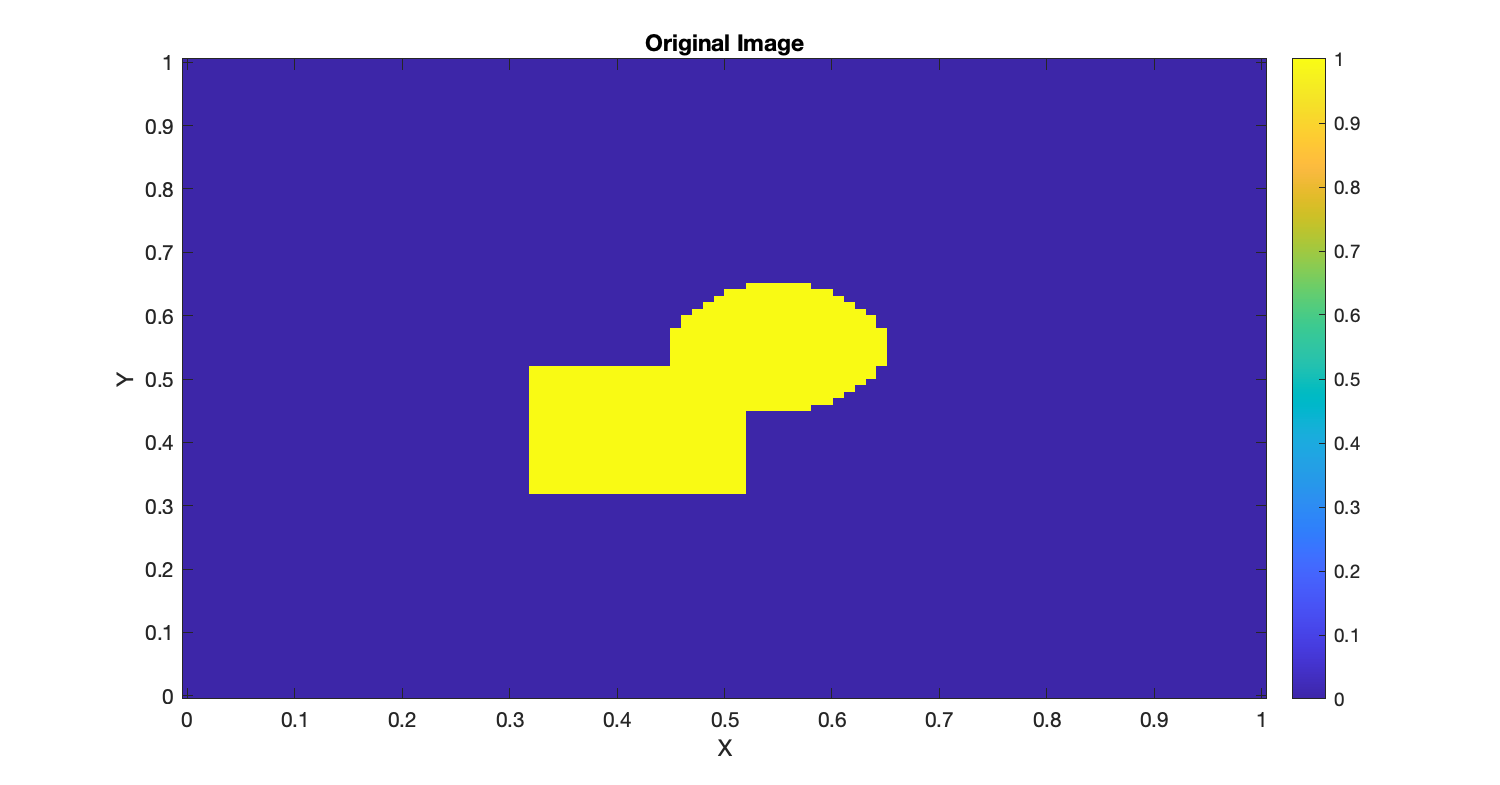
\includegraphics[width=0.5\textwidth]{original.png}}
  \hfill
  \subfloat[]{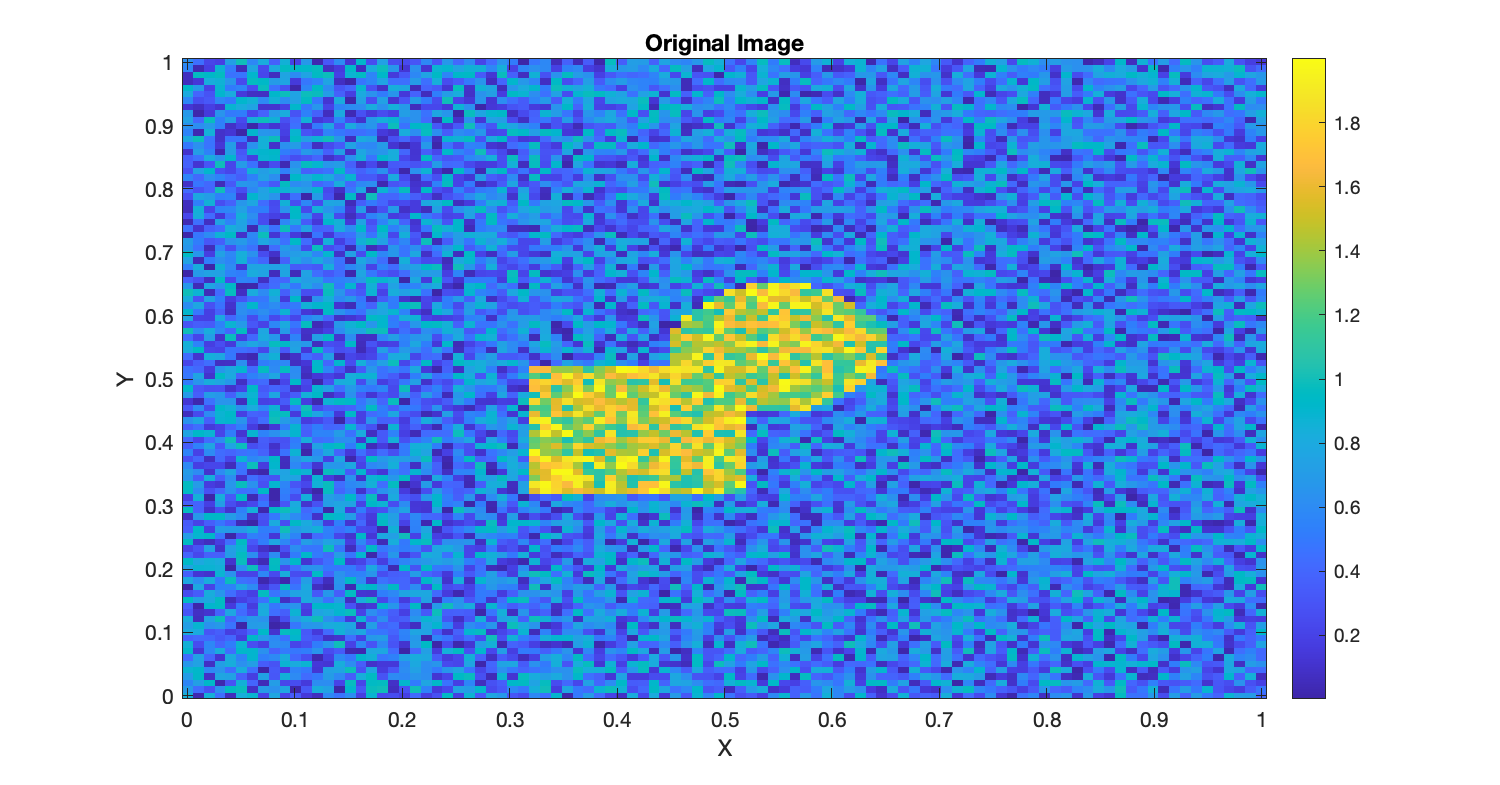
\includegraphics[width=0.5\textwidth]{noise.png}}
  \caption{(a) original image, (b)noisy image}
\end{figure}
Below are a series of images that show $|\nabla u_0|$ for increasing resolution, \underline{without} Gaussian smoother:
\begin{figure}[h!]
  \centering
  \subfloat[]{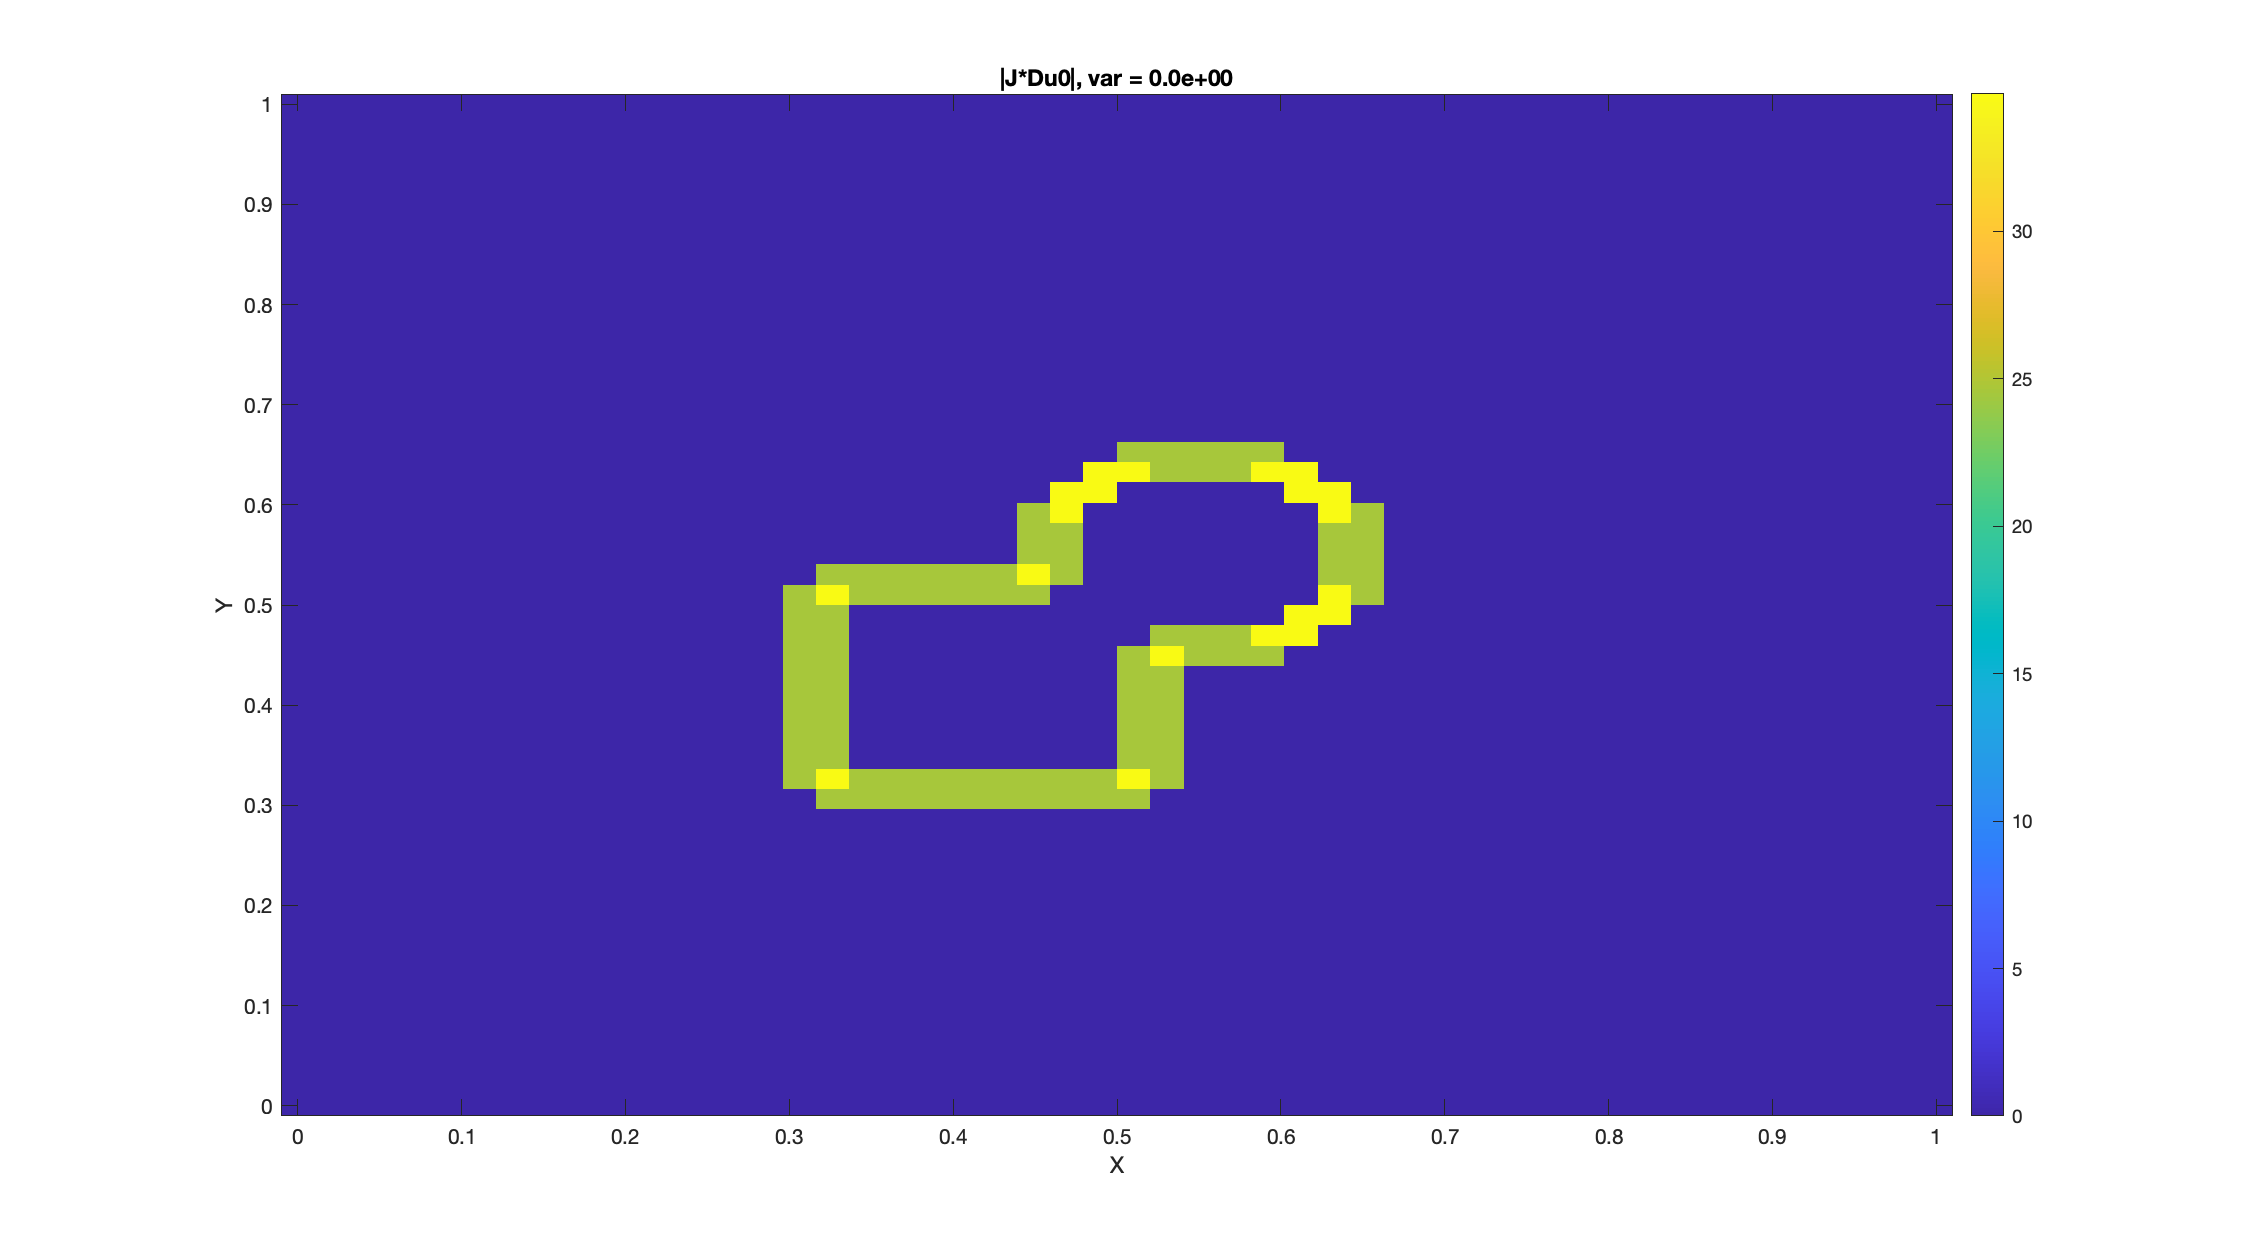
\includegraphics[width=0.5\textwidth]{d1.png}}
  \hfill
  \subfloat[]{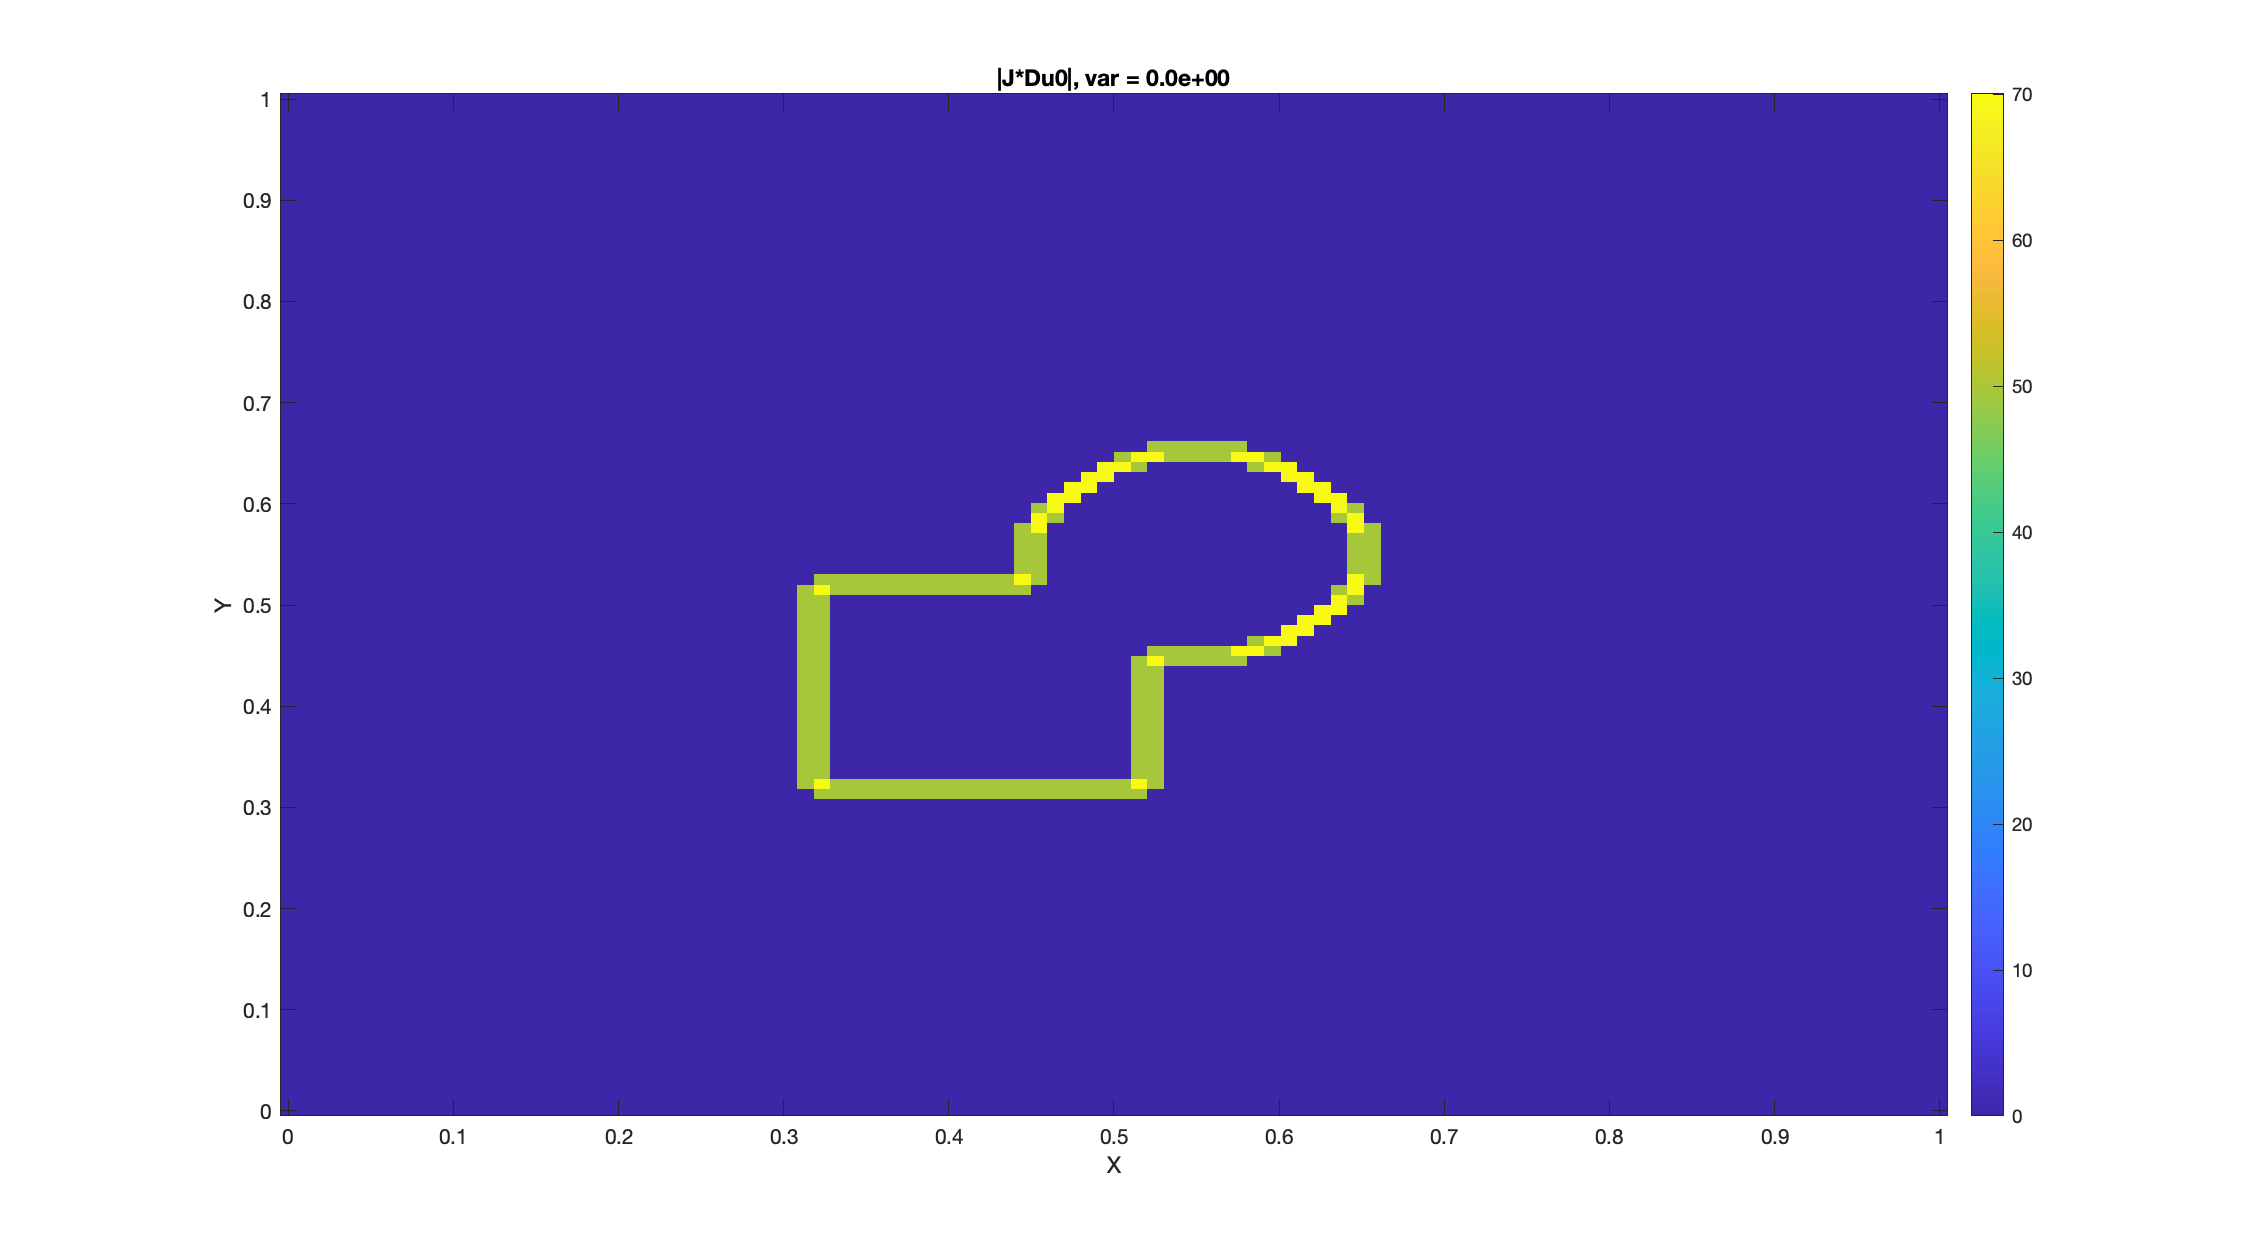
\includegraphics[width=0.5\textwidth]{d2.png}}\\
  \subfloat[]{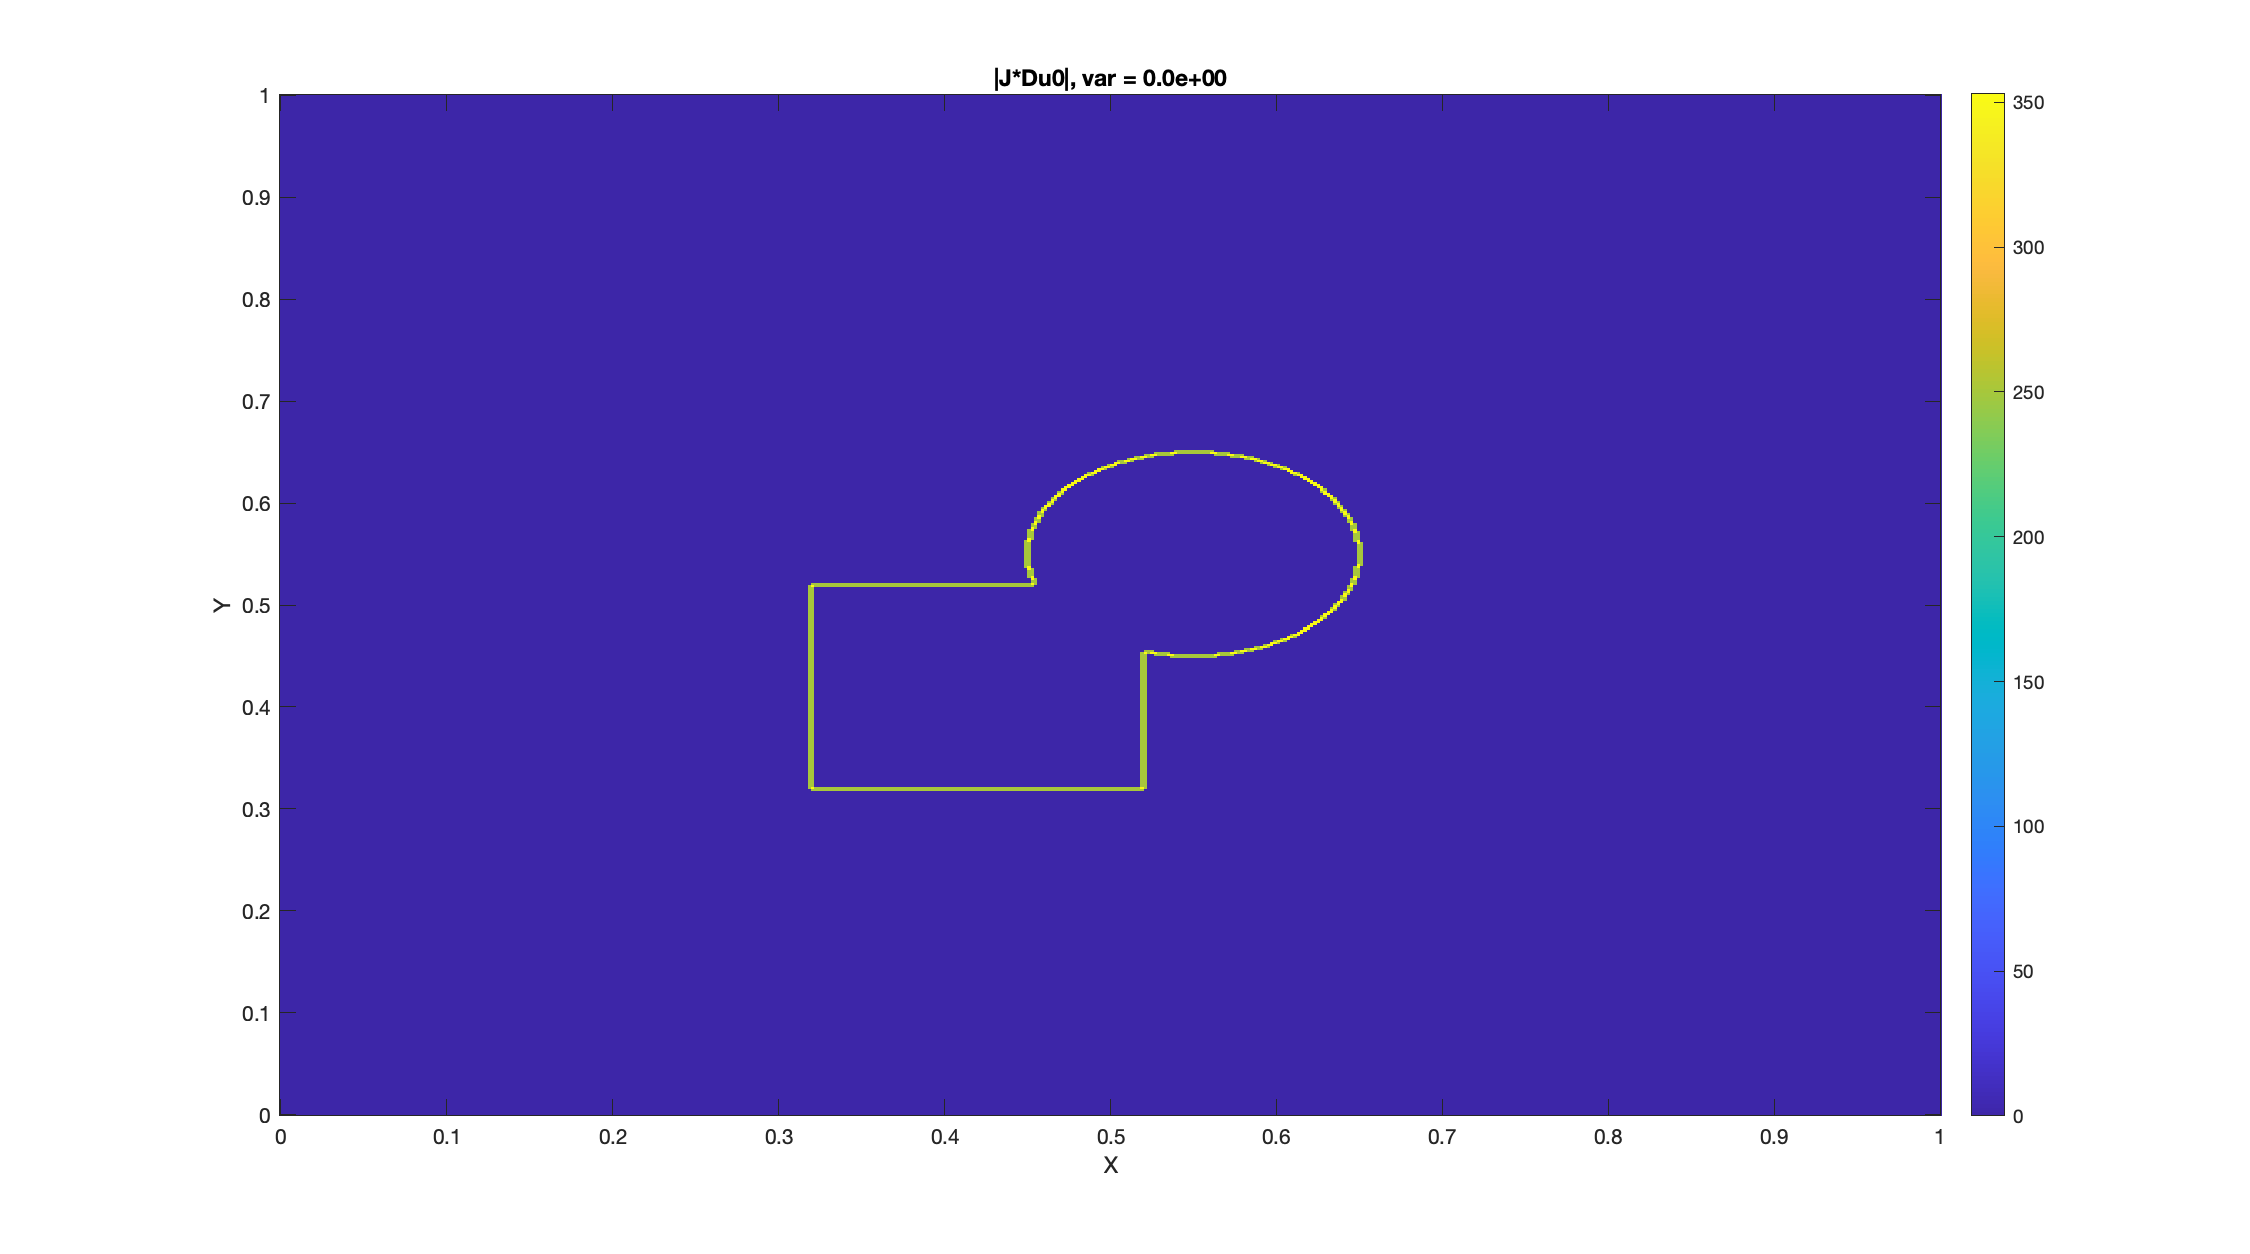
\includegraphics[width=0.5\textwidth]{d3.png}}
  \hfill
  \subfloat[]{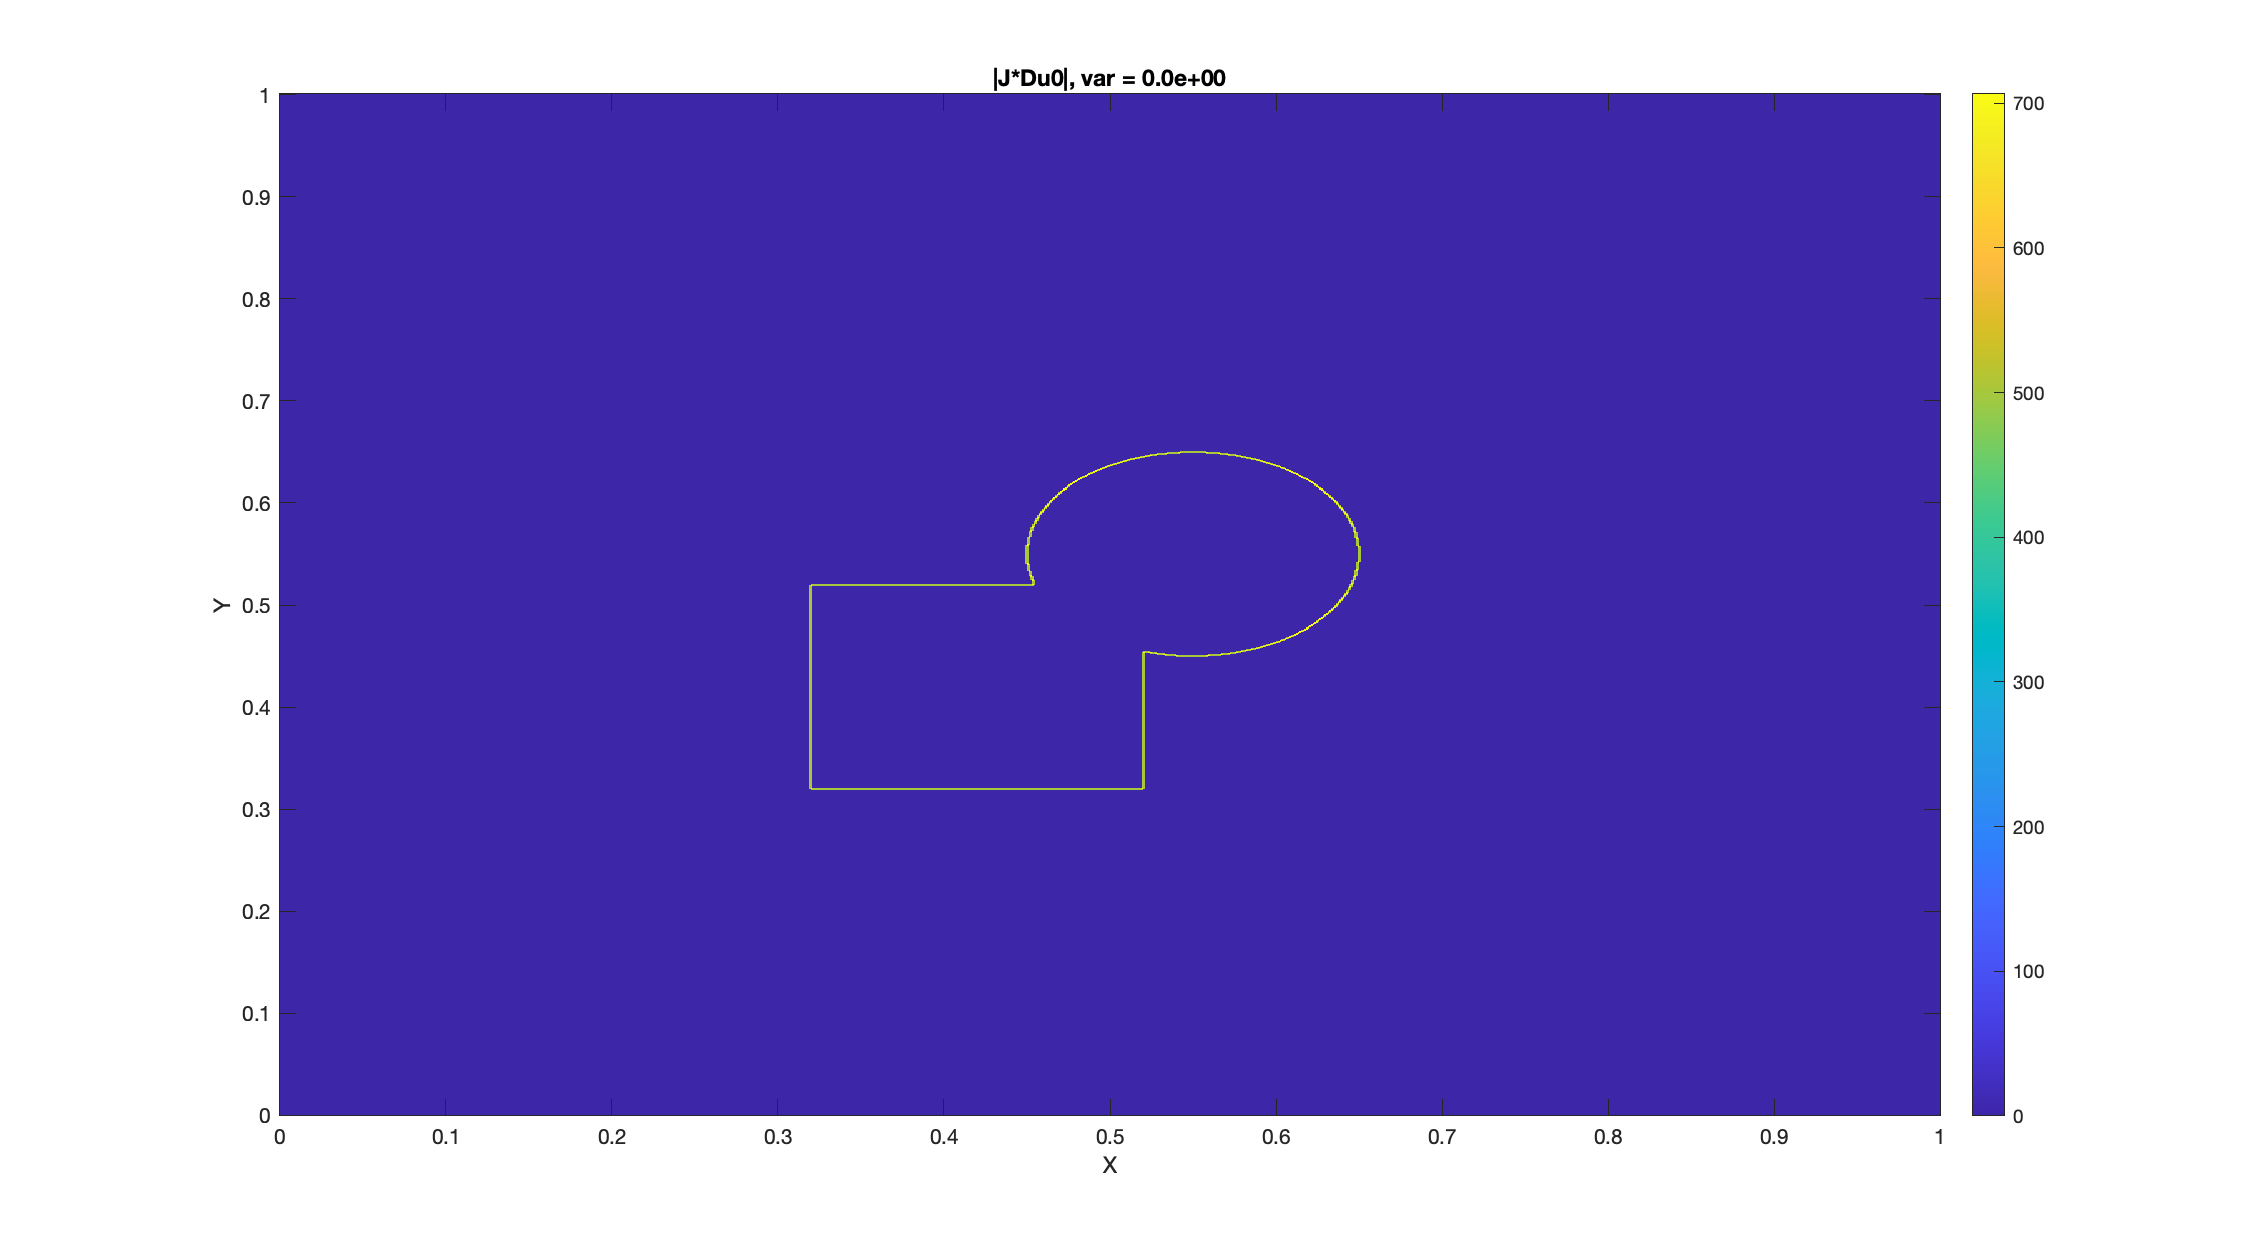
\includegraphics[width=0.5\textwidth]{d4.png}}
  \caption{Resolutions (a) 50x50, (b) 100x100, (c) 500x500, (d) 1000x1000}
\end{figure}

For increasing resolution our gradient in the image continues to grow; therefore, we need to smooth out the \textit{sharp} edges of the image. To do the smoothing with a given $\sigma$ I numerically solved the heat equation up to time $t=\sigma$, I utilized a Crank-Nicolson scheme in two dimensions analogous to LeVeque \cite{leveque2007finite} assuming $h_x=h_y=h$:
\[
\frac{U_{i,j}^{n+1}-U_{i,j}^n}{k}=\frac{1}{2}\left(\nabla^2U_{i,j}^n+\nabla^2U_{i,j}^{n+1}\right)
\]
where
\begin{align*}
    \nabla^2U_{i,j}^n&=\frac{U_{i-1,j}^n-2U_{i,j}^n+U_{i+1,j}^n}{h^2}+\frac{U_{i,j-1}^n-2U_{i,j}^n+U_{i,j+1}^n}{h^2}\\
    \nabla^2U_{i,j}^{n+1}&=\frac{U_{i-1,j}^{n+1}-2U_{i,j}^{n+1}+U_{i+1,j}^{n+1}}{h^2}+\frac{U_{i,j-1}^{n+1}-2U_{i,j}^{n+1}+U_{i,j+1}^{n+1}}{h^2}
\end{align*}
and I implemented Neumann boundary conditions $\partial U/\partial\eta=0$. Below is the implementation code:
\begin{lstlisting}
...
U = reshape(u,[],1); % initial conditions
% Matrix generation
K1D = spdiags(ones(nx,1)*[1 -2 1],-1:1,nx,nx)/h^2; % 1d Poisson matrix
I1D = speye(size(K1D)); % 1d identity matrix
K2D = kron(K1D,I1D)+kron(I1D,K1D); % 2d Poisson matrix
I2D = speye(size(K2D)); % 2d identity matrix
A = I2D-k/2*K2D; % LHS matrix for Crank-Nicolson
B = I2D+k/2*K2D; % RHS matrix for Crank-Nicolsons
ndpts = floor(3);
s = mit18086_stencil_stability((0:1:ndpts),1);
% Time loop
for j = 0:nt
    if j>0 % update step
        U = A\(B*U);
    end
    % for neumann b.c.
    U = weightedsum(U,s,nx);
end
U = reshape(U,nx,nx);
end
\end{lstlisting}
\clearpage
Below are images of the smoothed out noisey image for different variance $\sigma$:
\begin{figure}[h!]
  \centering
  \subfloat[]{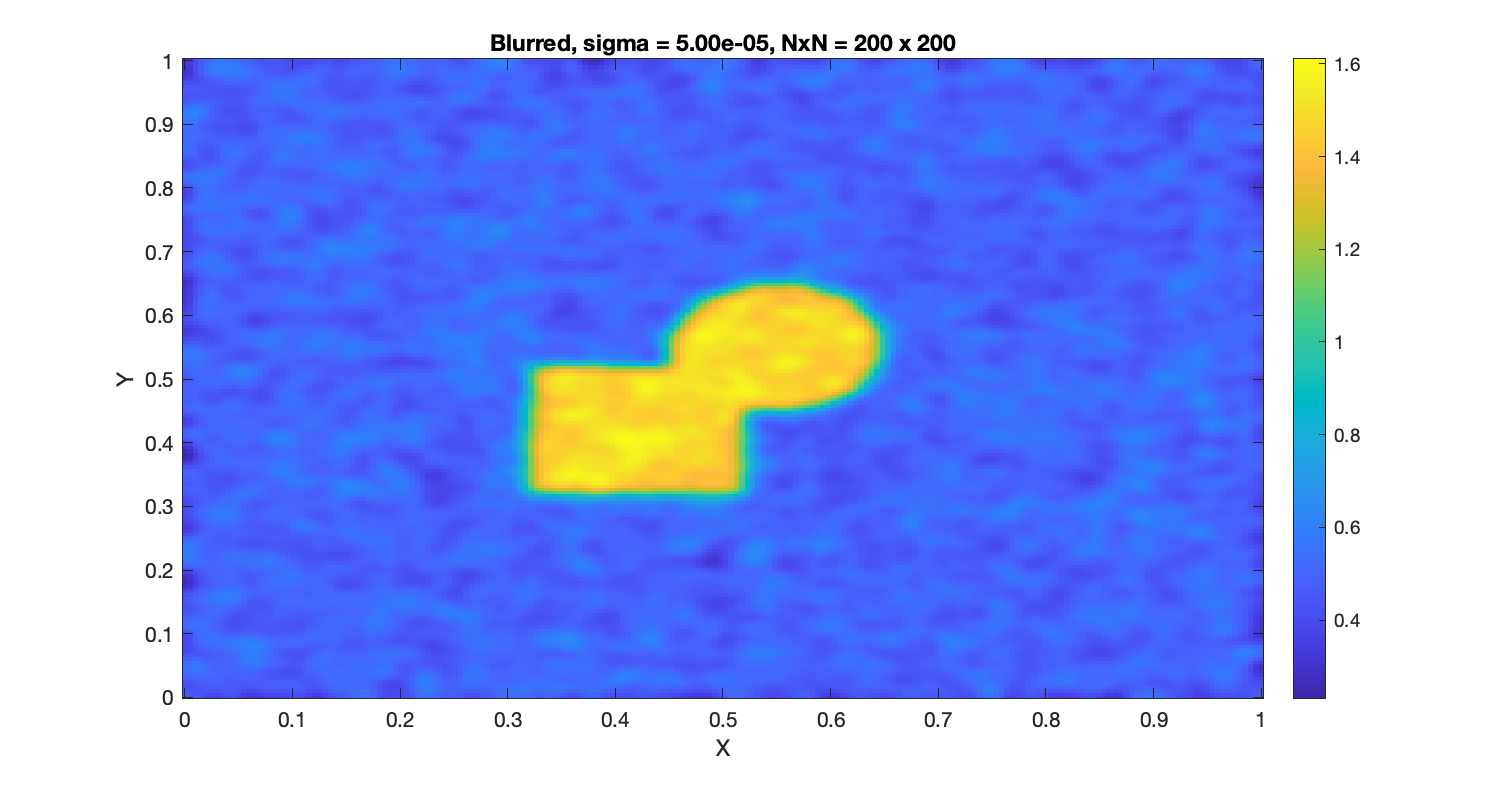
\includegraphics[width=0.5\textwidth]{n1.png}}
  \hfill
  \subfloat[]{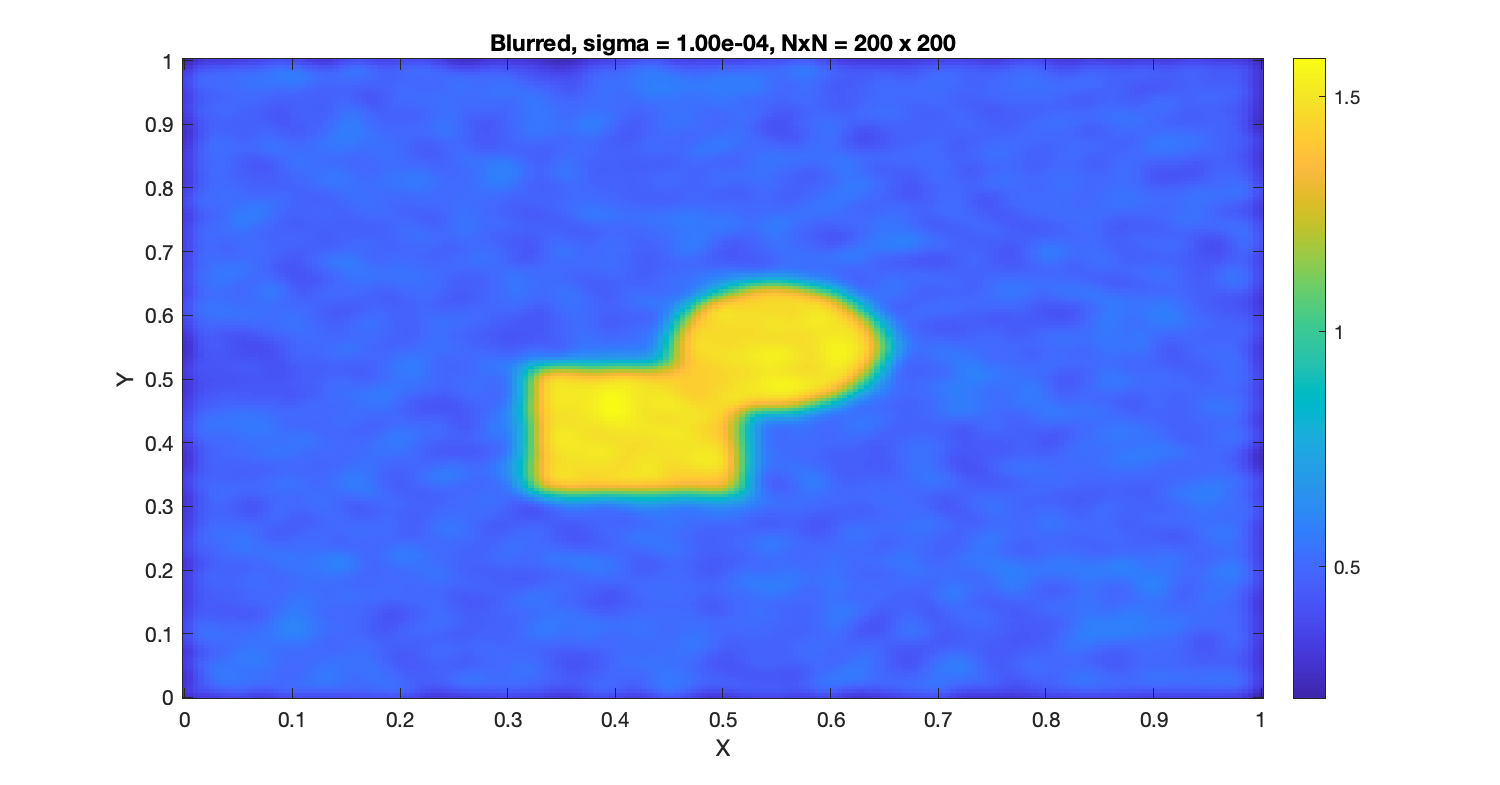
\includegraphics[width=0.5\textwidth]{n2.png}}\\
  \subfloat[]{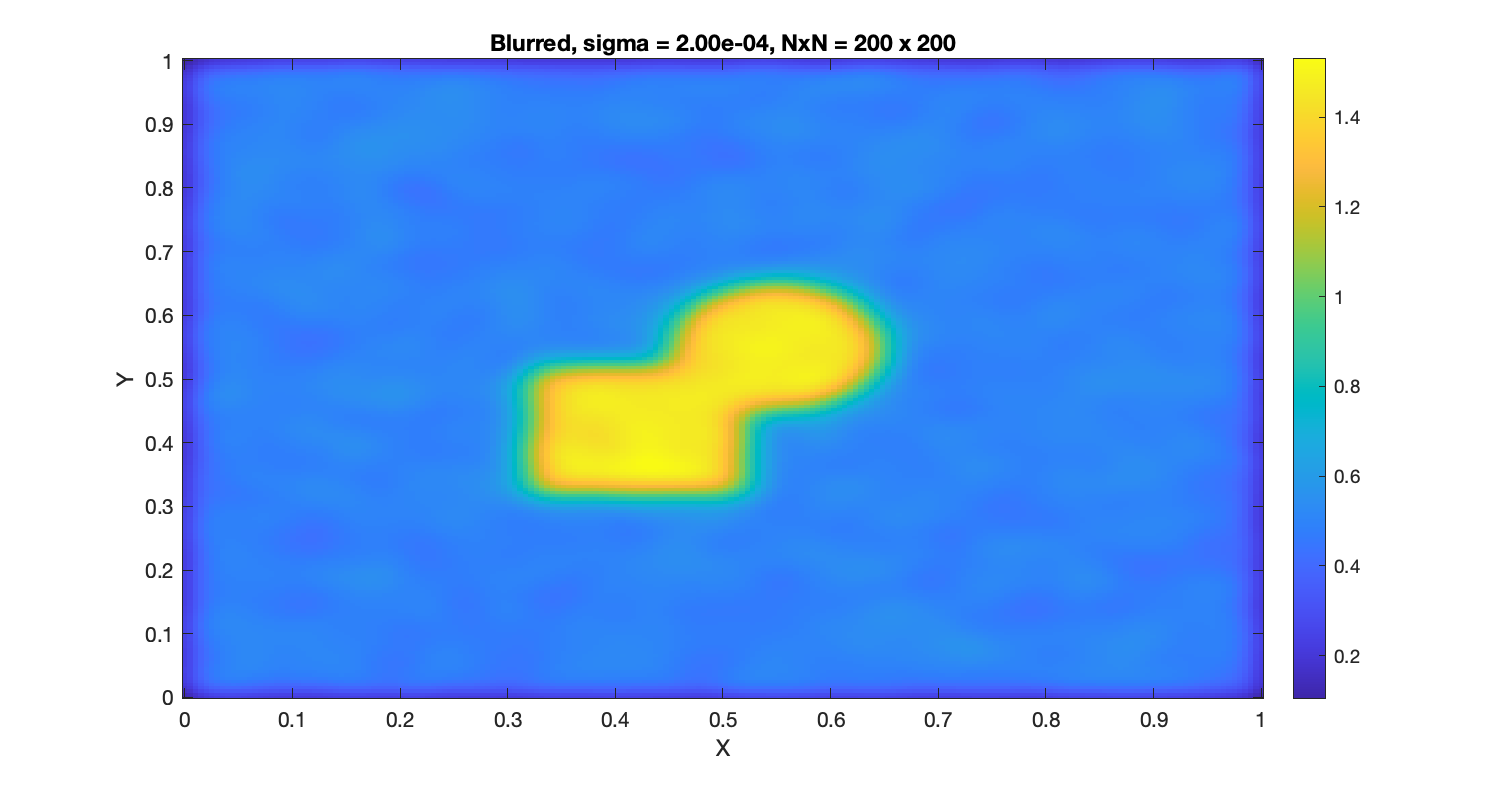
\includegraphics[width=0.5\textwidth]{n3.png}}
  \hfill
  \subfloat[]{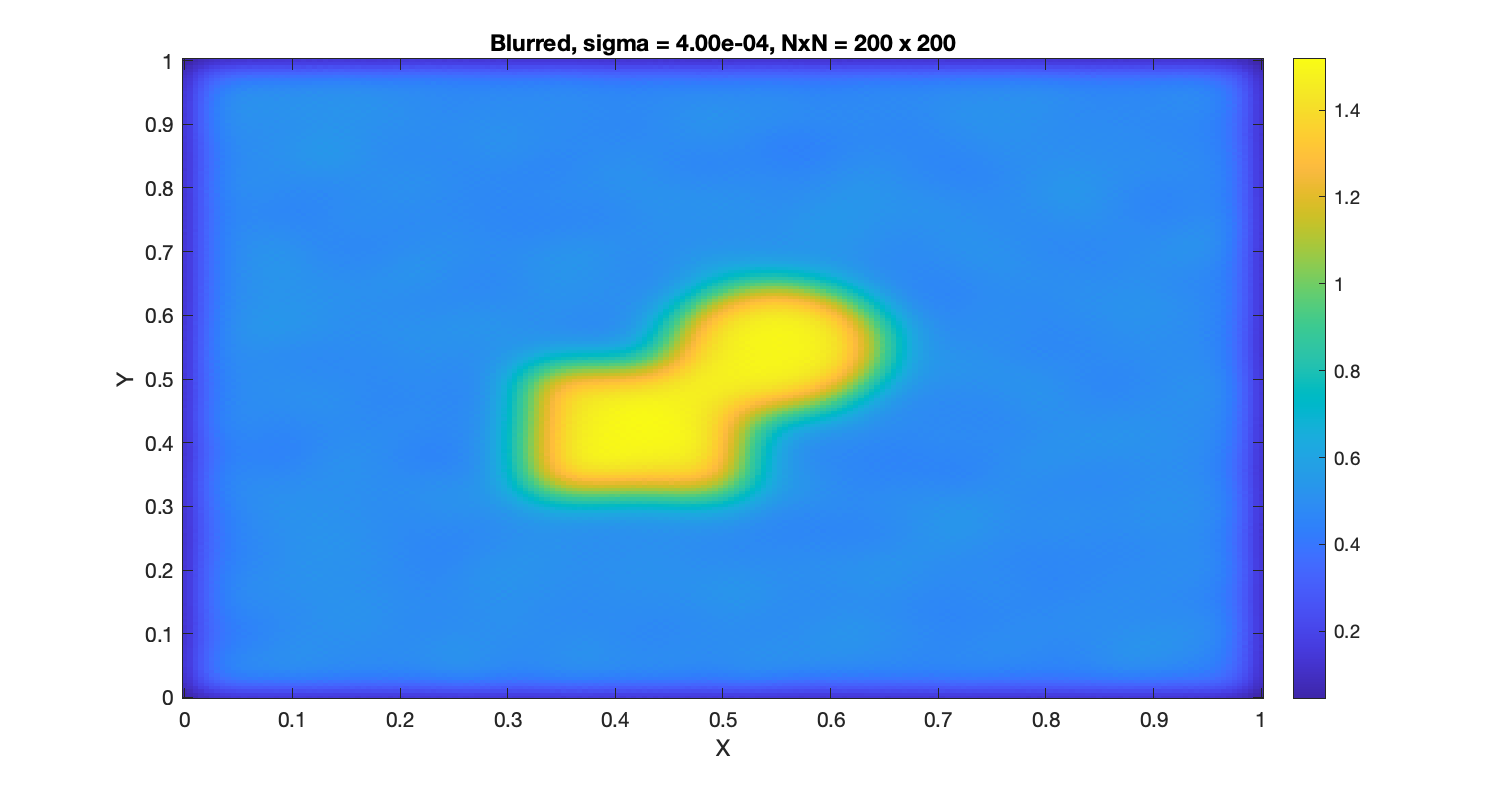
\includegraphics[width=0.5\textwidth]{n4.png}}
  \caption{Variance (a) $5\times 10^{-5}$, (b) $1\times 10^{-4}$, (c) $2\times 10^{-4}$, (d) $4\times 10^{-4}$}
\end{figure}

Another important point to address is how the variance $\sigma$ and the width of the smoothing are related. To do this we can analytically solve the heat equation with Dirac initial data:
\[
\begin{cases}
u_t = -\nabla^2u & \vec{x}\in\Omega, t>0\\
u(x,0)= \delta_0(x)
\end{cases}
\]
the solution to this is the fundamental solution \cite{evans2010partial}:
\[
\Phi(\vec{x},t)=\frac{1}{4\pi t}e^{-|\vec{x}|^2/(4t)}
\]
the amount of smoothing is determined by $t=\sigma>0$; therefore,
\[
\Phi(\vec{x},\sigma)=\frac{1}{4\pi \sigma}e^{-|\vec{x}|^2/(4\sigma)}
\]
The maximum occurs when $\vec{x}=0$; therefore, $\Phi_{max}=1/(4\pi \sigma)$. Now the width of the smoothing can be given by when $\Phi$ is $5\%$ of the maximum; therefore, we need to solve
\[
0.05\cdot\frac{1}{4\pi\sigma}=\frac{1}{4\pi \sigma}e^{-d^2/(4\sigma)}
\]
which has solution given by
\[
d = 2\sqrt{\sigma\ln(20)}.
\]
\clearpage
As an example consider:
\begin{figure}[h!]
    \centering
    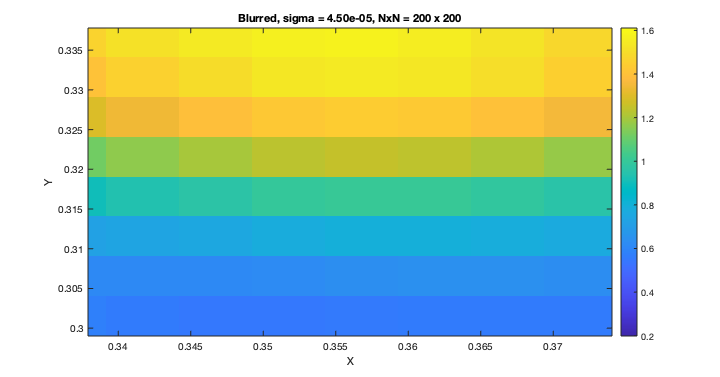
\includegraphics[width = 0.6\linewidth]{blurrEX.png}
    \caption{$\sigma=4.5\times 10^{-5}$}
\end{figure}

Here the variance $\sigma = 4.5\times 10^{-5}$ can be plugged in to our relationship to get $d = 0.0232$ which is about the width of the smoothing region. Also we have that the grid resolution is $h=1/200<d$, therefore we capture the smoothing regions of our image. However if we have resolution more than the smoothing width we lose the smoothing region:
\begin{figure}[h!]
    \centering
    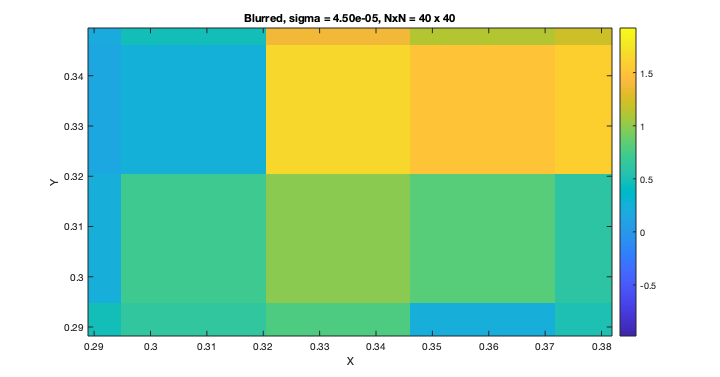
\includegraphics[width = 0.6\linewidth]{blurrEX2.png}
    \caption{$\sigma=4.5\times 10^{-5}$ and $h=1/40$}
\end{figure}

this will cause the level set front to encounter very high jumps, that is large gradients. Now we have a relationship between $\sigma$ and $d$ the smoothing width, this will allows us to carefully choose $p$ and $\gamma$. We want $p$ and $\gamma$ to be such that $|\nabla g(\nabla u_0)|$ is order magnitude of $1/d$.
\section{Numerical Method} To establish the numerical scheme, I will write out the terms for the \textit{generalized curvature} given in our PDE equation
\[
\underbrace{A\nabla\cdot\frac{\nabla\phi}{|\nabla\phi|}}_{\textrm{Part 1}}+\underbrace{\nabla A\cdot\frac{\nabla\phi}{|\nabla\phi|}}_{\textrm{Part 2}}
\]
where $A = g(\nabla u_0)$, I will do this in two parts. For Part 1 we have, Part 1
\begin{align*}
    &=A(\partial_x,\partial_y)\cdot\frac{(\phi_x,\phi_y)}{(\phi_x^2+\phi_y^2)^{1/2}}\\[4pt]
    &=A\left(\partial_x\left(\frac{\phi_x}{(\phi_x^2+\phi_y^2)^{1/2}}\right)+\partial_y\left(\frac{\phi_y}{(\phi_x^2+\phi_y^2)^{1/2}}\right)\right)\\
    &=A\left(\frac{|\nabla\phi|\phi_{xx}-\phi_x\frac{1}{|\nabla\phi|}(\phi_x\phi_{xx}+\phi_y\phi_{yx})}{|\nabla\phi|^2}+\frac{|\nabla\phi|\phi_{yy}-\phi_y\frac{1}{|\nabla\phi|}(\phi_x\phi_{xy}+\phi_y\phi_{yy})}{|\nabla\phi|^2}\right)\\
    &=\frac{A}{|\nabla\phi|^3}\left(|\nabla\phi|^2\phi_{xx}-\phi_x^2\phi_{xx}-2\phi_x\phi_y\phi_{xy}-\phi_y^2\phi_{yy}+|\nabla\phi|^2\phi_{yy}\right)
\end{align*}
which is coded as
\begin{lstlisting}
F1=(A.*((Pxx.*Py.^2-Px.*Py.*Pxy)+...
   (Pyy.*Px.^2-Px.*Py.*Pxy)))./((Px.^2+Py.^2).^(1.5));
\end{lstlisting}
For the Part 2, I do an entry wise finite difference to compute $A_x$ and $A_y$
\begin{lstlisting}
Ax = (A(3:end,:)-A(1:end-2,:))/(2*h); 
Ax = Ax([1 1:end end],:);
Ay = (A(:,3:end)-A(:,1:end-2))/(2*h); 
Ay = Ay(:,[1 1:end end]);
\end{lstlisting}
then I add both terms
\begin{lstlisting}
F2=(Ax.*Px+Ay.*Py)./((Px.^2+Py.^2).^(0.5));
F=(F1+F2);
F = min(max(F,-spd/h),spd/h);
\end{lstlisting}
note that I have a parameter ``spd'' to control the speed of the front, as it is possible for the level set to develop sharp cut-ins, this means that the front is moving too fast in some locations. The remaining multiplication of $|\nabla\phi|$ is treated as
\[
|\nabla\phi|=(\phi_x^2+\phi_y^2)^{1/2}
\]
and is multiplied by the generalized curvature which I call ``F'' and the code is below:
\begin{lstlisting}
DxP = diff(P)/h;   DxmP = DxP([1 1:end],:); DxpP = DxP([1:end end],:);
DyP = diff(P')'/h; DymP = DyP(:,[1 1:end]); DypP = DyP(:,[1:end end]);
Np = sqrt(max(DxmP,0).^2+min(DxpP,0).^2+max(DymP,0).^2+min(DypP,0).^2);
Nm = sqrt(min(DxmP,0).^2+max(DxpP,0).^2+min(DymP,0).^2+max(DypP,0).^2);
dP = max(F,0).*(Np-c)+min(F,0).*(Nm-c);
\end{lstlisting}
Then I use a FE update rule taking into account the signage of the curvature term:
\begin{lstlisting}
for it = 1:nt 
   F = -curvature(A,P,h,spd)*5e-3;     % movement under curvature
   P = P-dt*FabsgradP(P,h,F);      % level set update
end
\end{lstlisting}
For the edge detector (\ref{eqn2}) I have two input parameters which will contribute to the movement of the level set front, the two parameters are given by $\gamma$ and $p$. In the next section I demonstrate the results for different values of $\gamma$ and $p$ and also for different variance $\sigma$. 
\clearpage
\section{Results}
For this section I demonstrate the results for different parameters of $p$, $\gamma$, and $\sigma$. Below is an example that demonstrates the original image and the resolved image
\begin{figure}[h!]
  \centering
  \subfloat[]{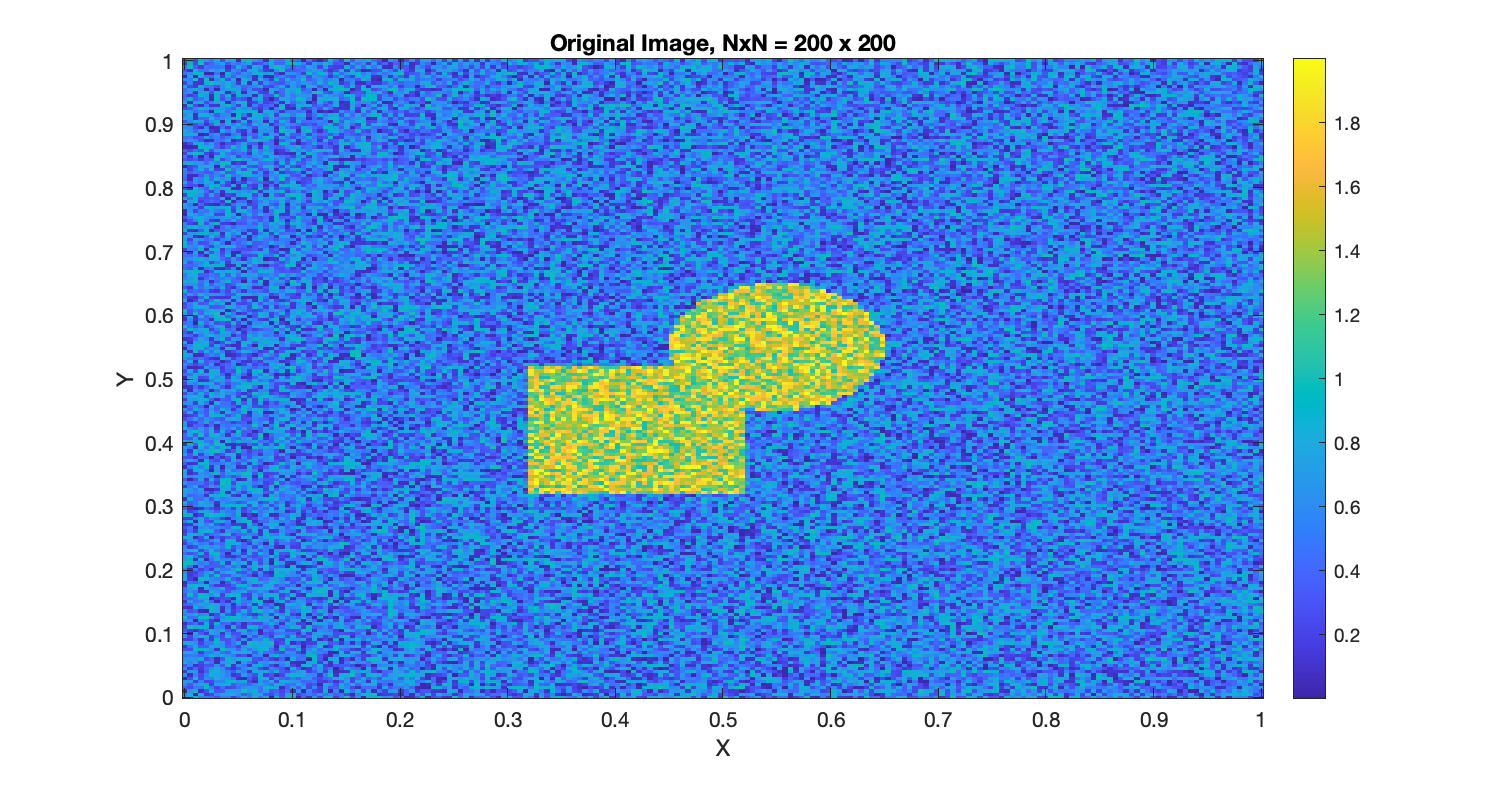
\includegraphics[width=0.5\textwidth]{ex1.png}}
  \hfill
  \subfloat[]{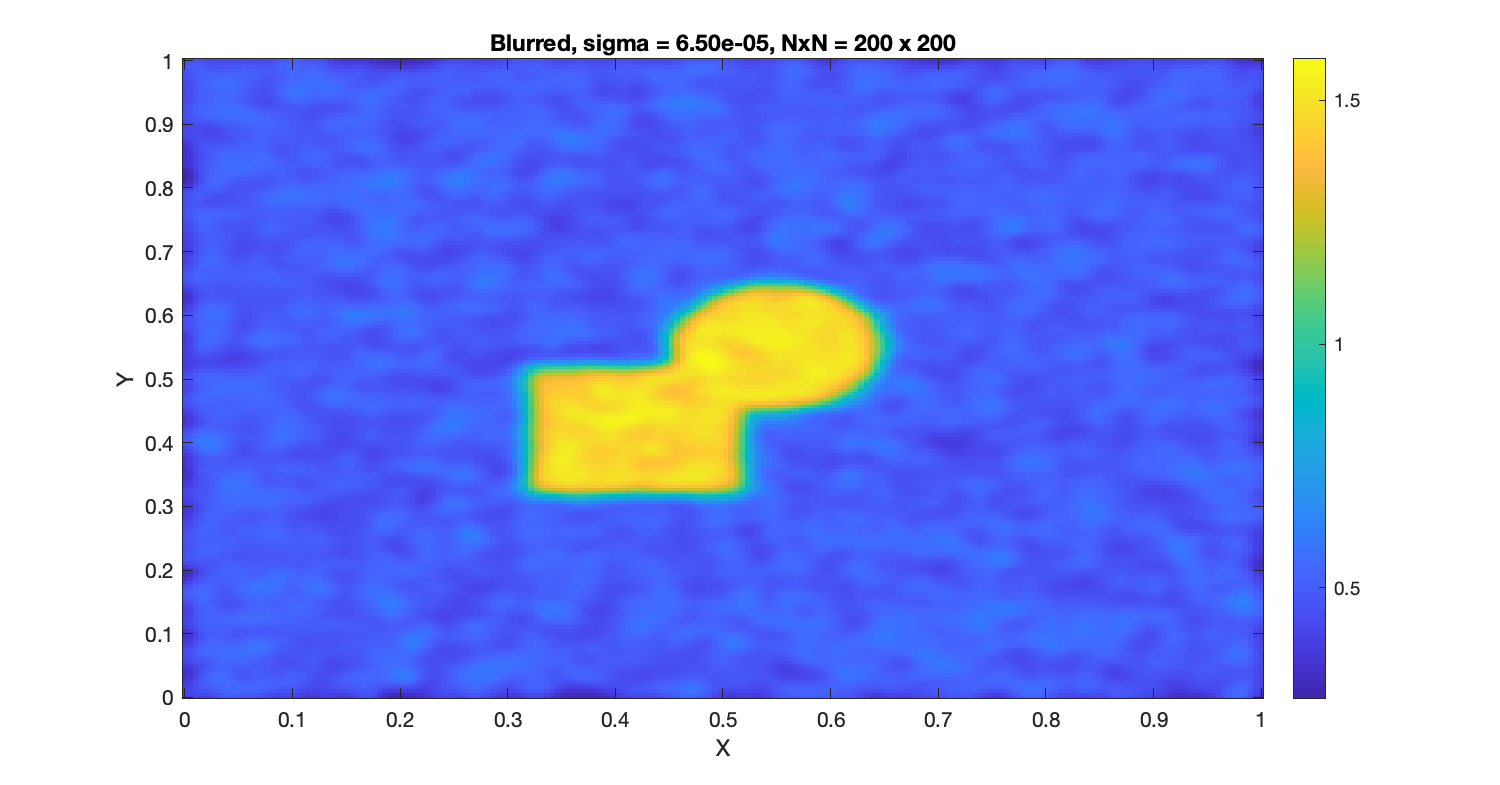
\includegraphics[width=0.5\textwidth]{ex1blurred.png}}\\
  \subfloat[]{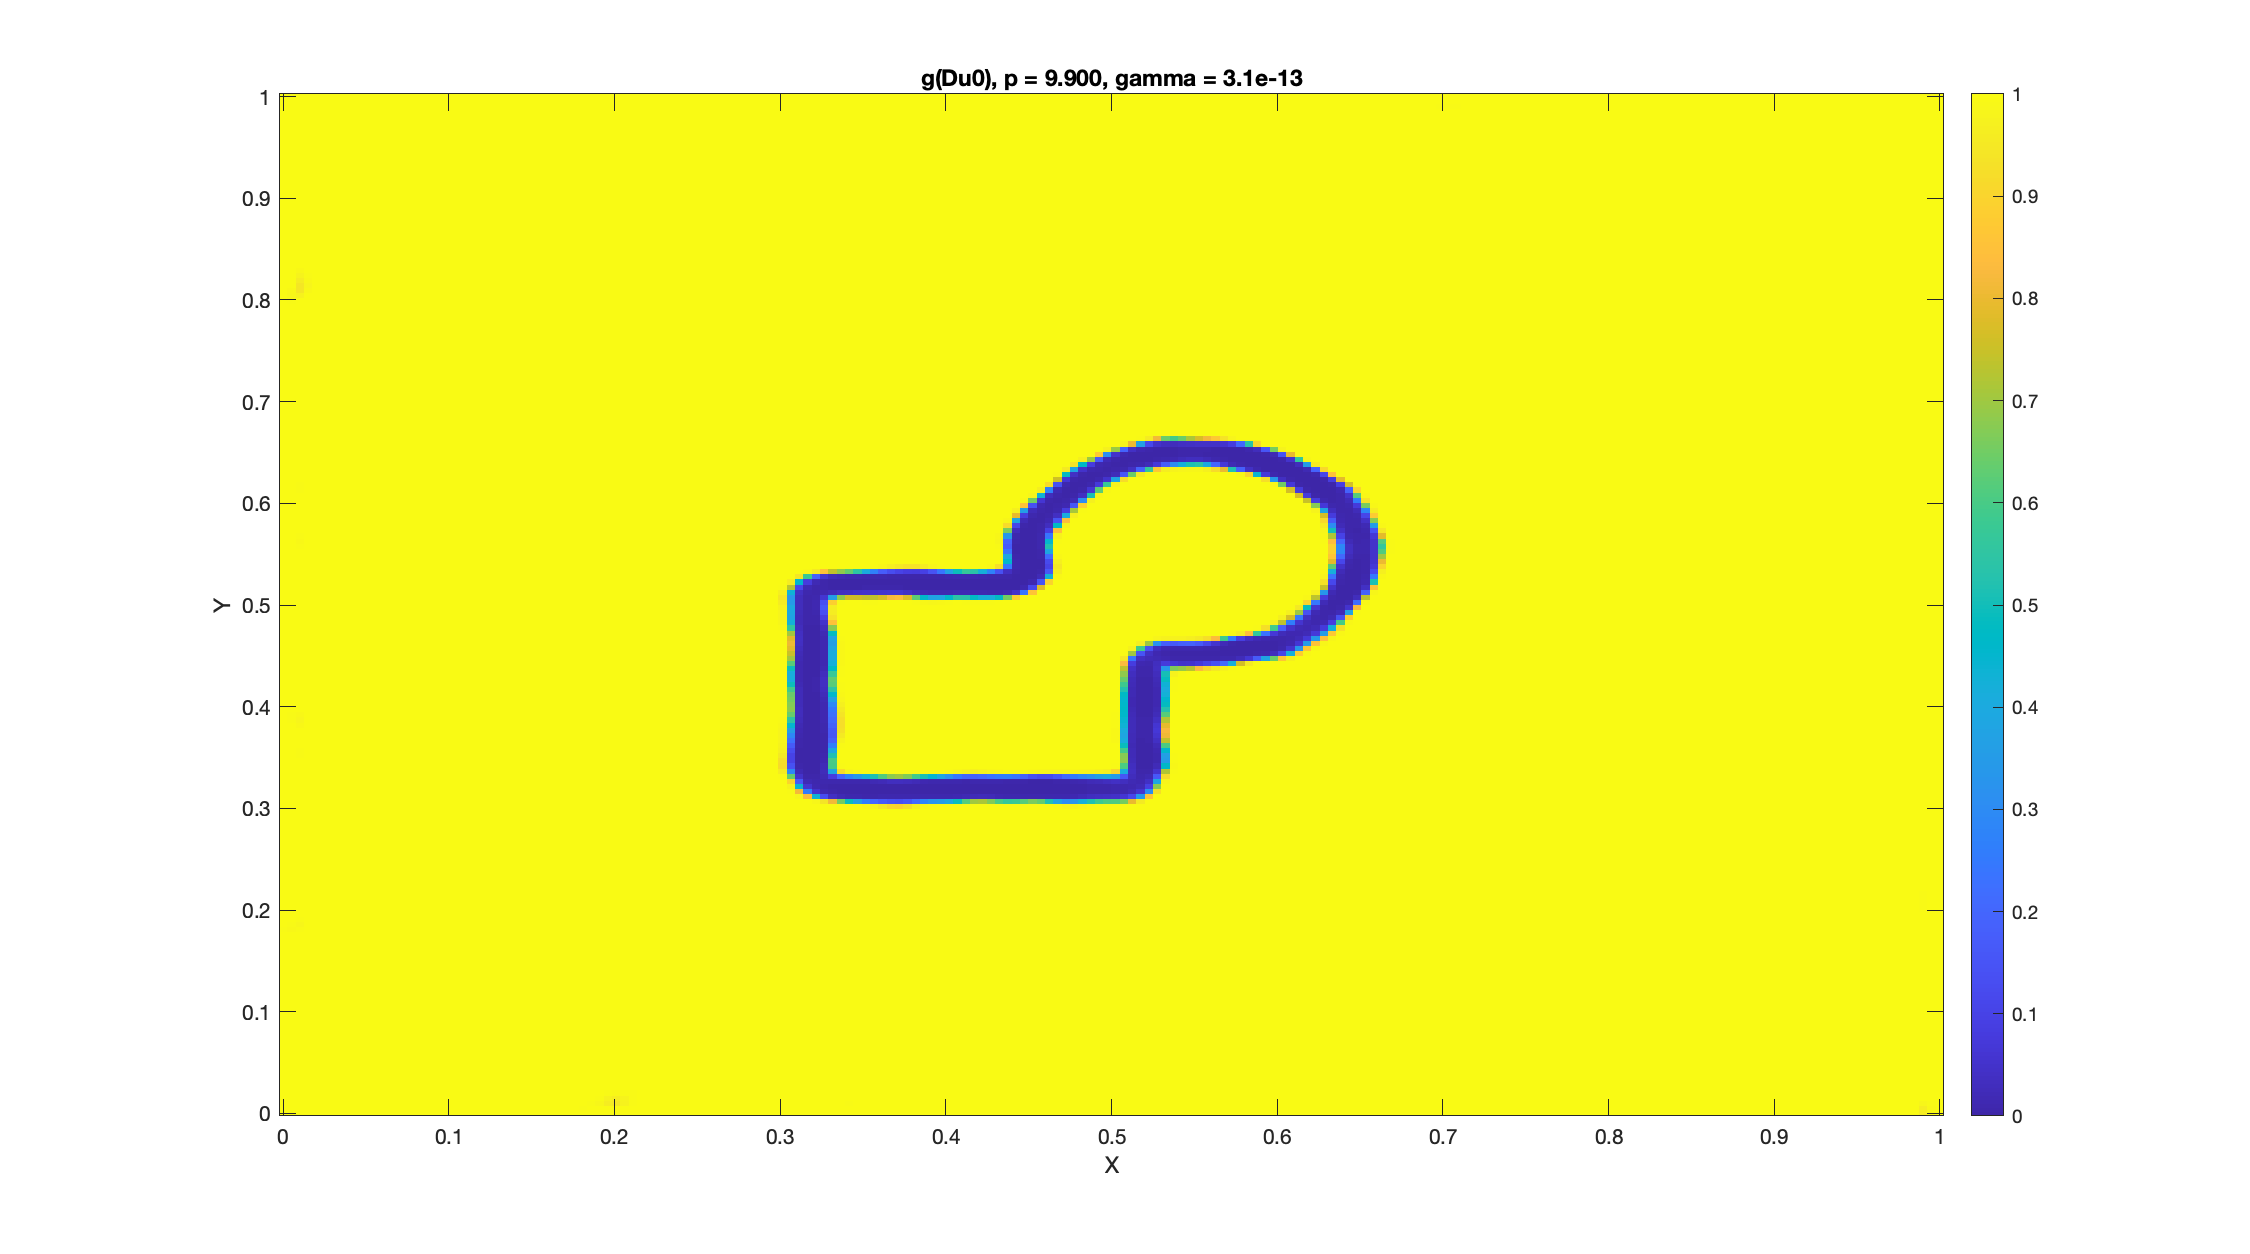
\includegraphics[width=0.5\textwidth]{ex1spd.png}}
  \\
  \subfloat[]{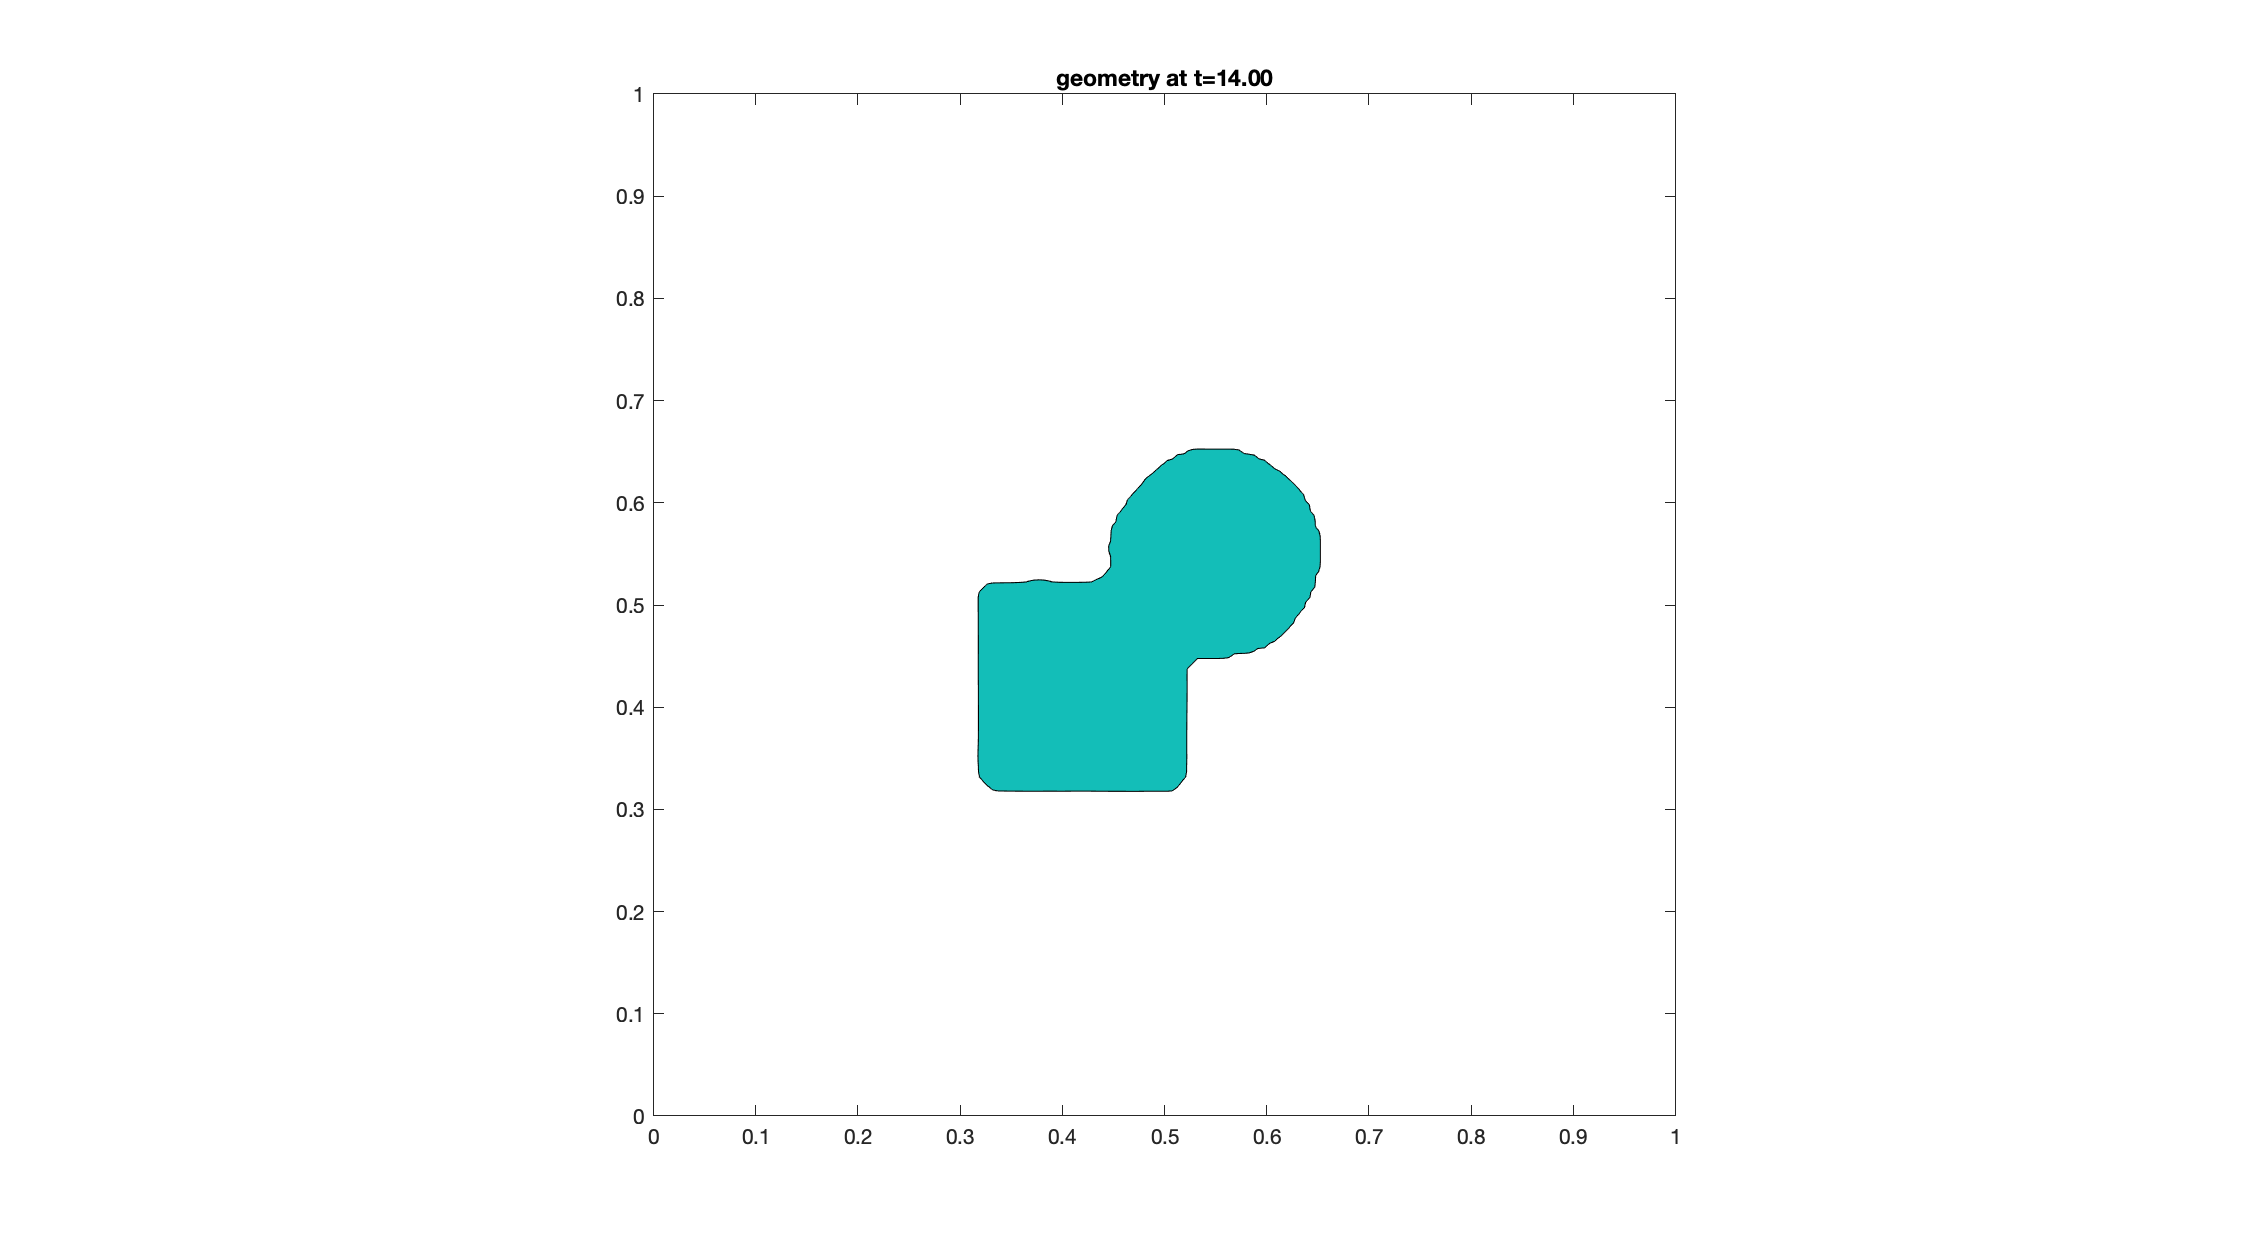
\includegraphics[width=0.5\textwidth]{ex1final.png}}
  \caption{$\sigma = 6.5\times 10^{-5}$, $p = 9.9$, $\gamma=5.5\times 10^{-13.25}$}
\end{figure}
If I divide $p$ in half I get
\clearpage
\begin{figure}[h!]
  \centering
  \subfloat[]{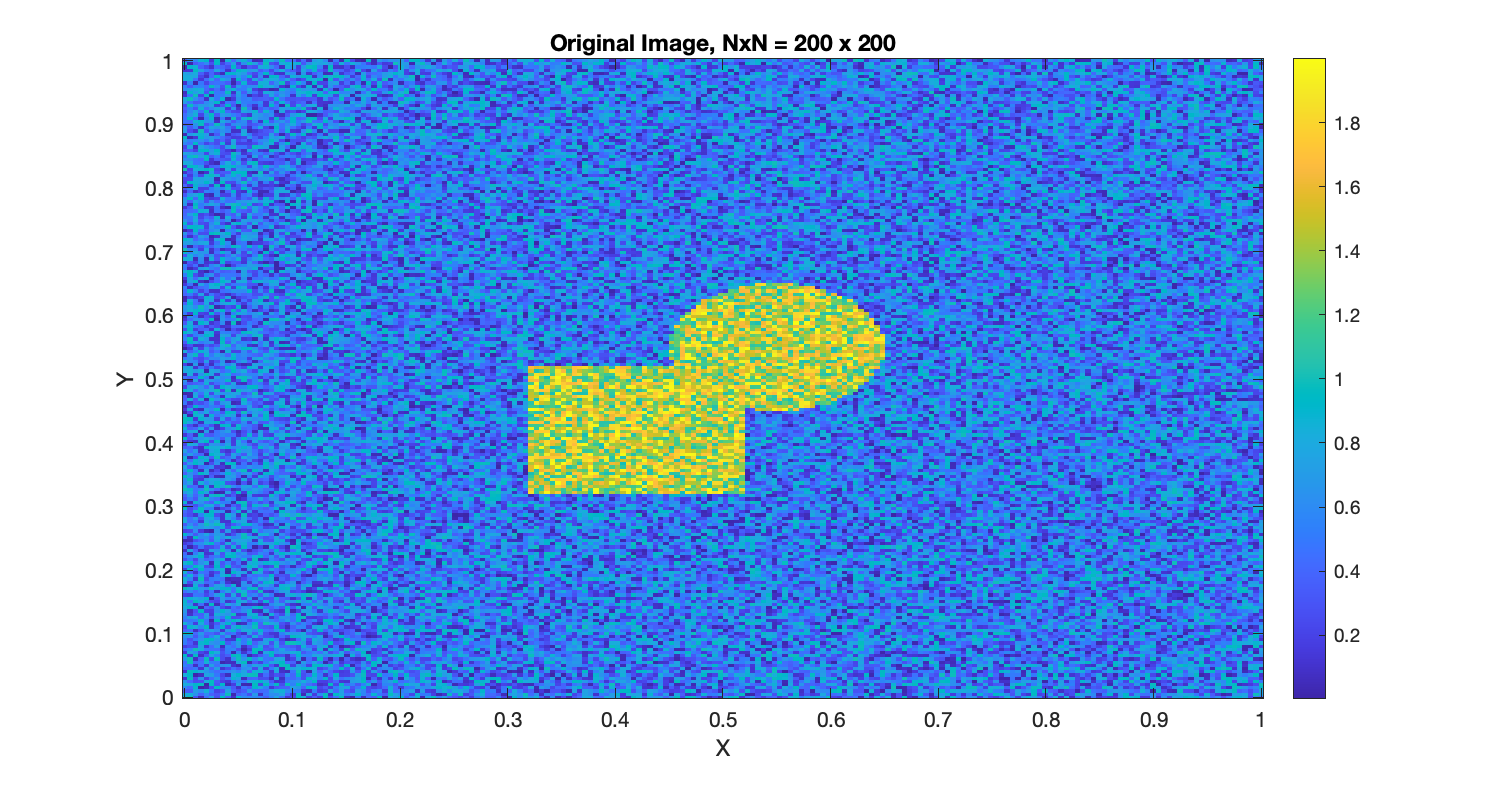
\includegraphics[width=0.5\textwidth]{ex2original.png}}
  \hfill
  \subfloat[]{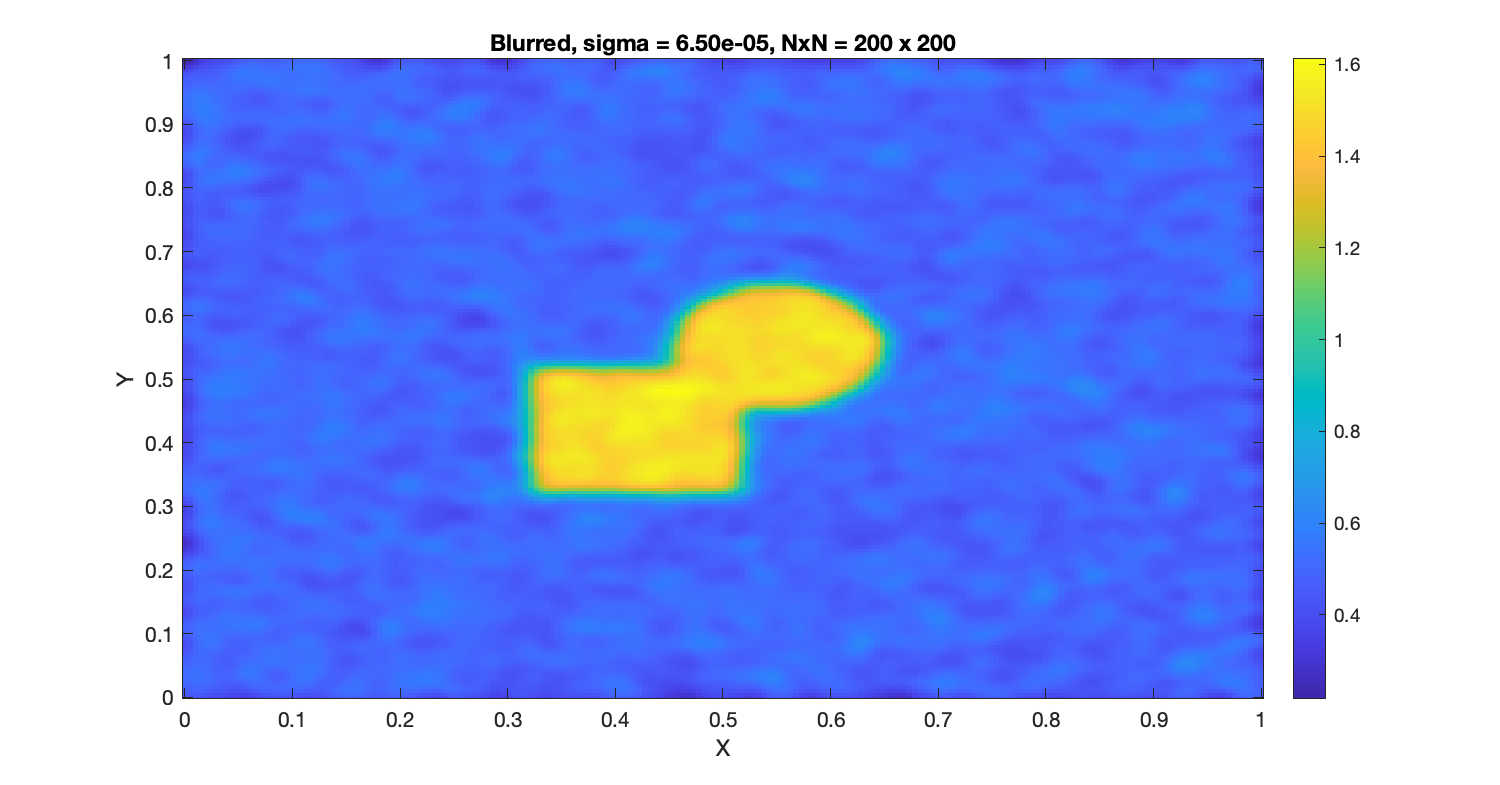
\includegraphics[width=0.5\textwidth]{ex2blurred.png}}\\
  \subfloat[]{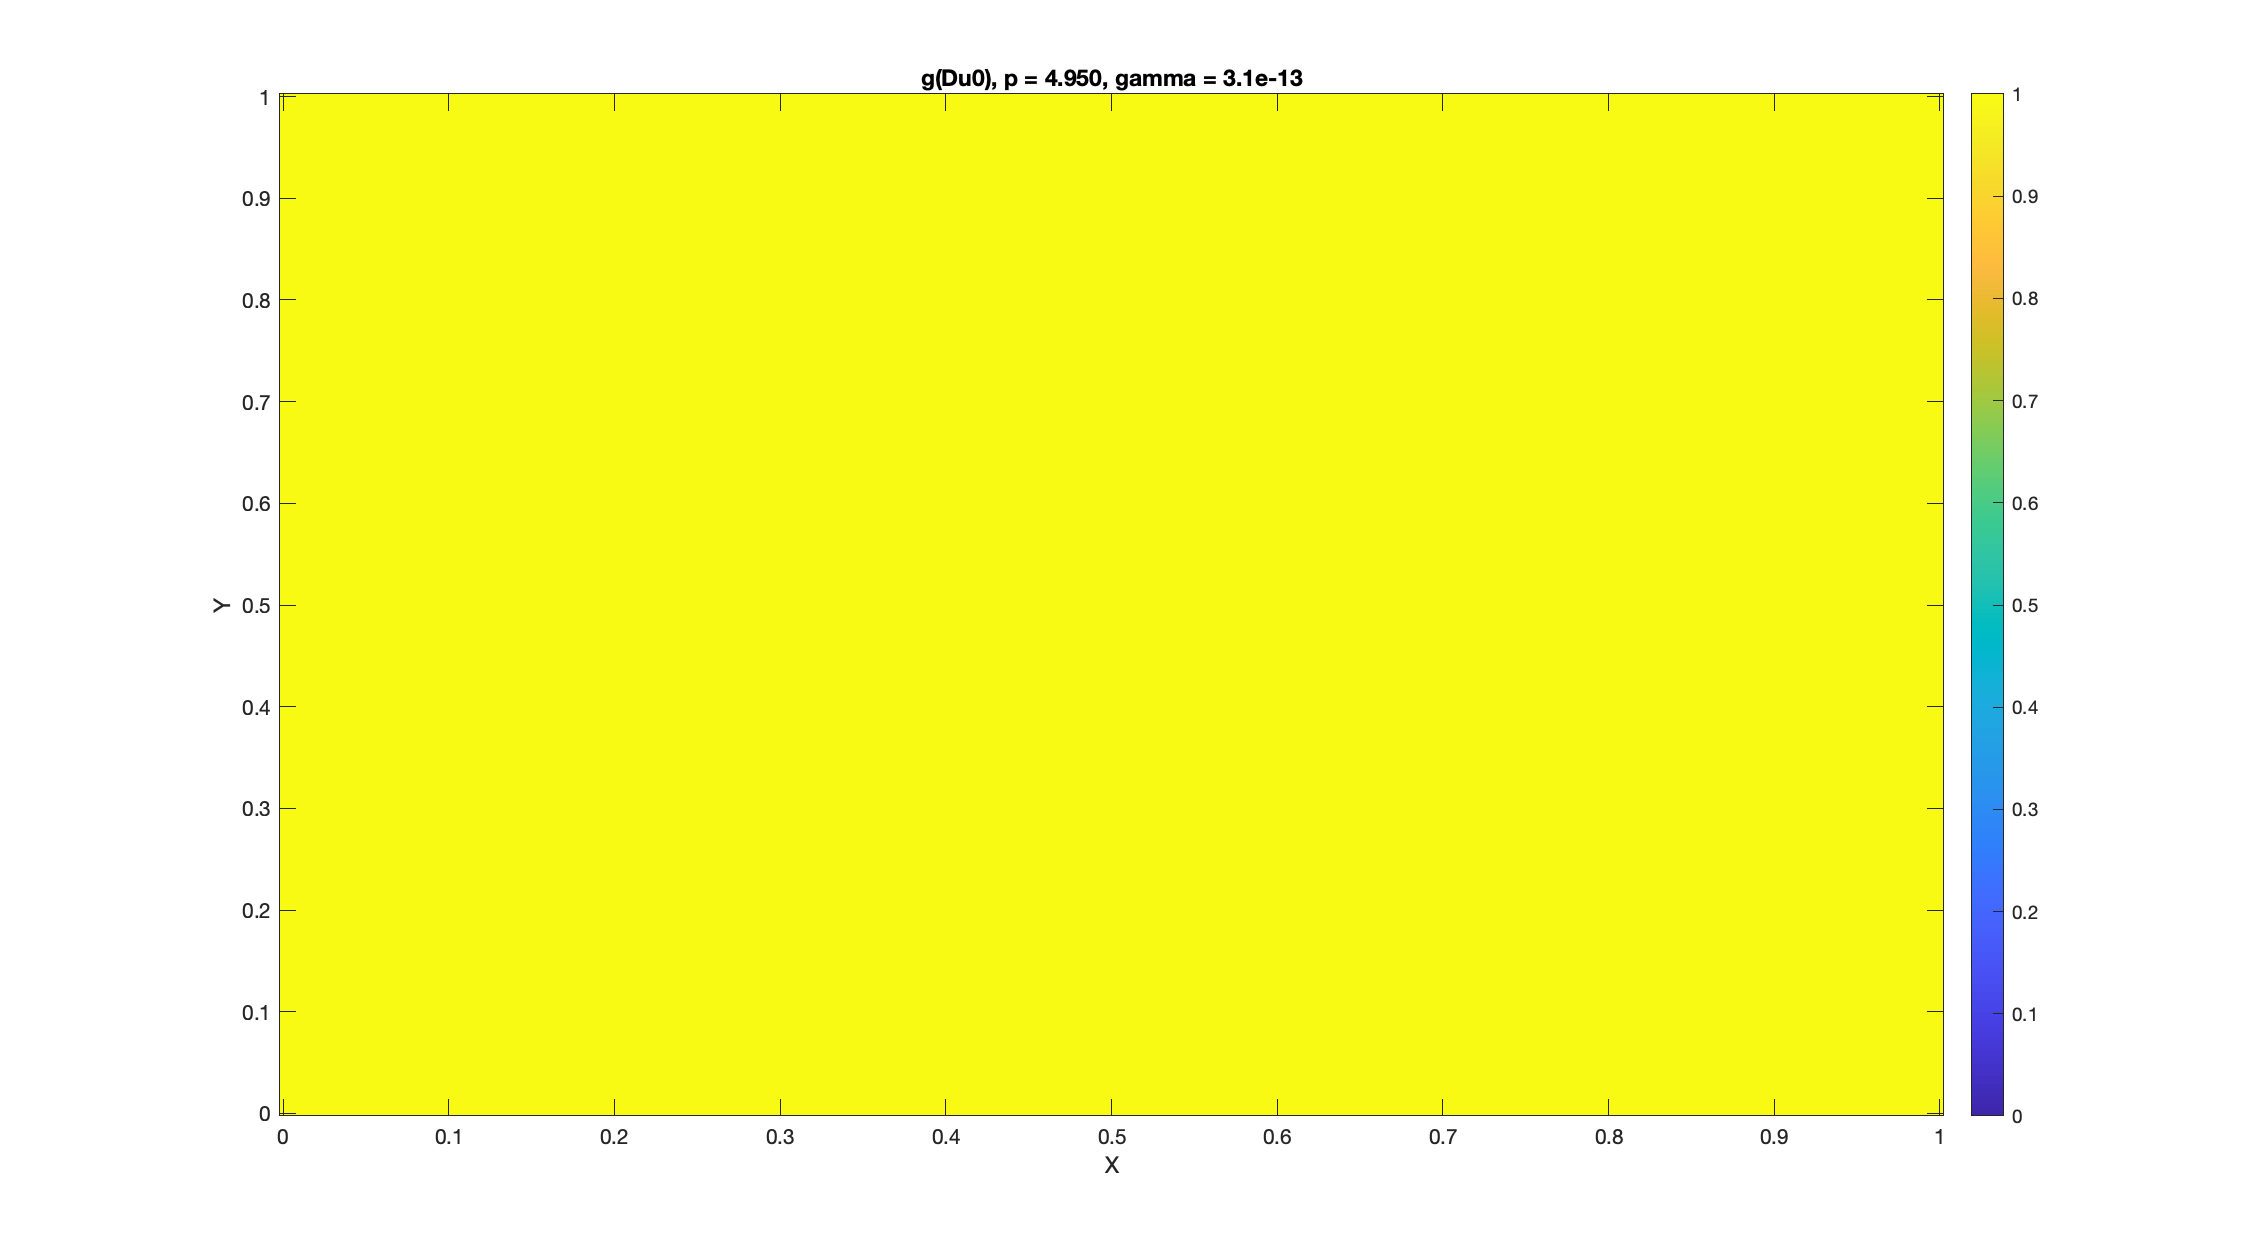
\includegraphics[width=0.5\textwidth]{ex2spd.png}}
  \\
  \subfloat[]{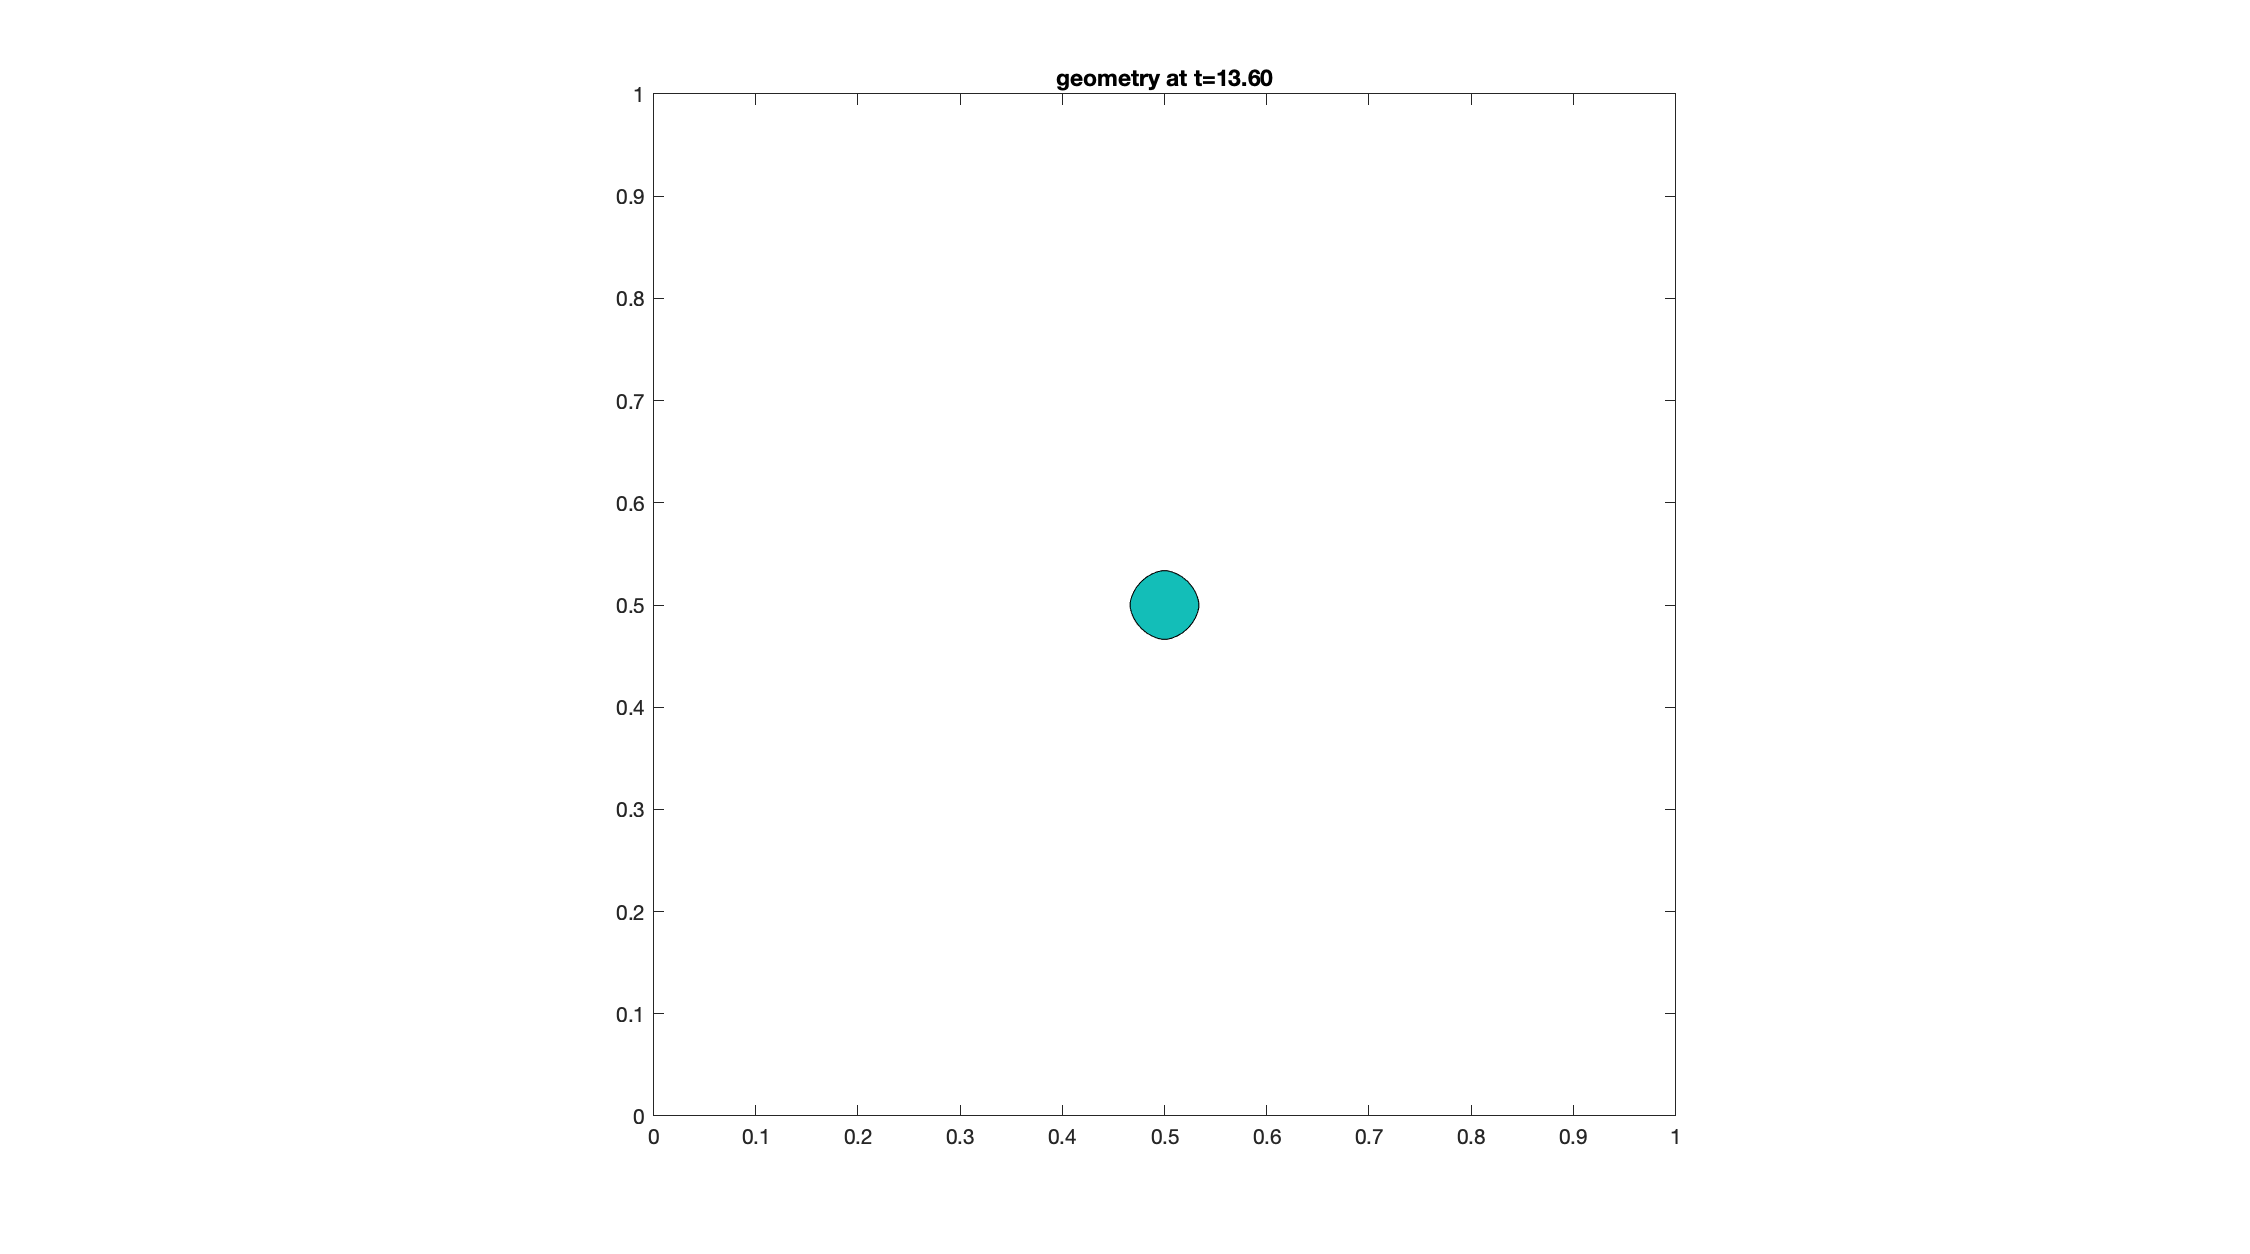
\includegraphics[width=0.5\textwidth]{ex2final.png}}
  \caption{$\sigma = 6.5\times 10^{-5}$, $p = 4.95$, $\gamma=5.5\times 10^{-13.25}$}
\end{figure}
The middle plot that is yellow indicates that the front will continue to move at speed 1; therefore, this parameter was too low for the front to ``detect'' the image contour. In the next example I double $p$
\clearpage
\begin{figure}[h!]
  \centering
  \subfloat[]{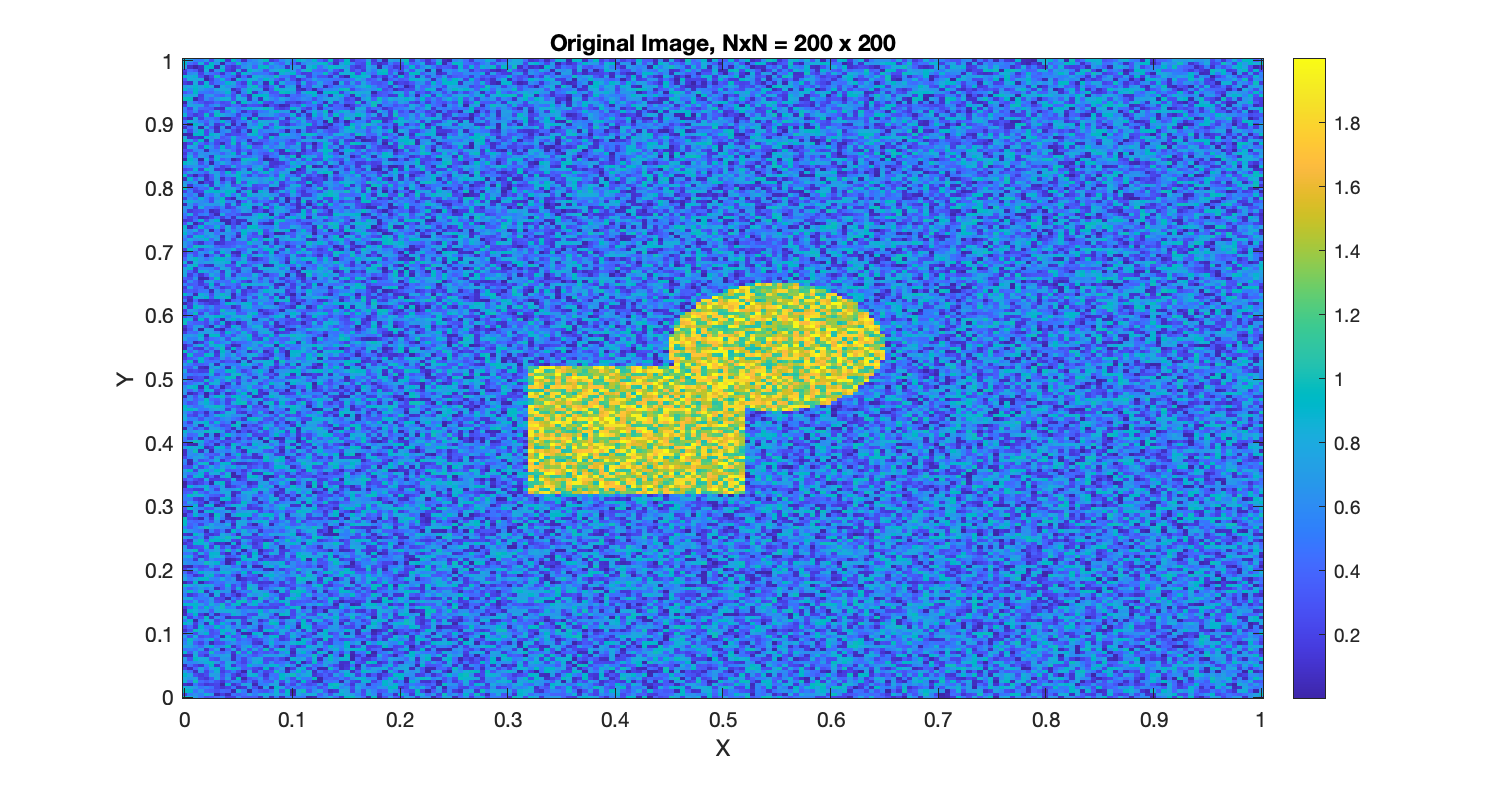
\includegraphics[width=0.5\textwidth]{ex3original.png}}
  \hfill
  \subfloat[]{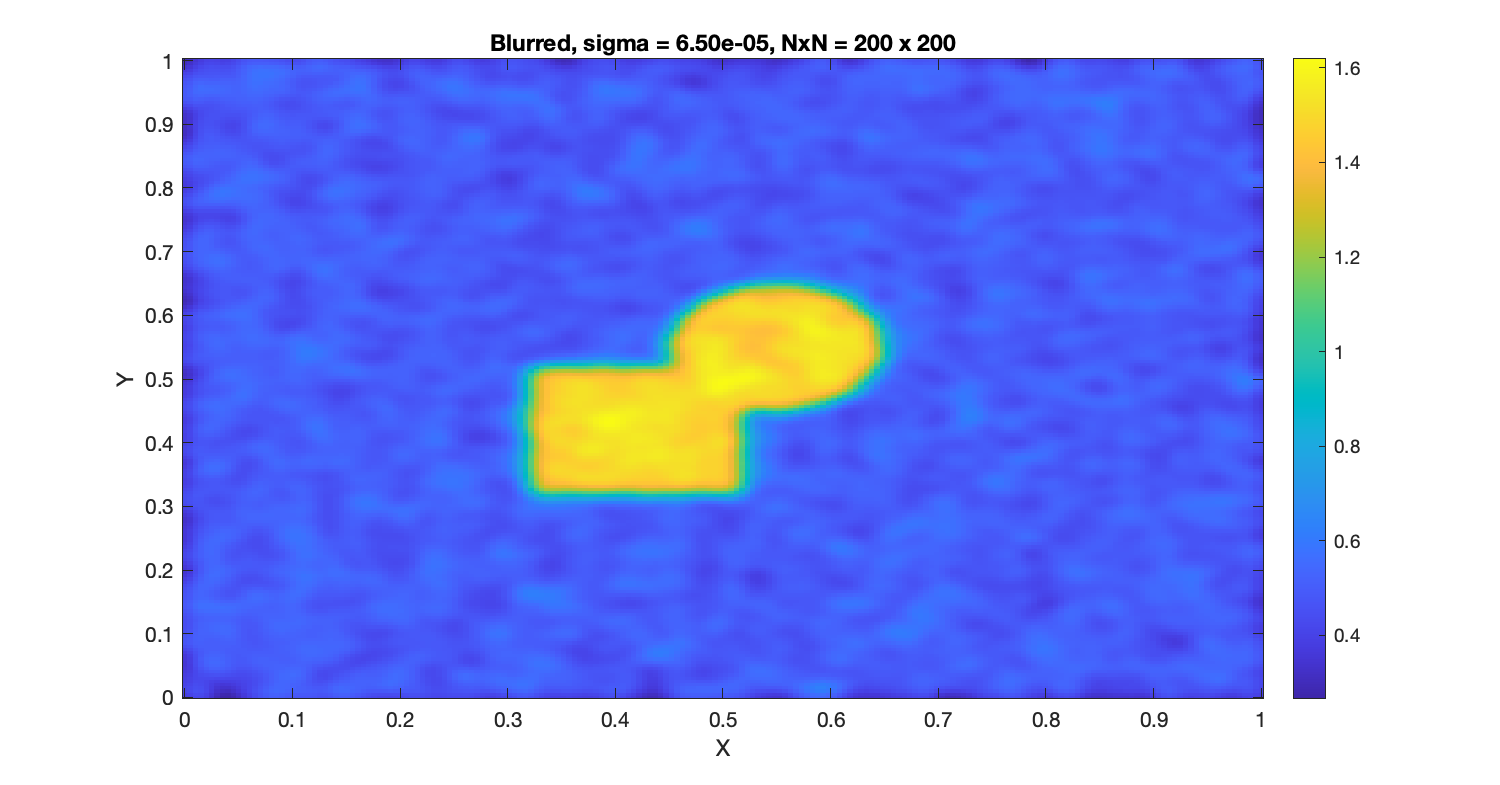
\includegraphics[width=0.5\textwidth]{ex3blurred.png}}\\
  \subfloat[]{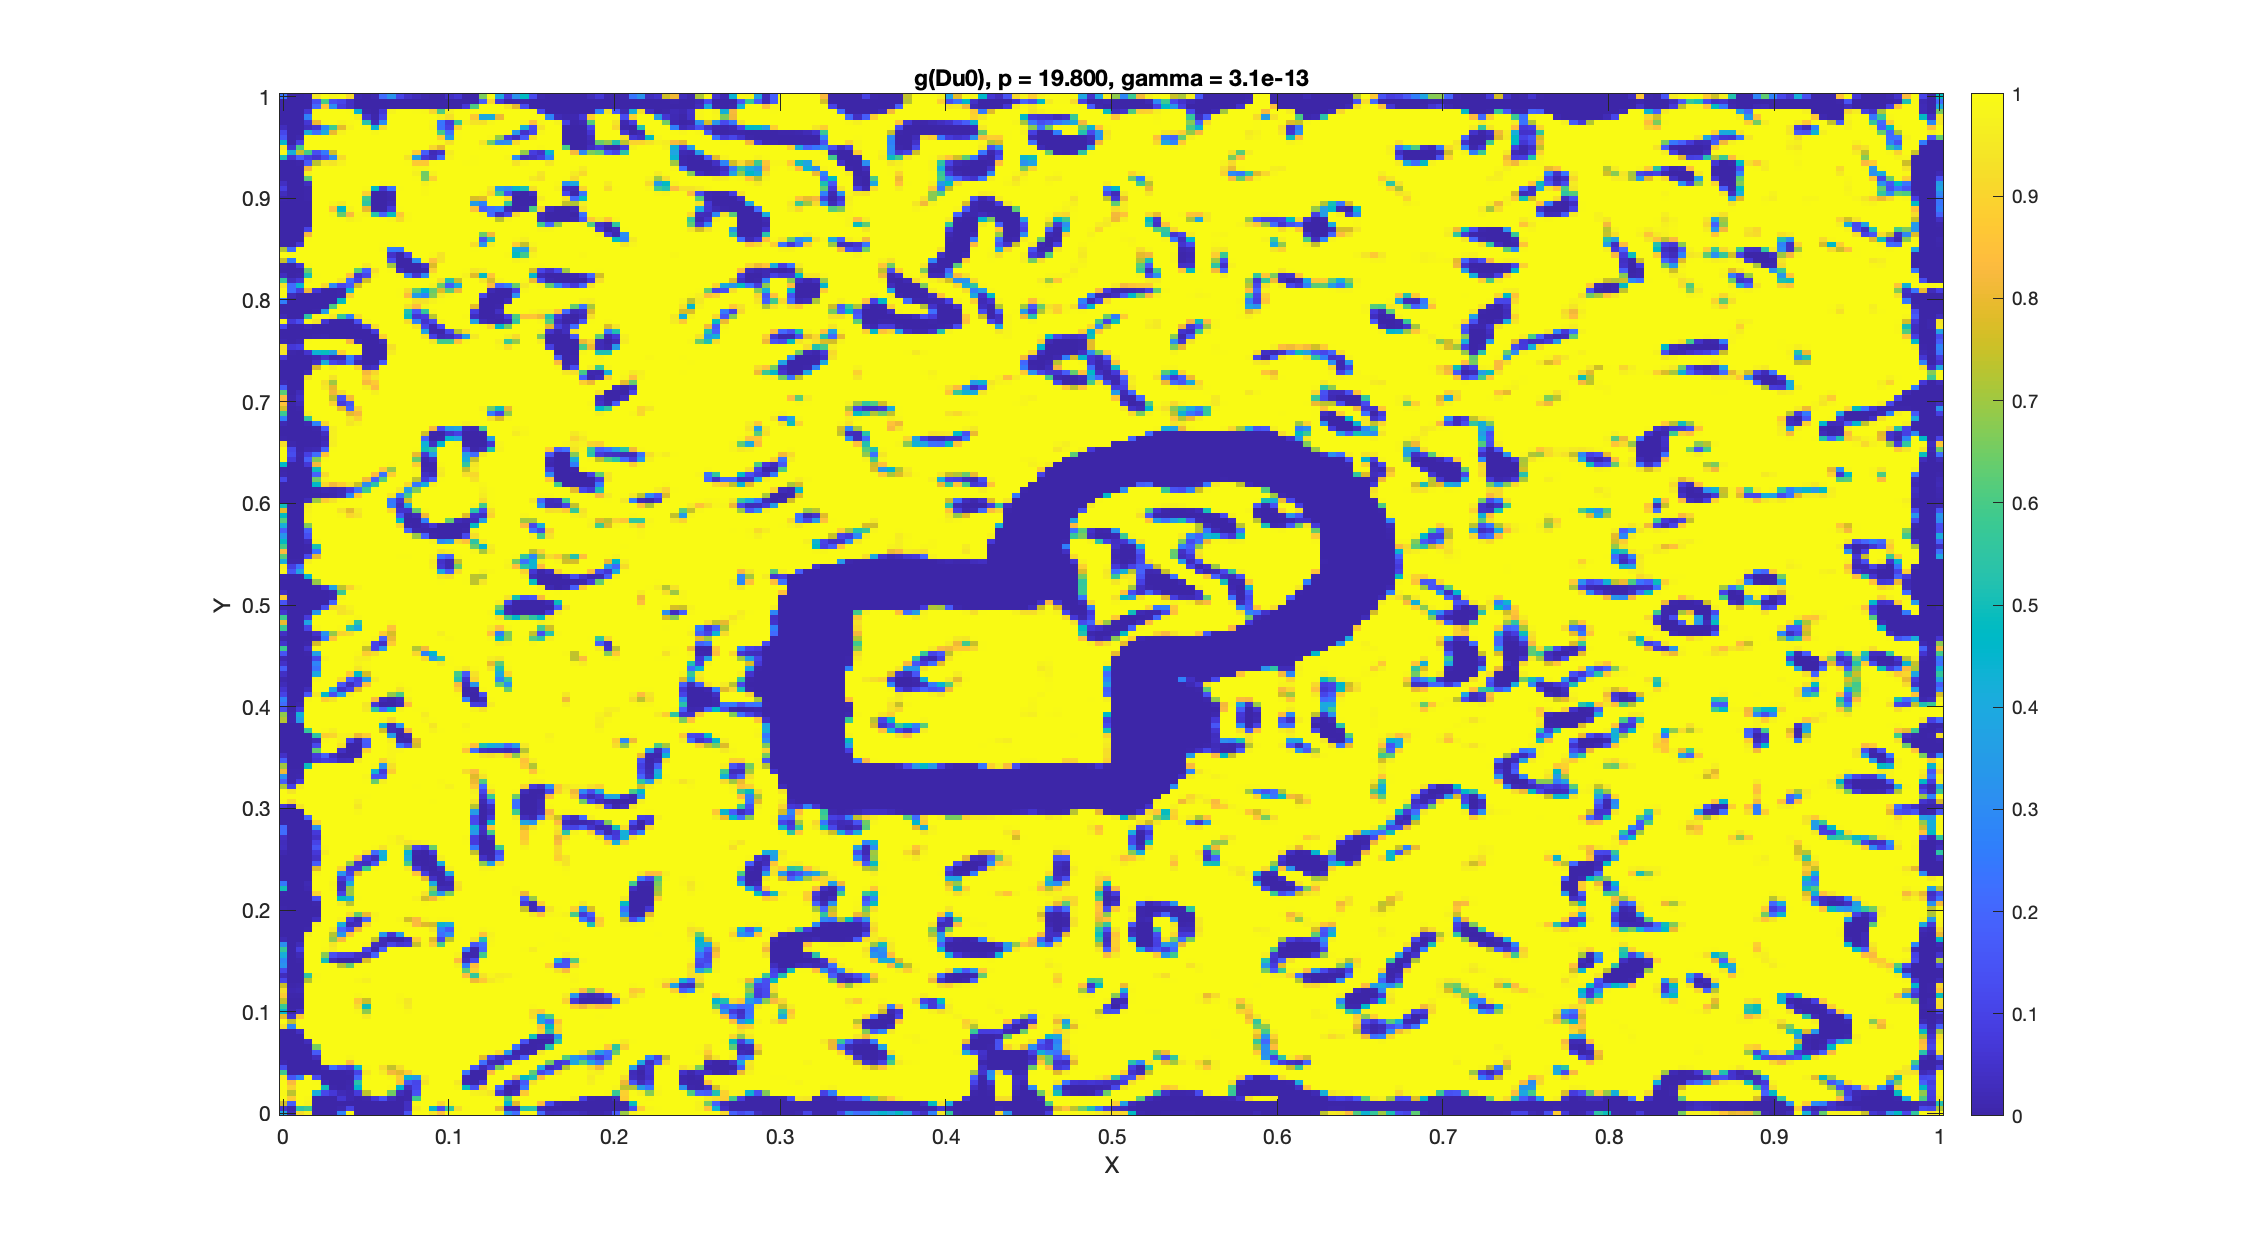
\includegraphics[width=0.5\textwidth]{ex3speedfunction_with_u0.png}}
  \\
  \subfloat[]{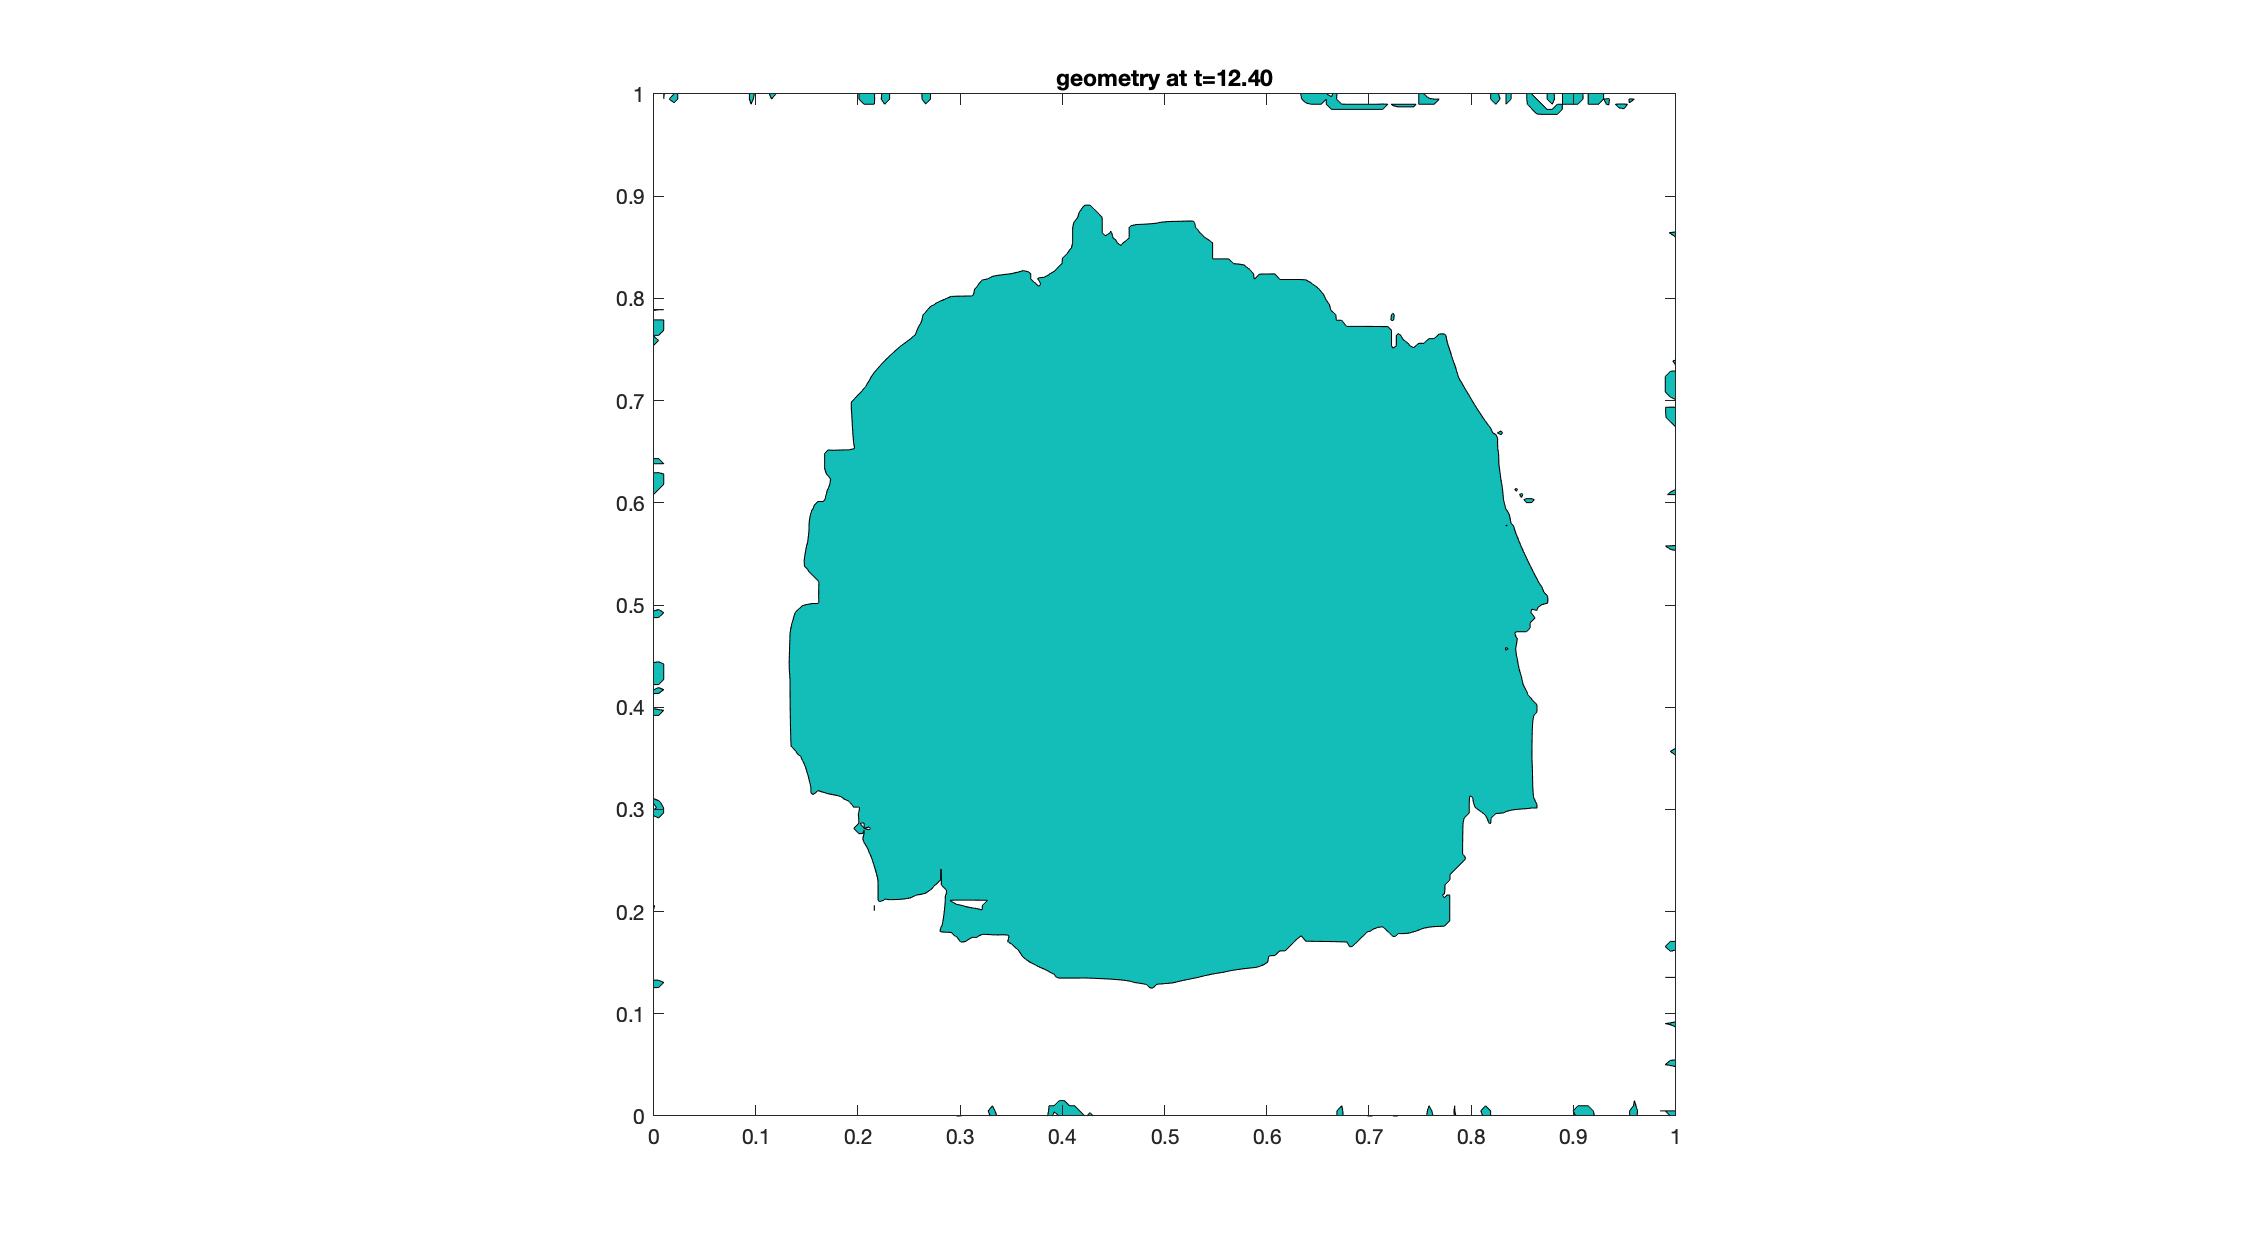
\includegraphics[width=0.5\textwidth]{ex3final.png}}
  \caption{$\sigma = 6.5\times 10^{-5}$, $p = 19.8$, $\gamma=5.5\times 10^{-13.25}$}
\end{figure}
For the example above, the gradients are enhanced, which causes the front to move erratically; that is some parts of the function move inward while some are moving outward. We also see artifacts appearing along the edges of the image.
\clearpage
For this example I fixed $p=9.9$ and multiplied $\gamma$ by 100:
\begin{figure}[h!]
  \centering
  \subfloat[]{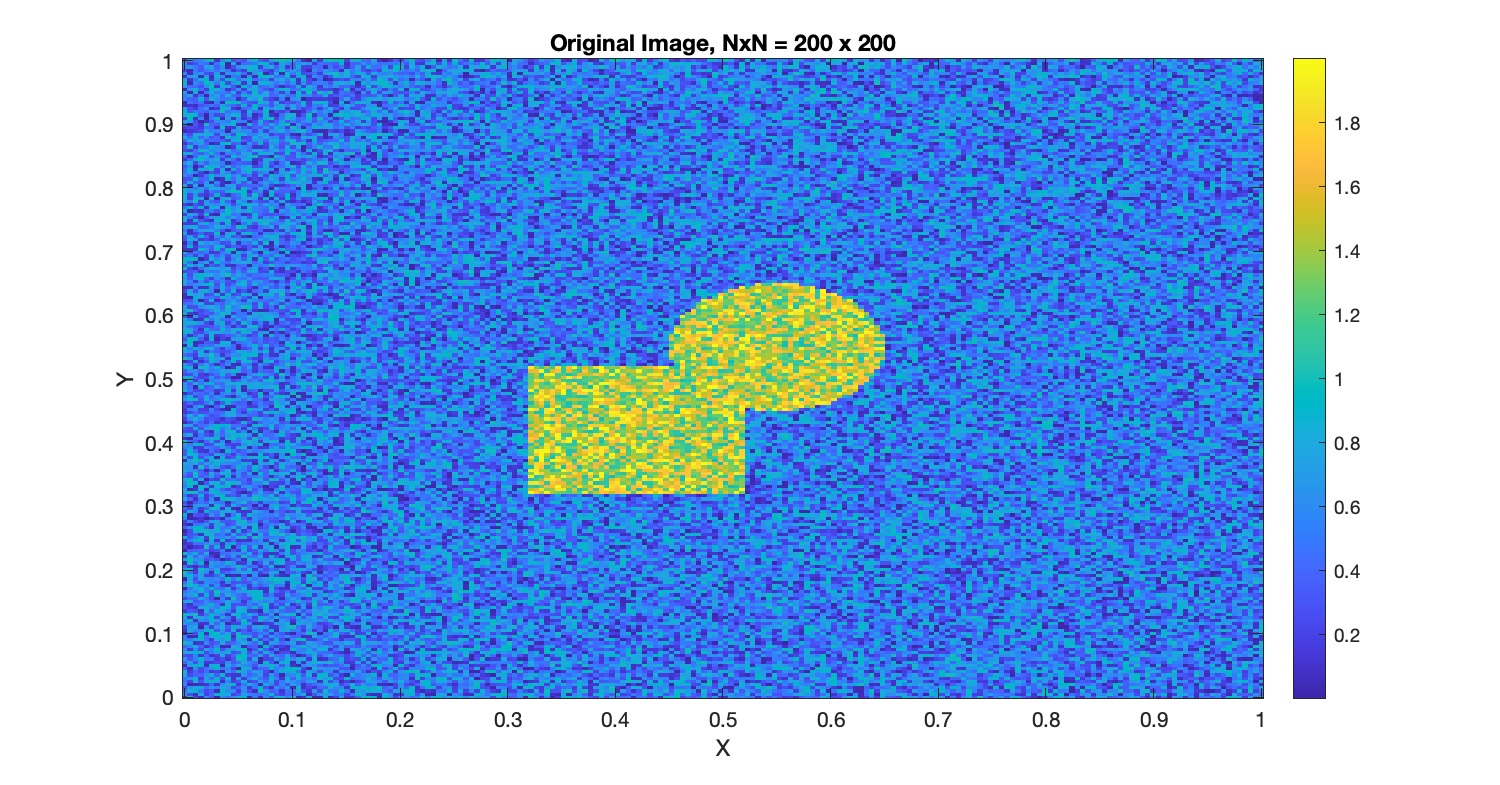
\includegraphics[width=0.5\textwidth]{ex4original.png}}
  \hfill
  \subfloat[]{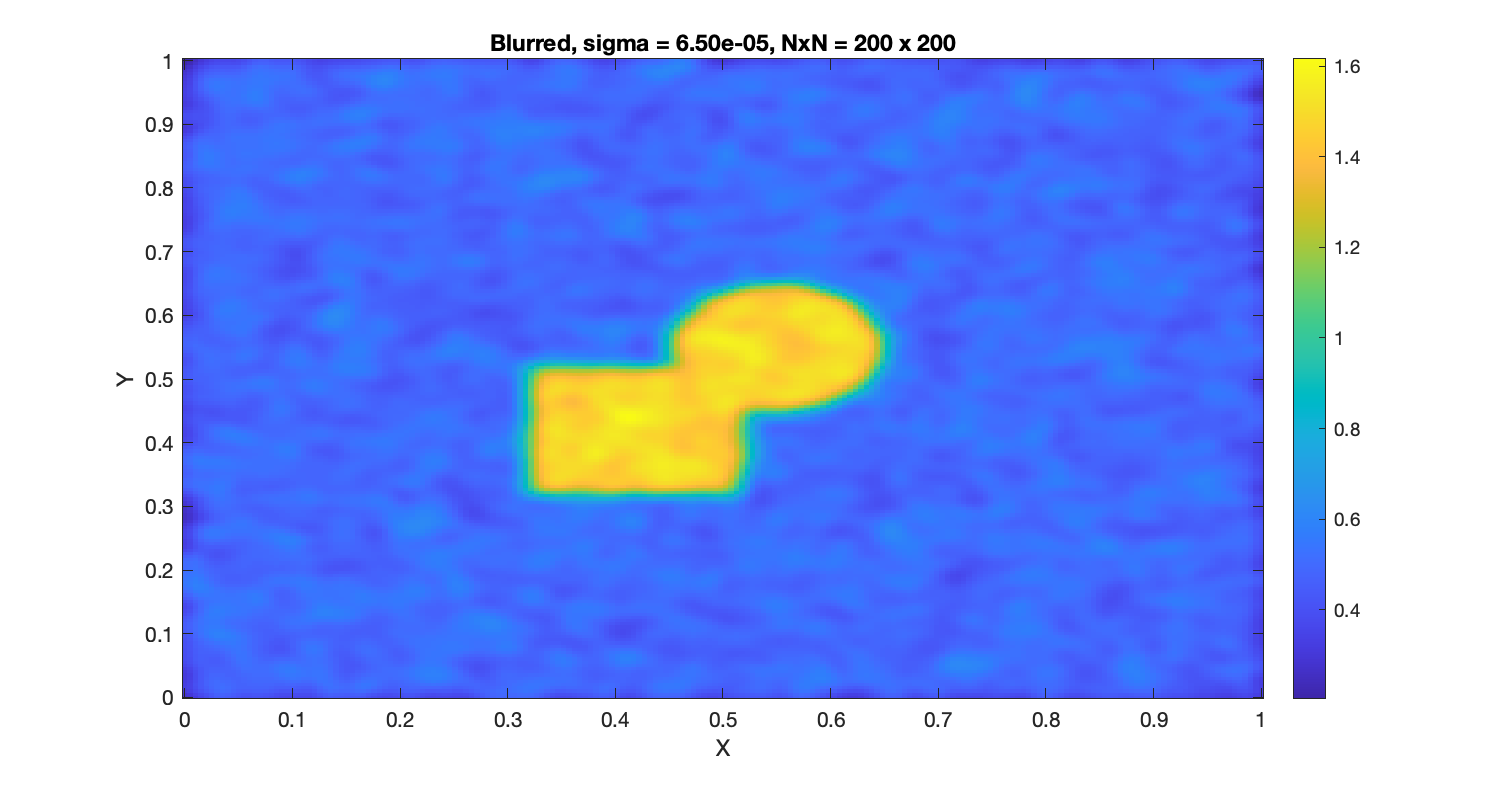
\includegraphics[width=0.5\textwidth]{ex4blurred.png}}\\
  \subfloat[]{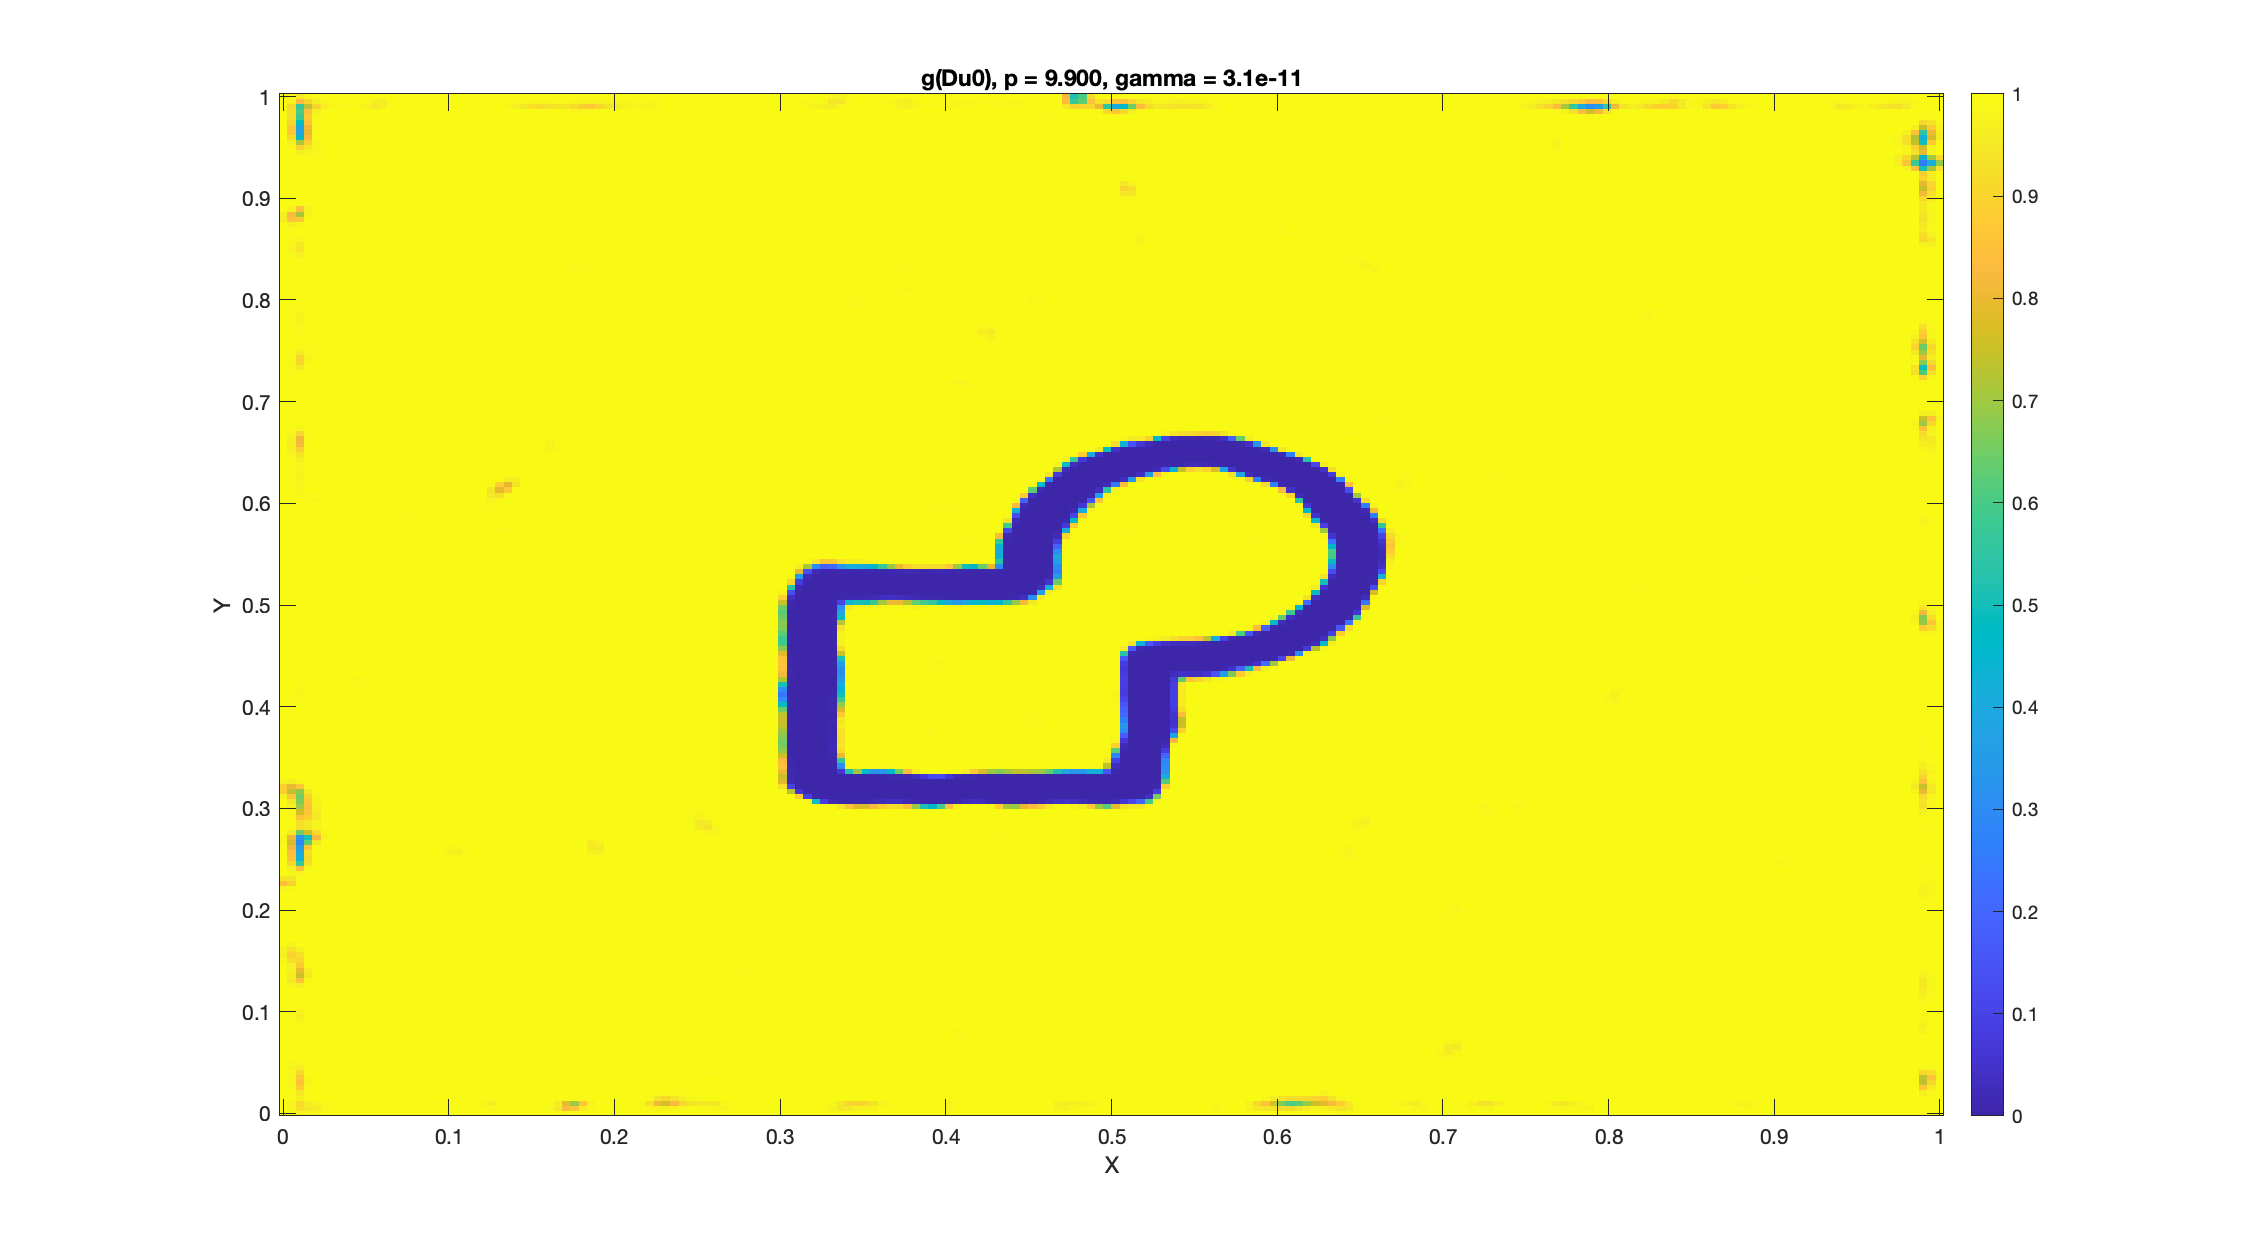
\includegraphics[width=0.5\textwidth]{ex4speedfunction_with_u0.png}}
  \\
  \subfloat[]{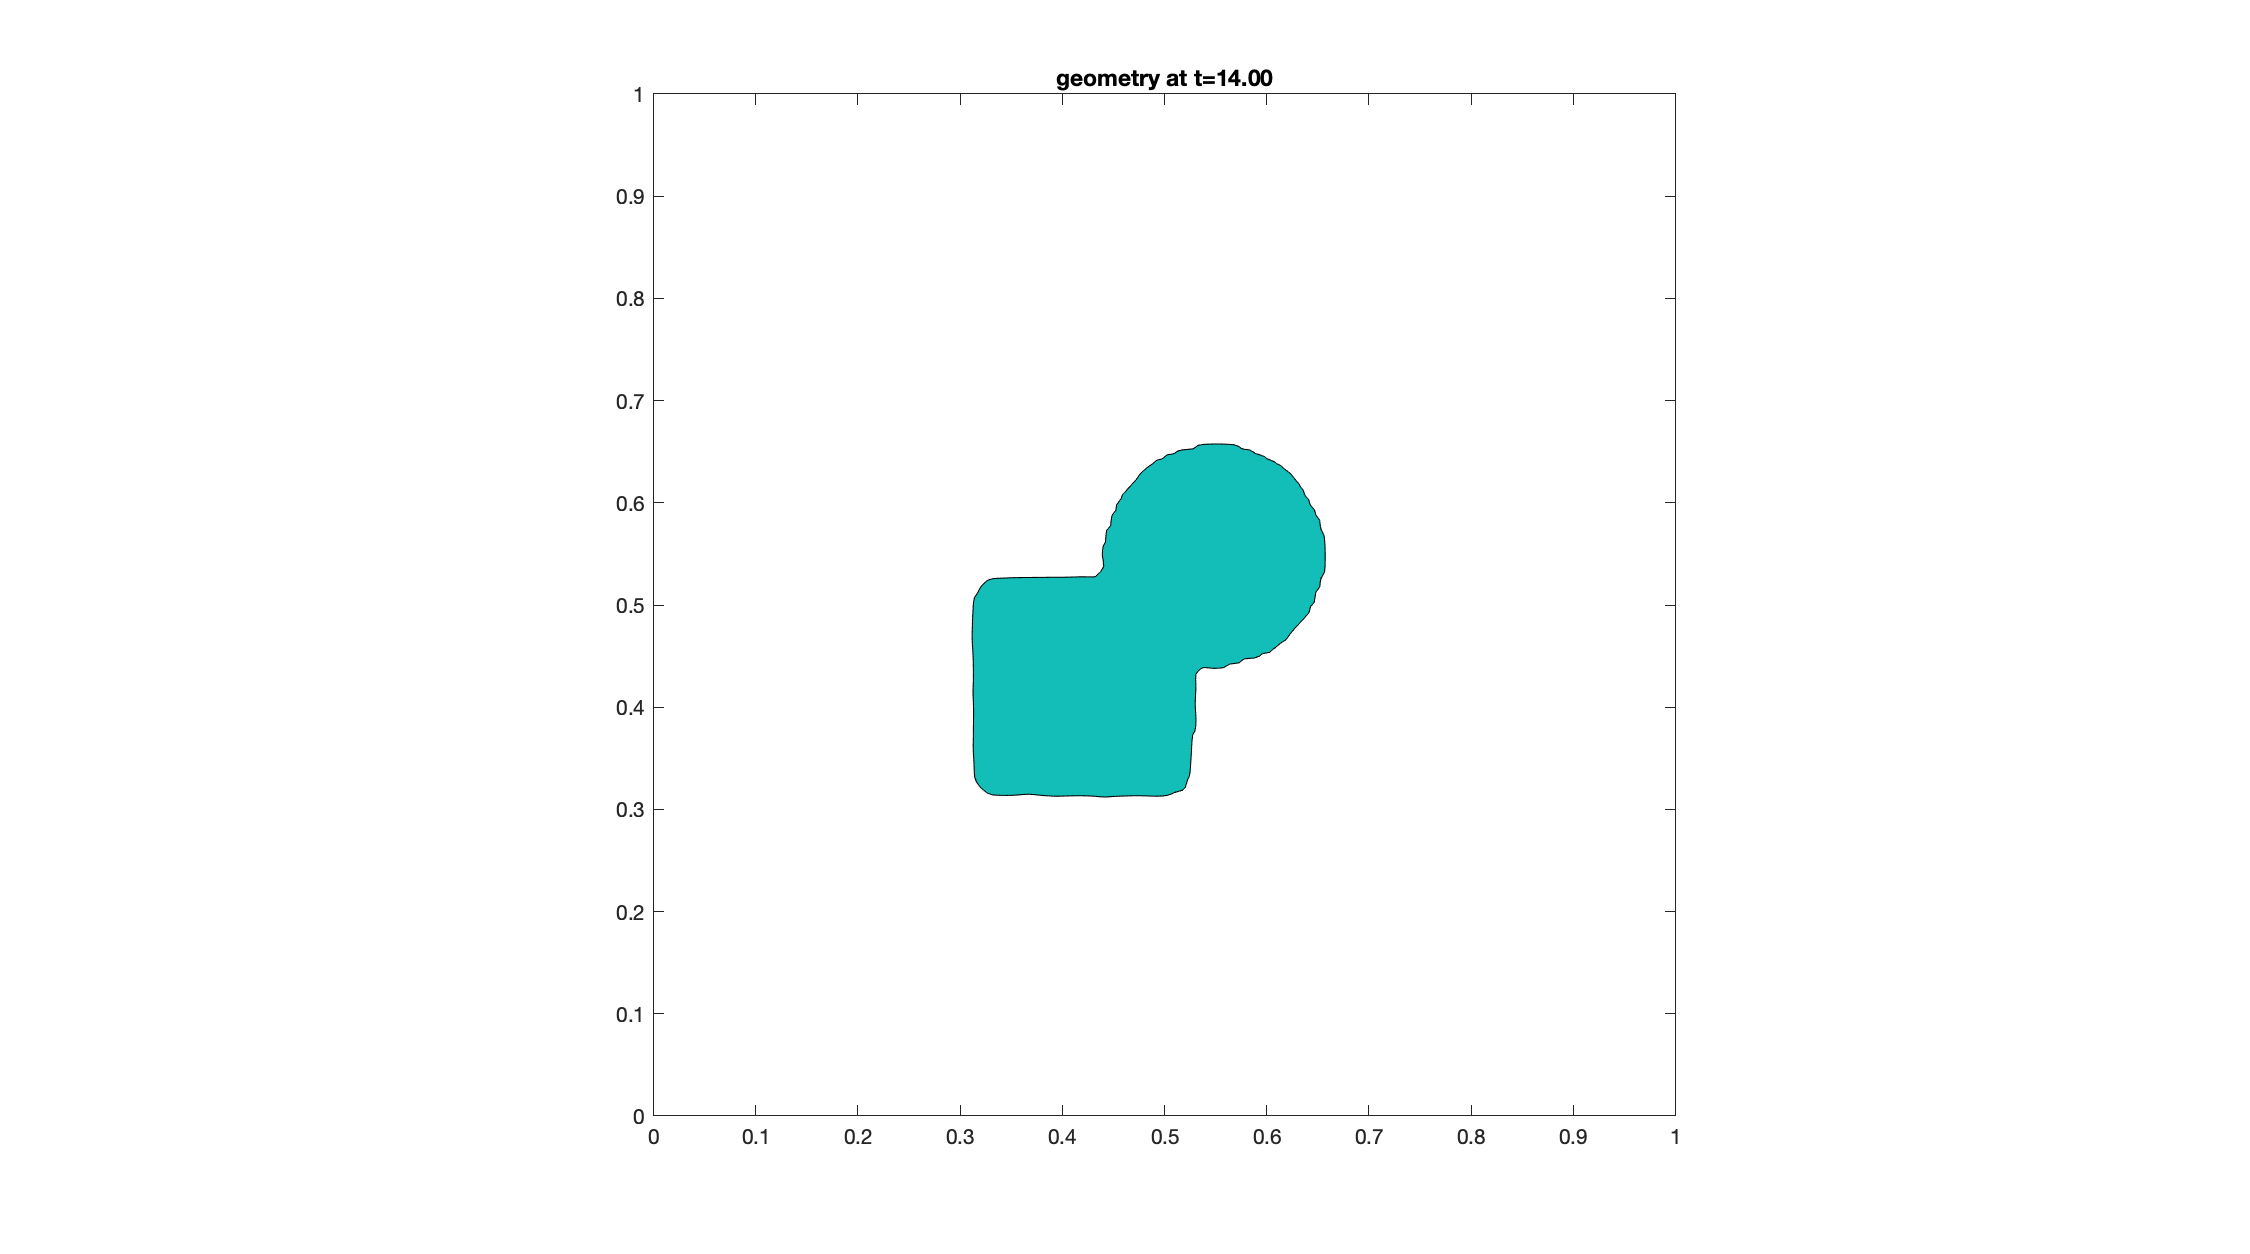
\includegraphics[width=0.5\textwidth]{ex4final.png}}
  \caption{$\sigma = 6.5\times 10^{-5}$, $p = 9.9$, $\gamma=5.5\times 10^{-11.25}$}
\end{figure}
This caused a slight increase in the speed at noisey locations near the edge of the image, but the front still converged to the image.
\clearpage
\begin{figure}[h!]
  \centering
  \subfloat[]{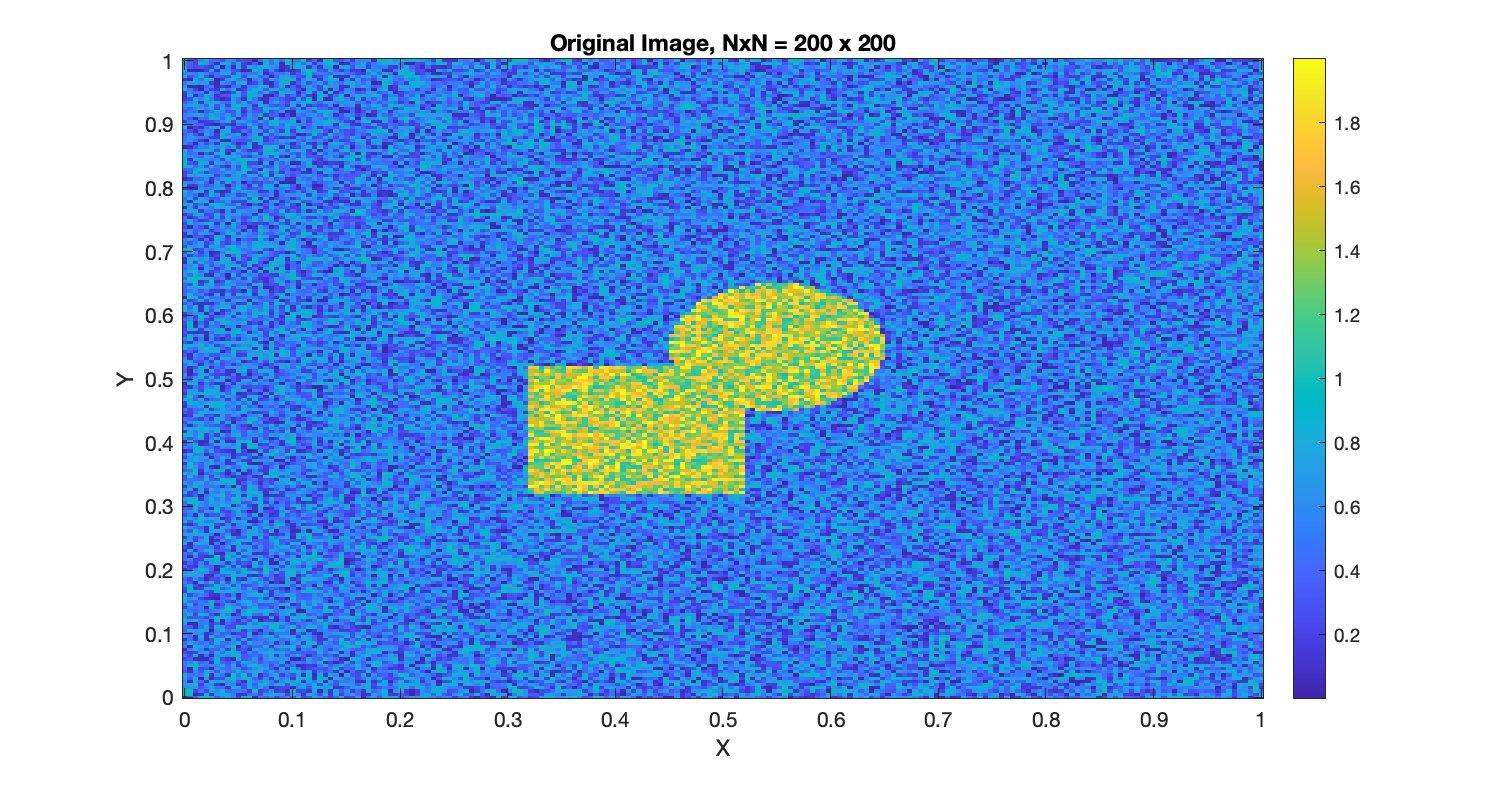
\includegraphics[width=0.5\textwidth]{ex5original.png}}
  \hfill
  \subfloat[]{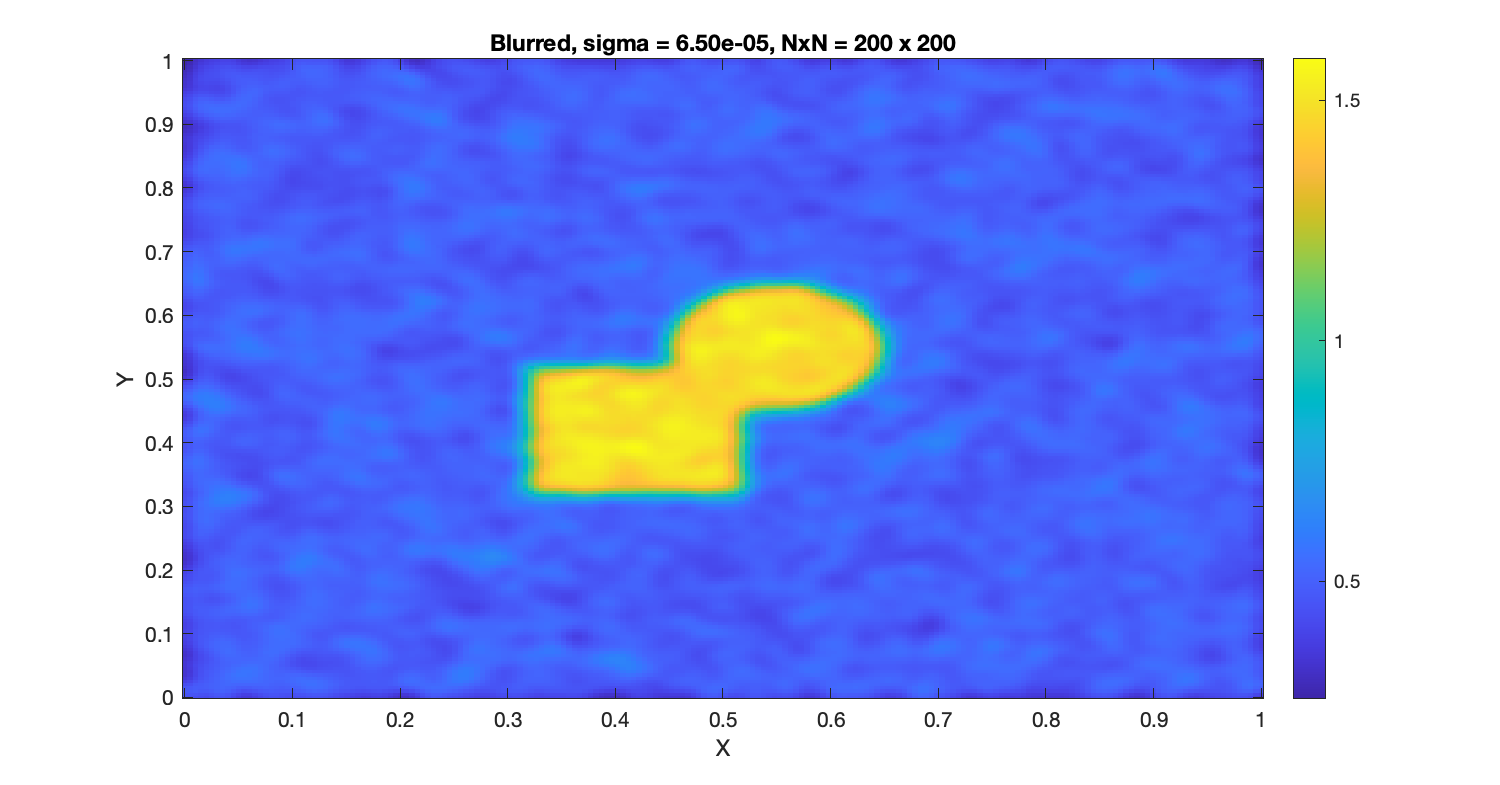
\includegraphics[width=0.5\textwidth]{ex5blurred.png}}\\
  \subfloat[]{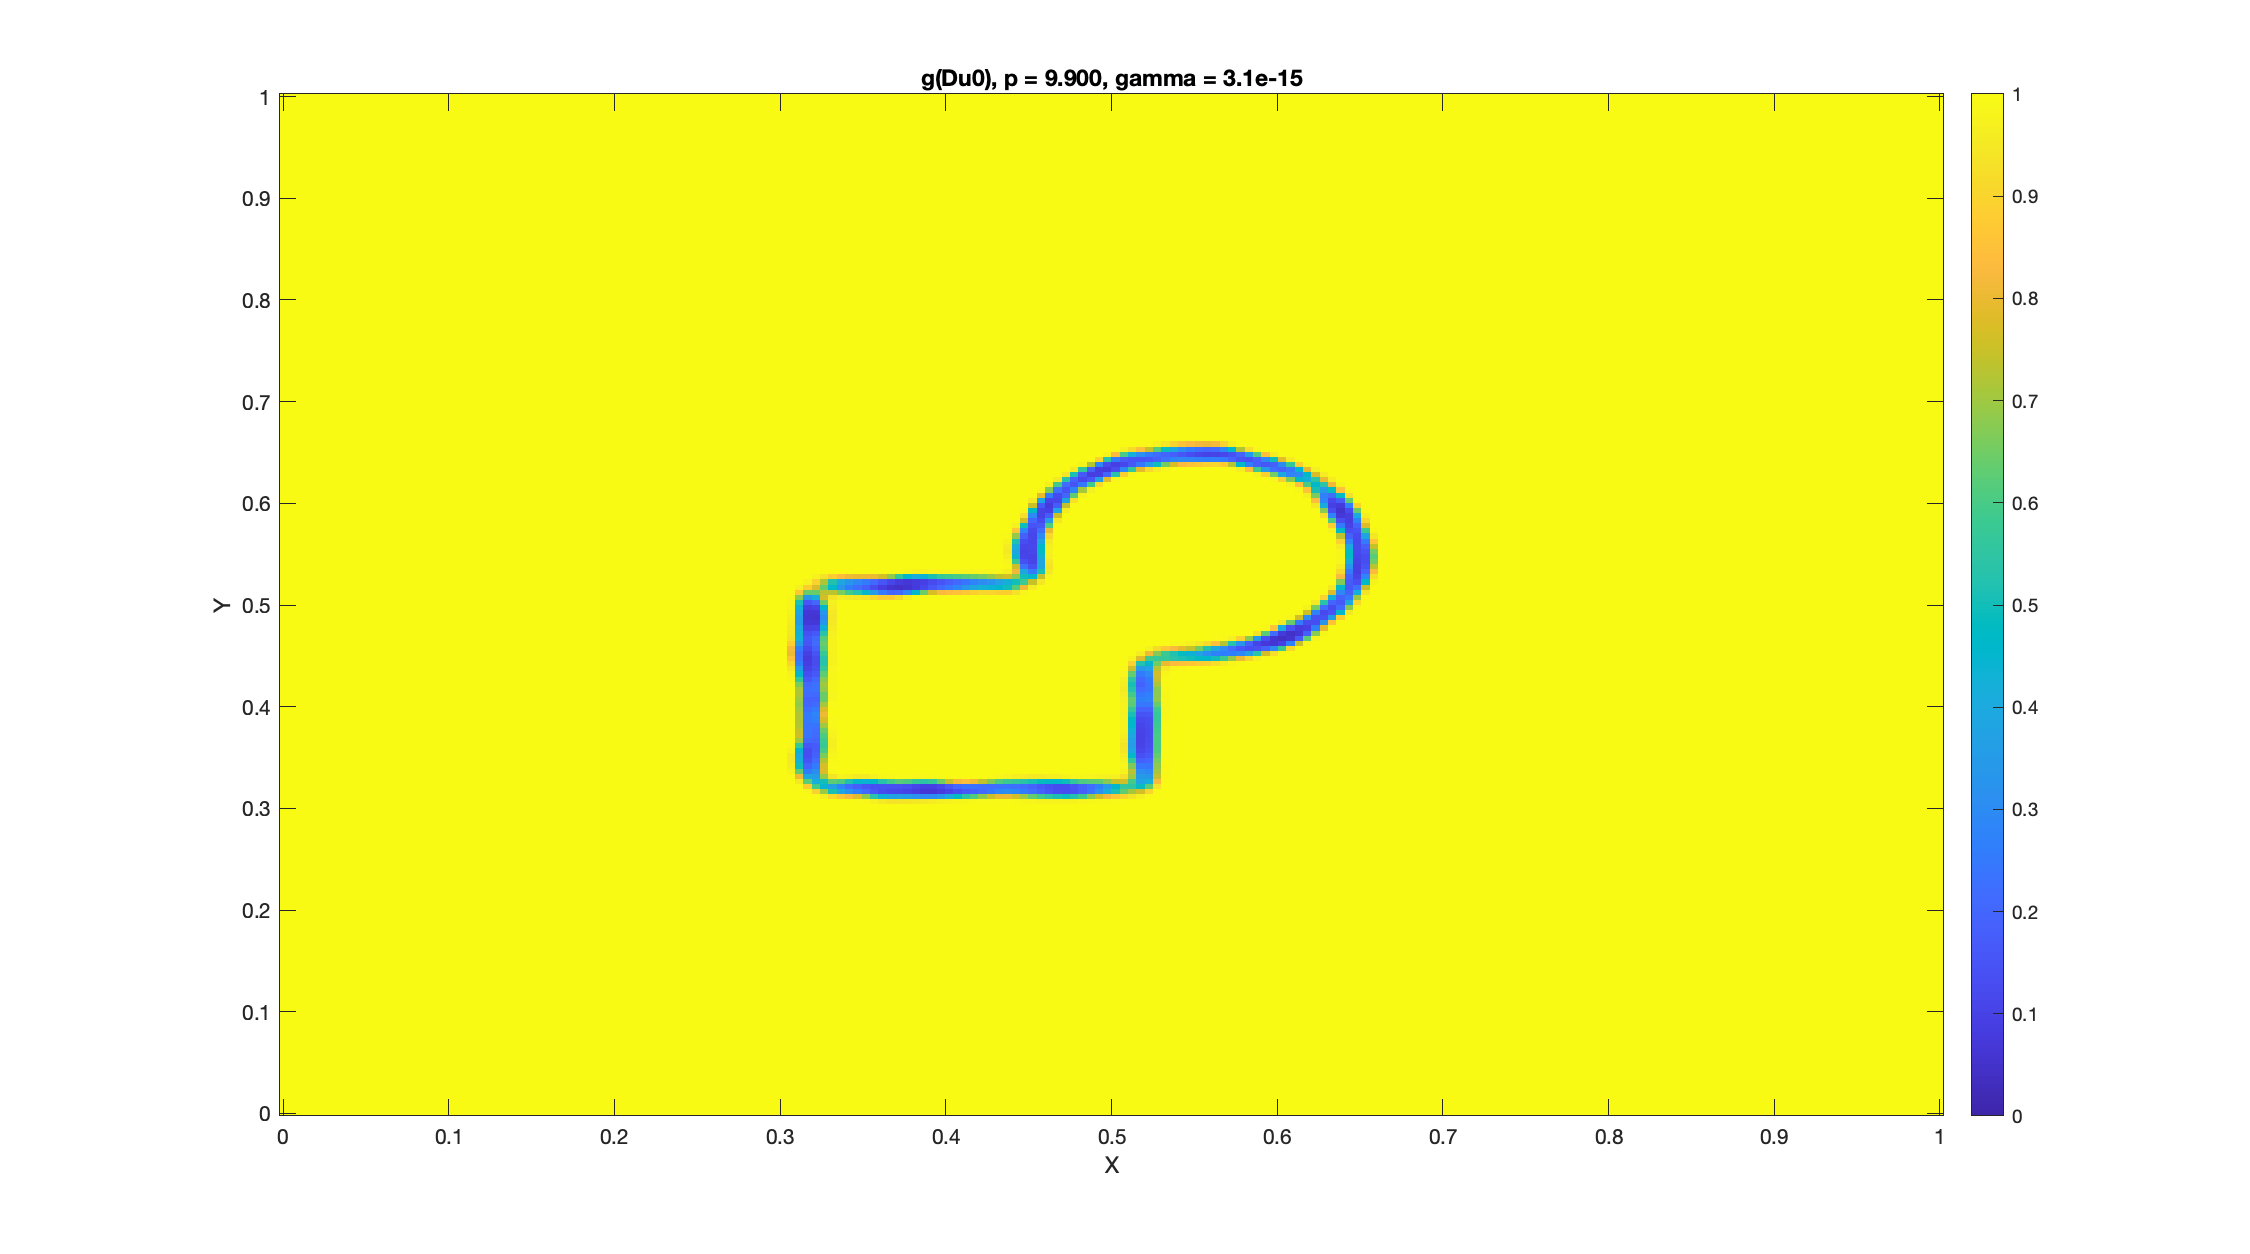
\includegraphics[width=0.5\textwidth]{ex5speedfunction_with_u0.png}}
  \\
  \subfloat[]{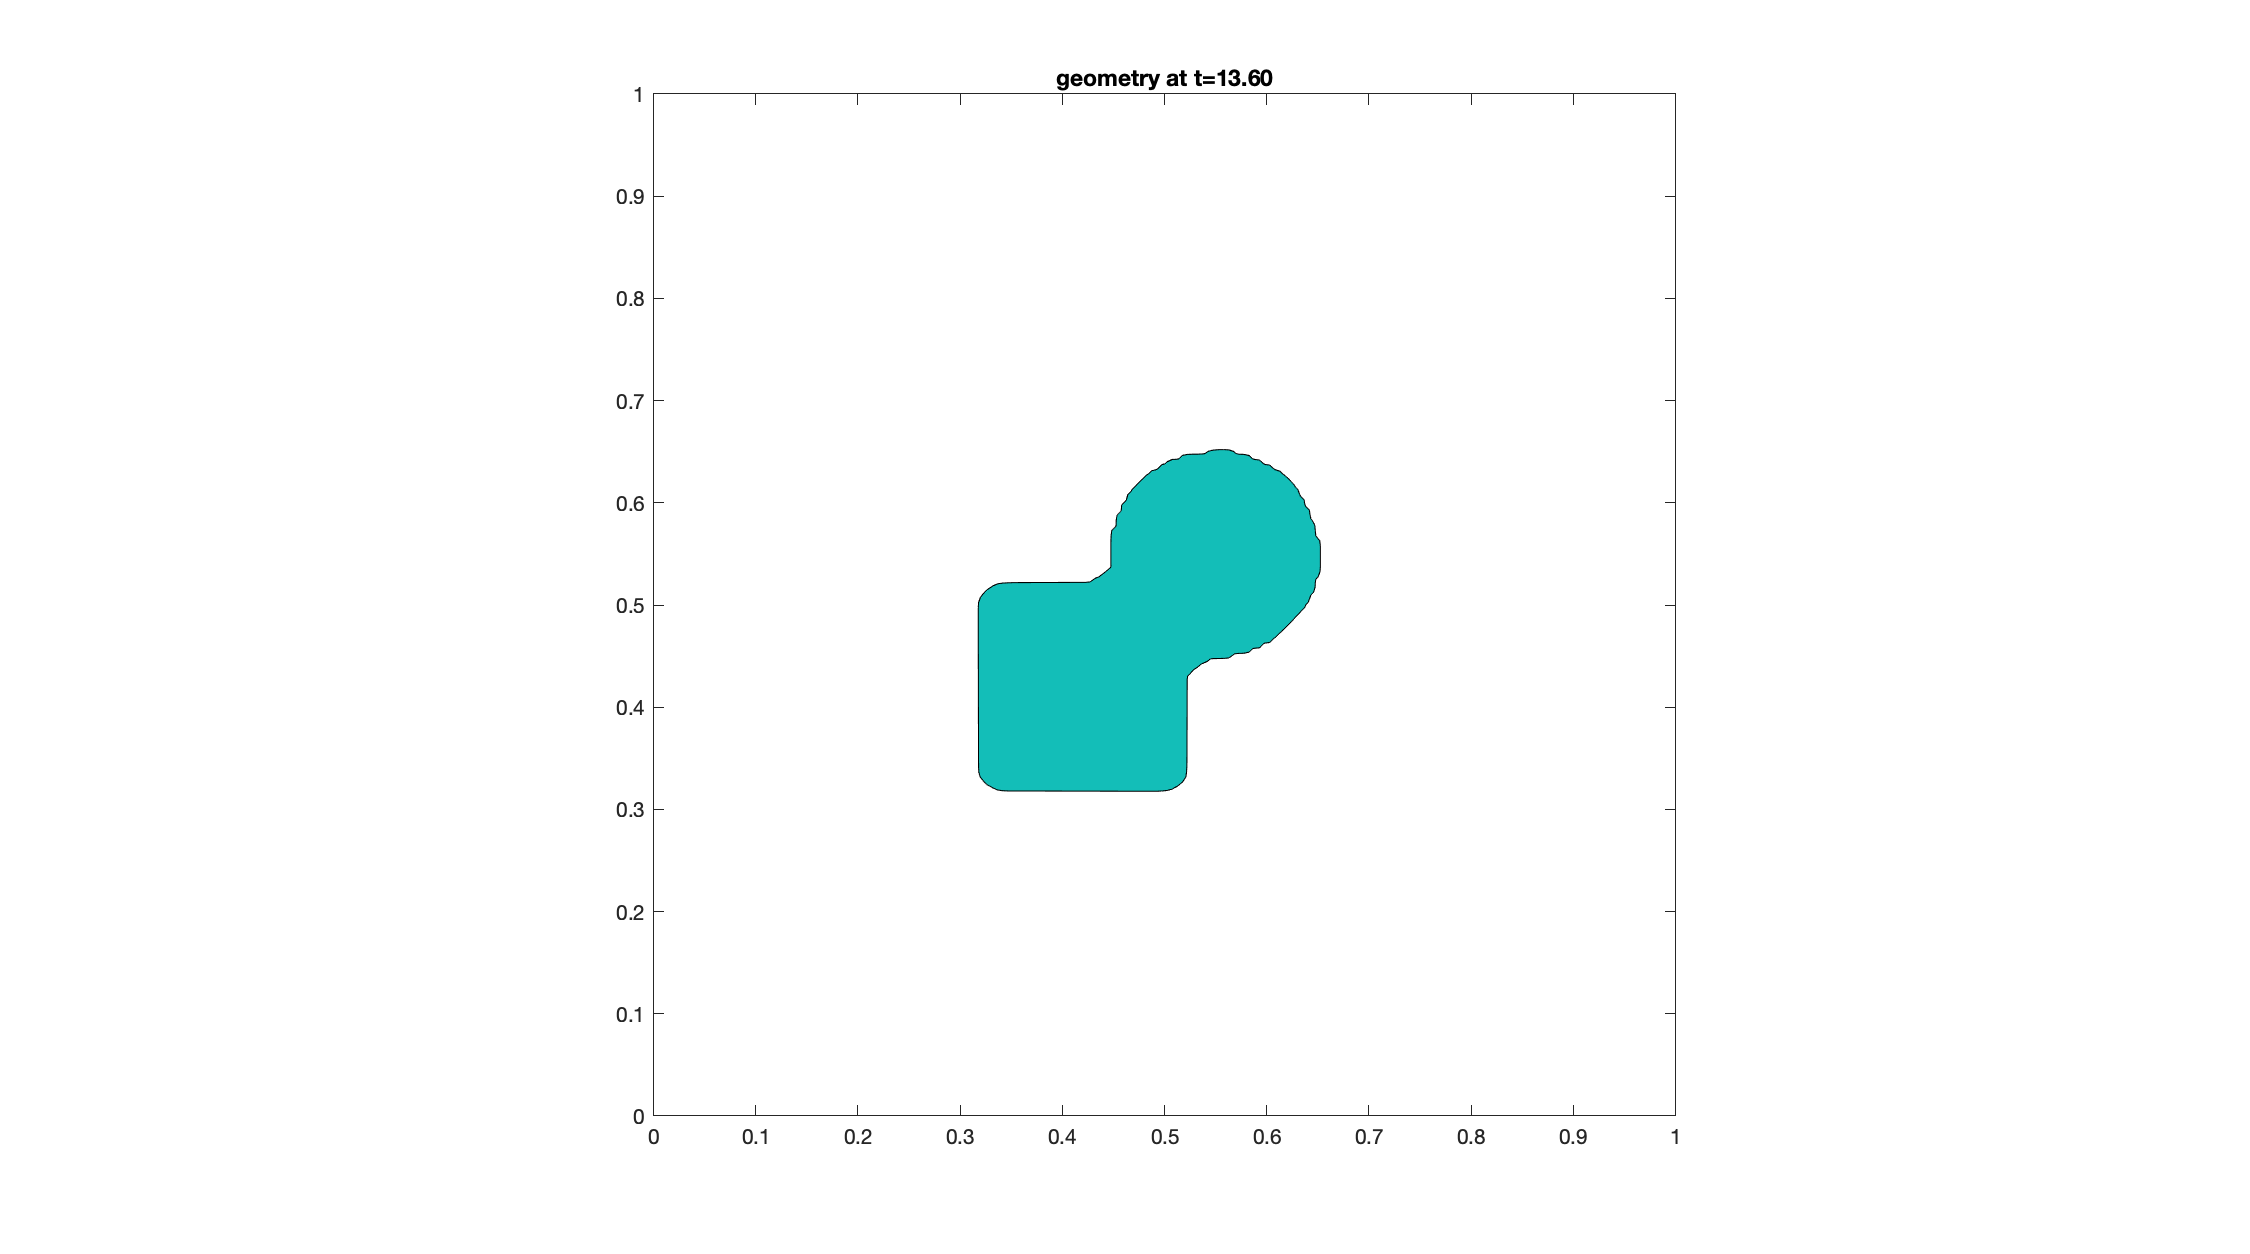
\includegraphics[width=0.5\textwidth]{ex5final.png}}
  \caption{$\sigma = 6.5\times 10^{-5}$, $p = 9.9$, $\gamma=5.5\times 10^{-15.25}$}
\end{figure}
In this example I divided $\gamma$ by a factor of 100. The speed increased at the interface of the image; however the image still converged and did not `pass' through. I also ran the code with more smoothing of the image, I doubled the variance: 
\clearpage
\begin{figure}[h!]
  \centering
  \subfloat[]{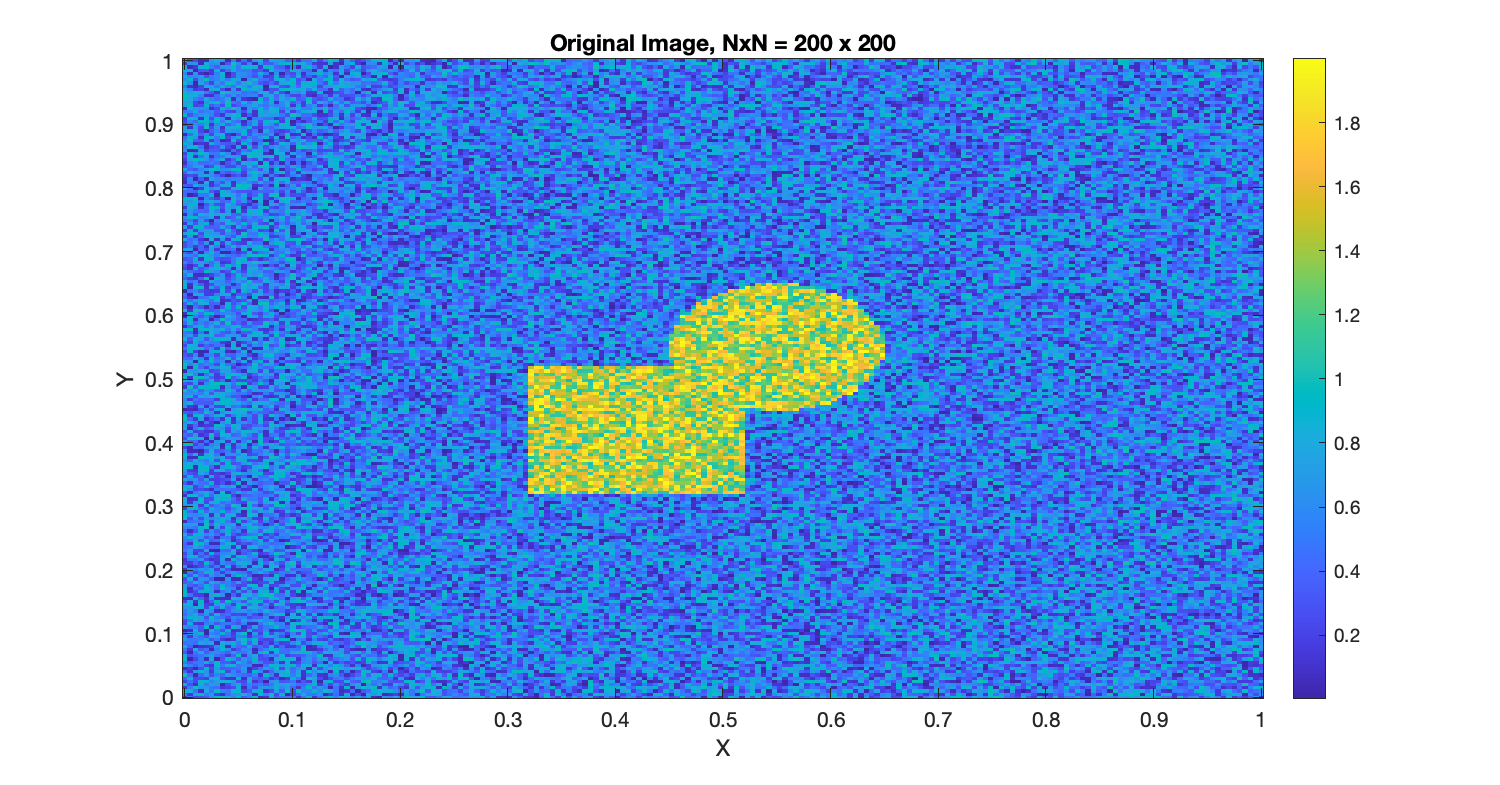
\includegraphics[width=0.5\textwidth]{ex6original.png}}
  \hfill
  \subfloat[]{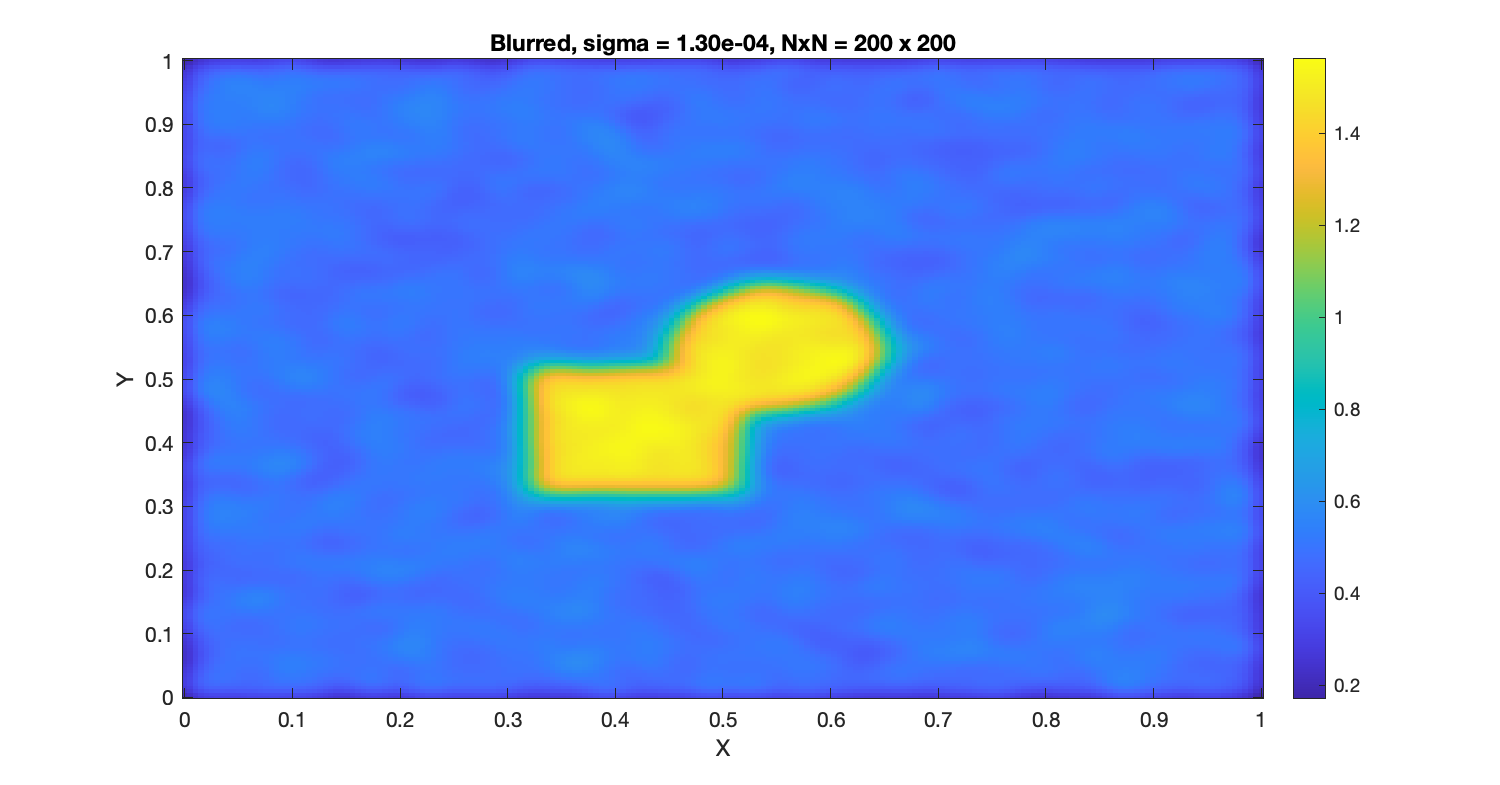
\includegraphics[width=0.5\textwidth]{ex6blurred.png}}\\
  \subfloat[]{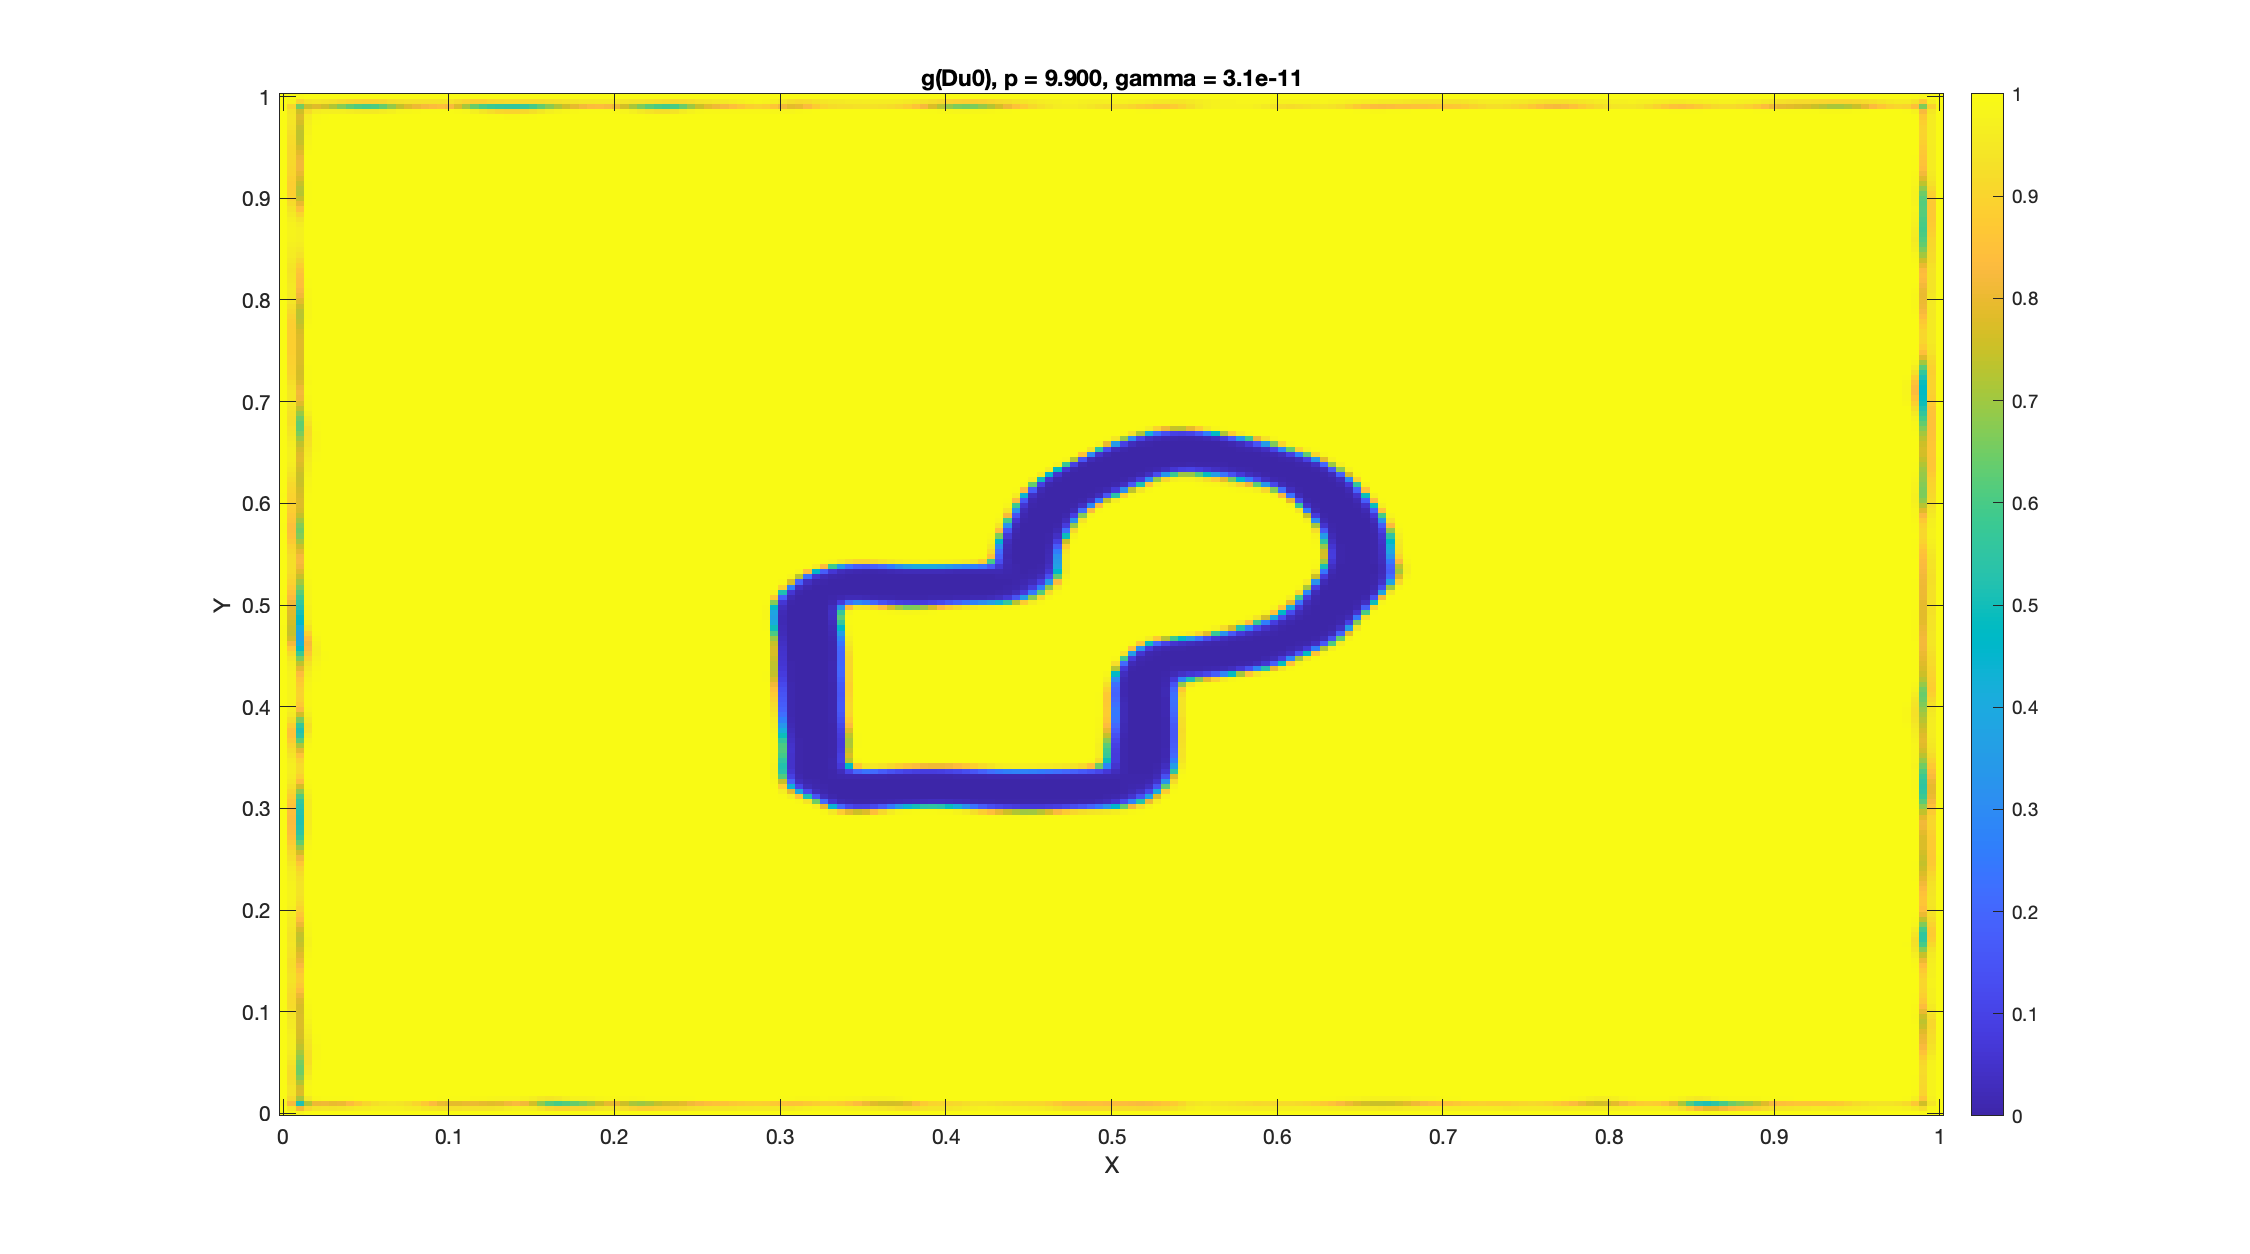
\includegraphics[width=0.5\textwidth]{ex6speedfunction_with_u0.png}}
  \\
  \subfloat[]{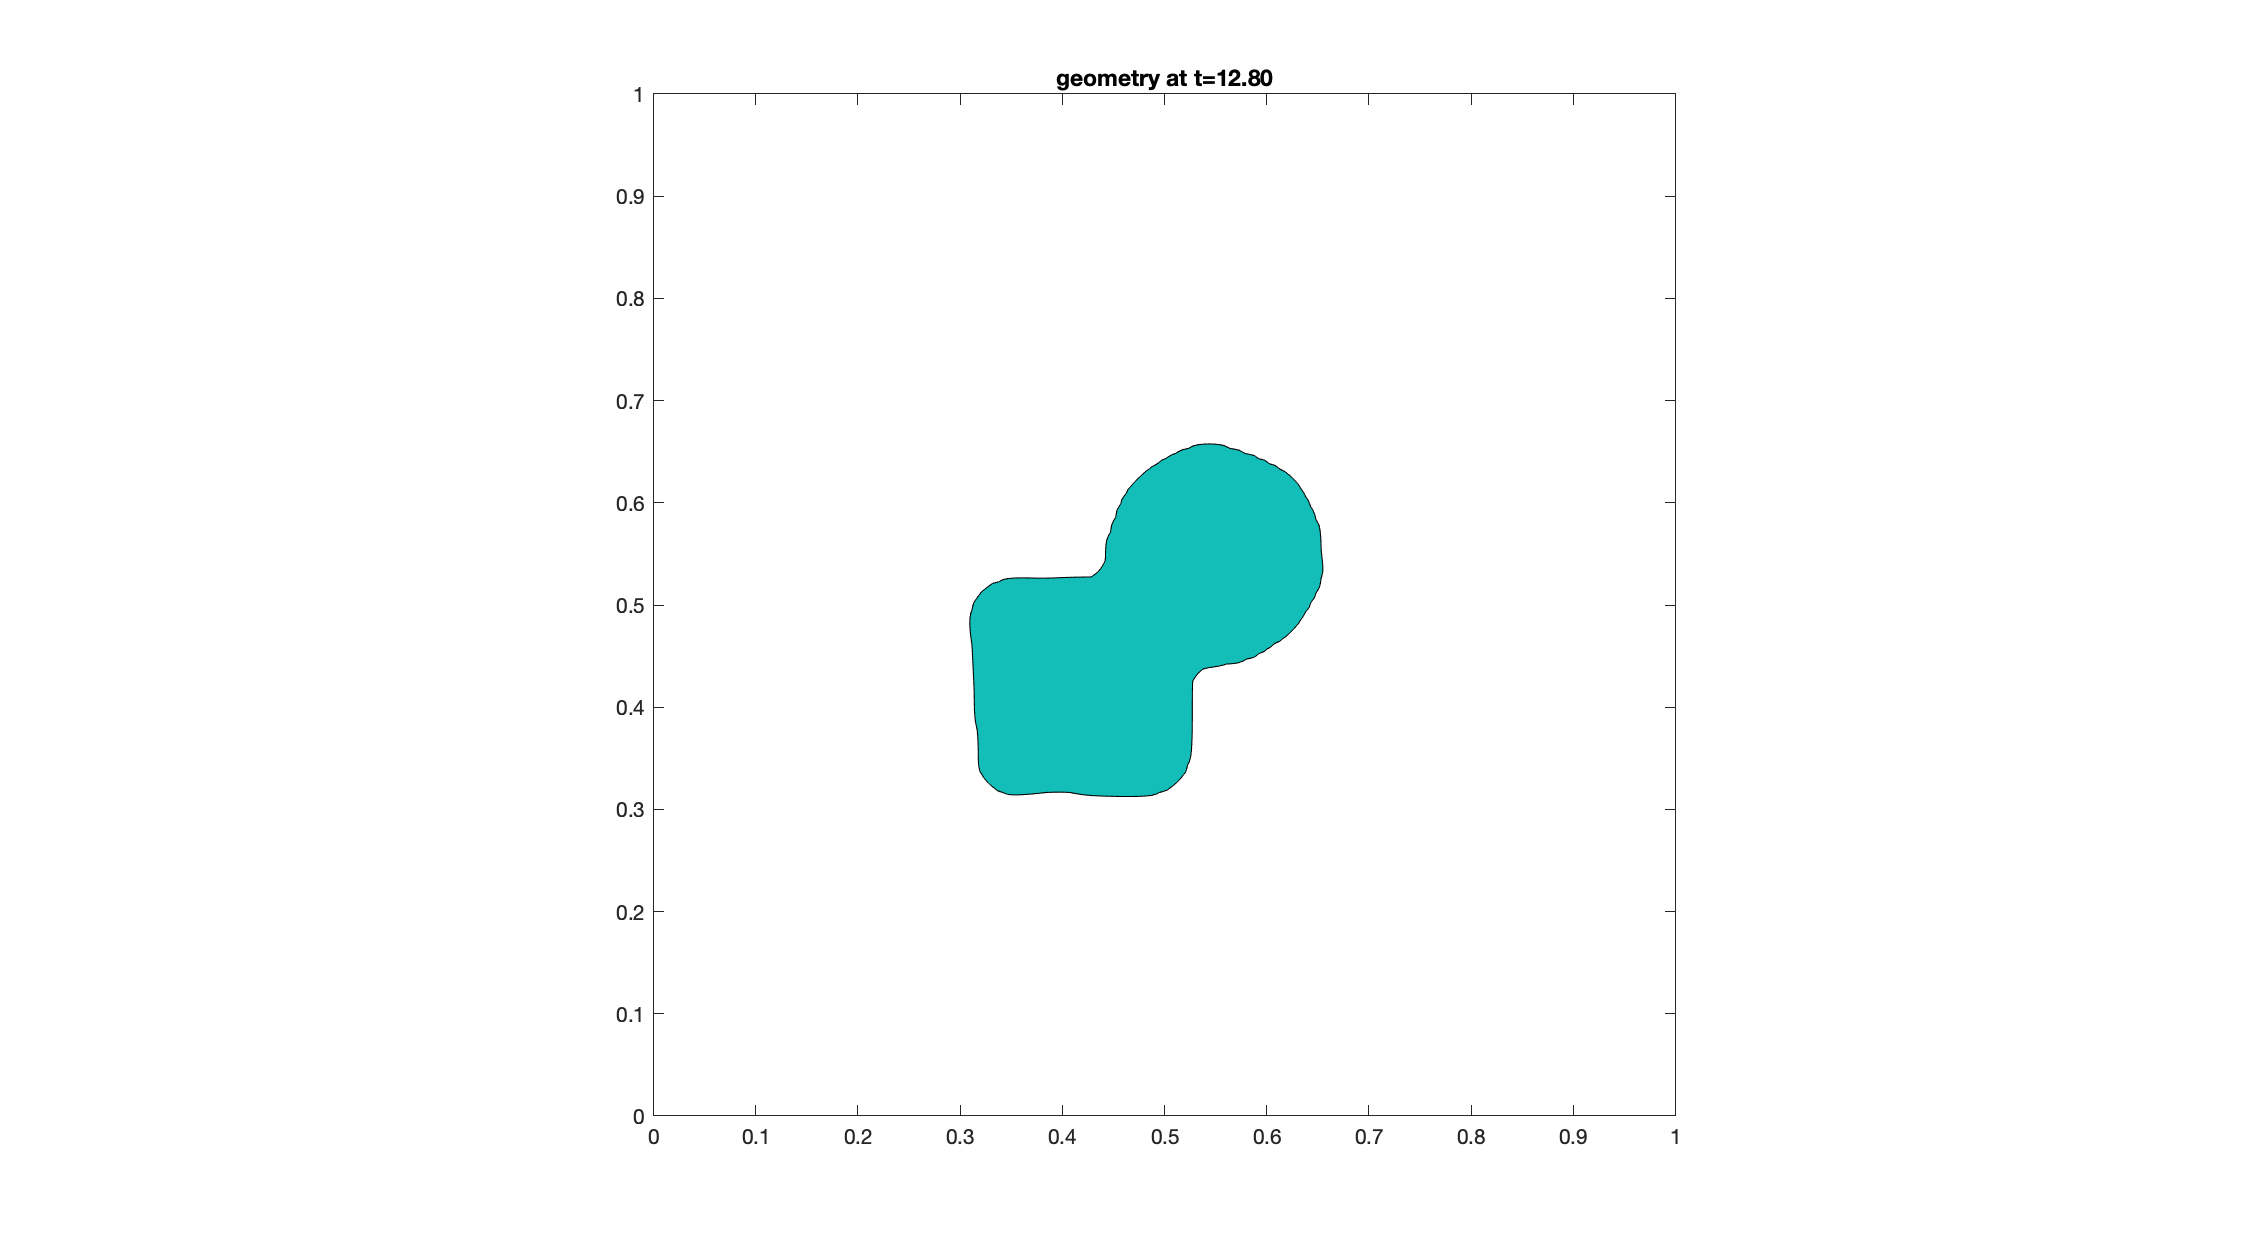
\includegraphics[width=0.5\textwidth]{ex6final.png}}
  \caption{$\sigma = 13\times 10^{-5}$, $p = 9.9$, $\gamma=5.5\times 10^{-15.25}$}
\end{figure}
This caused the contour to stop ``sooner'' and therefore the image is wider in some places compared to the original image. I then ran a test on a spine-dendrite image:
\clearpage
\begin{figure}[h!]
    \centering
    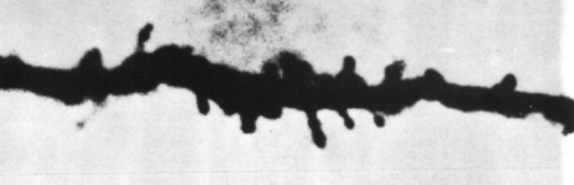
\includegraphics[width=\linewidth]{imagedend.png}
\end{figure}

I modified the level set function so that the contour would begin outside the image.
\begin{figure}[h!]
  \centering
  \subfloat[]{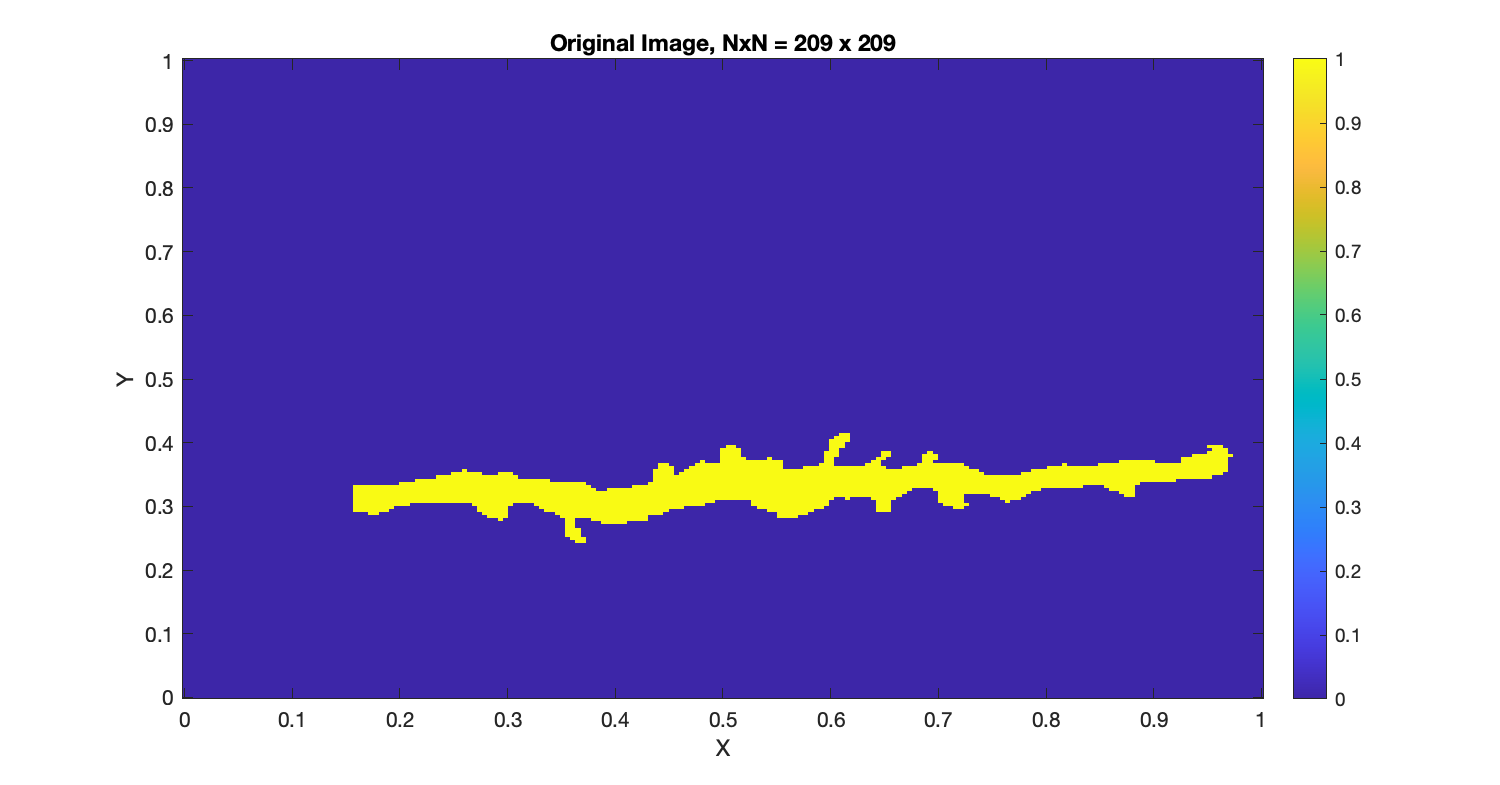
\includegraphics[width=0.5\textwidth]{ex7original.png}}
  \hfill
  \subfloat[]{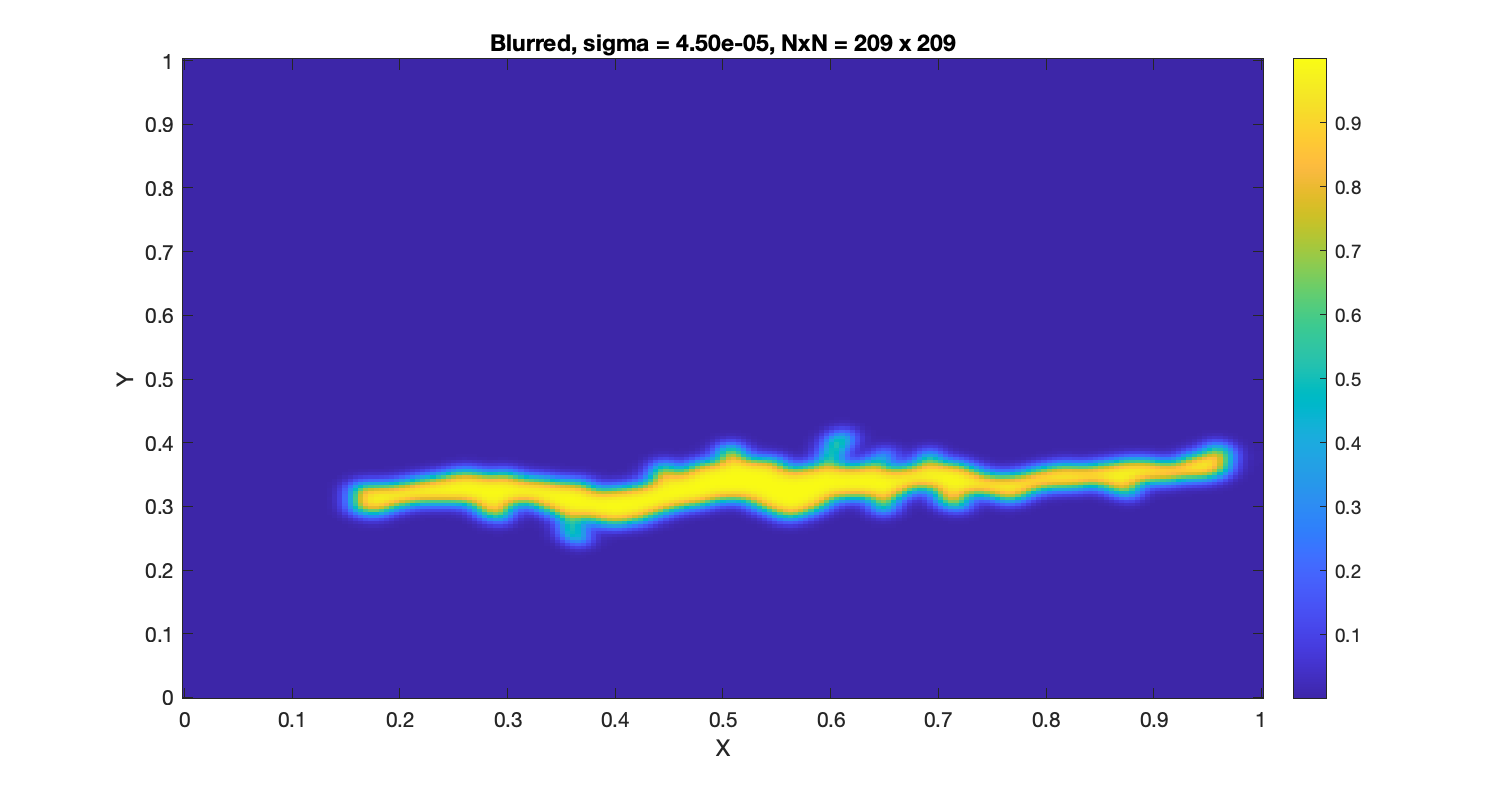
\includegraphics[width=0.5\textwidth]{ex7blurred.png}}\\
  \subfloat[]{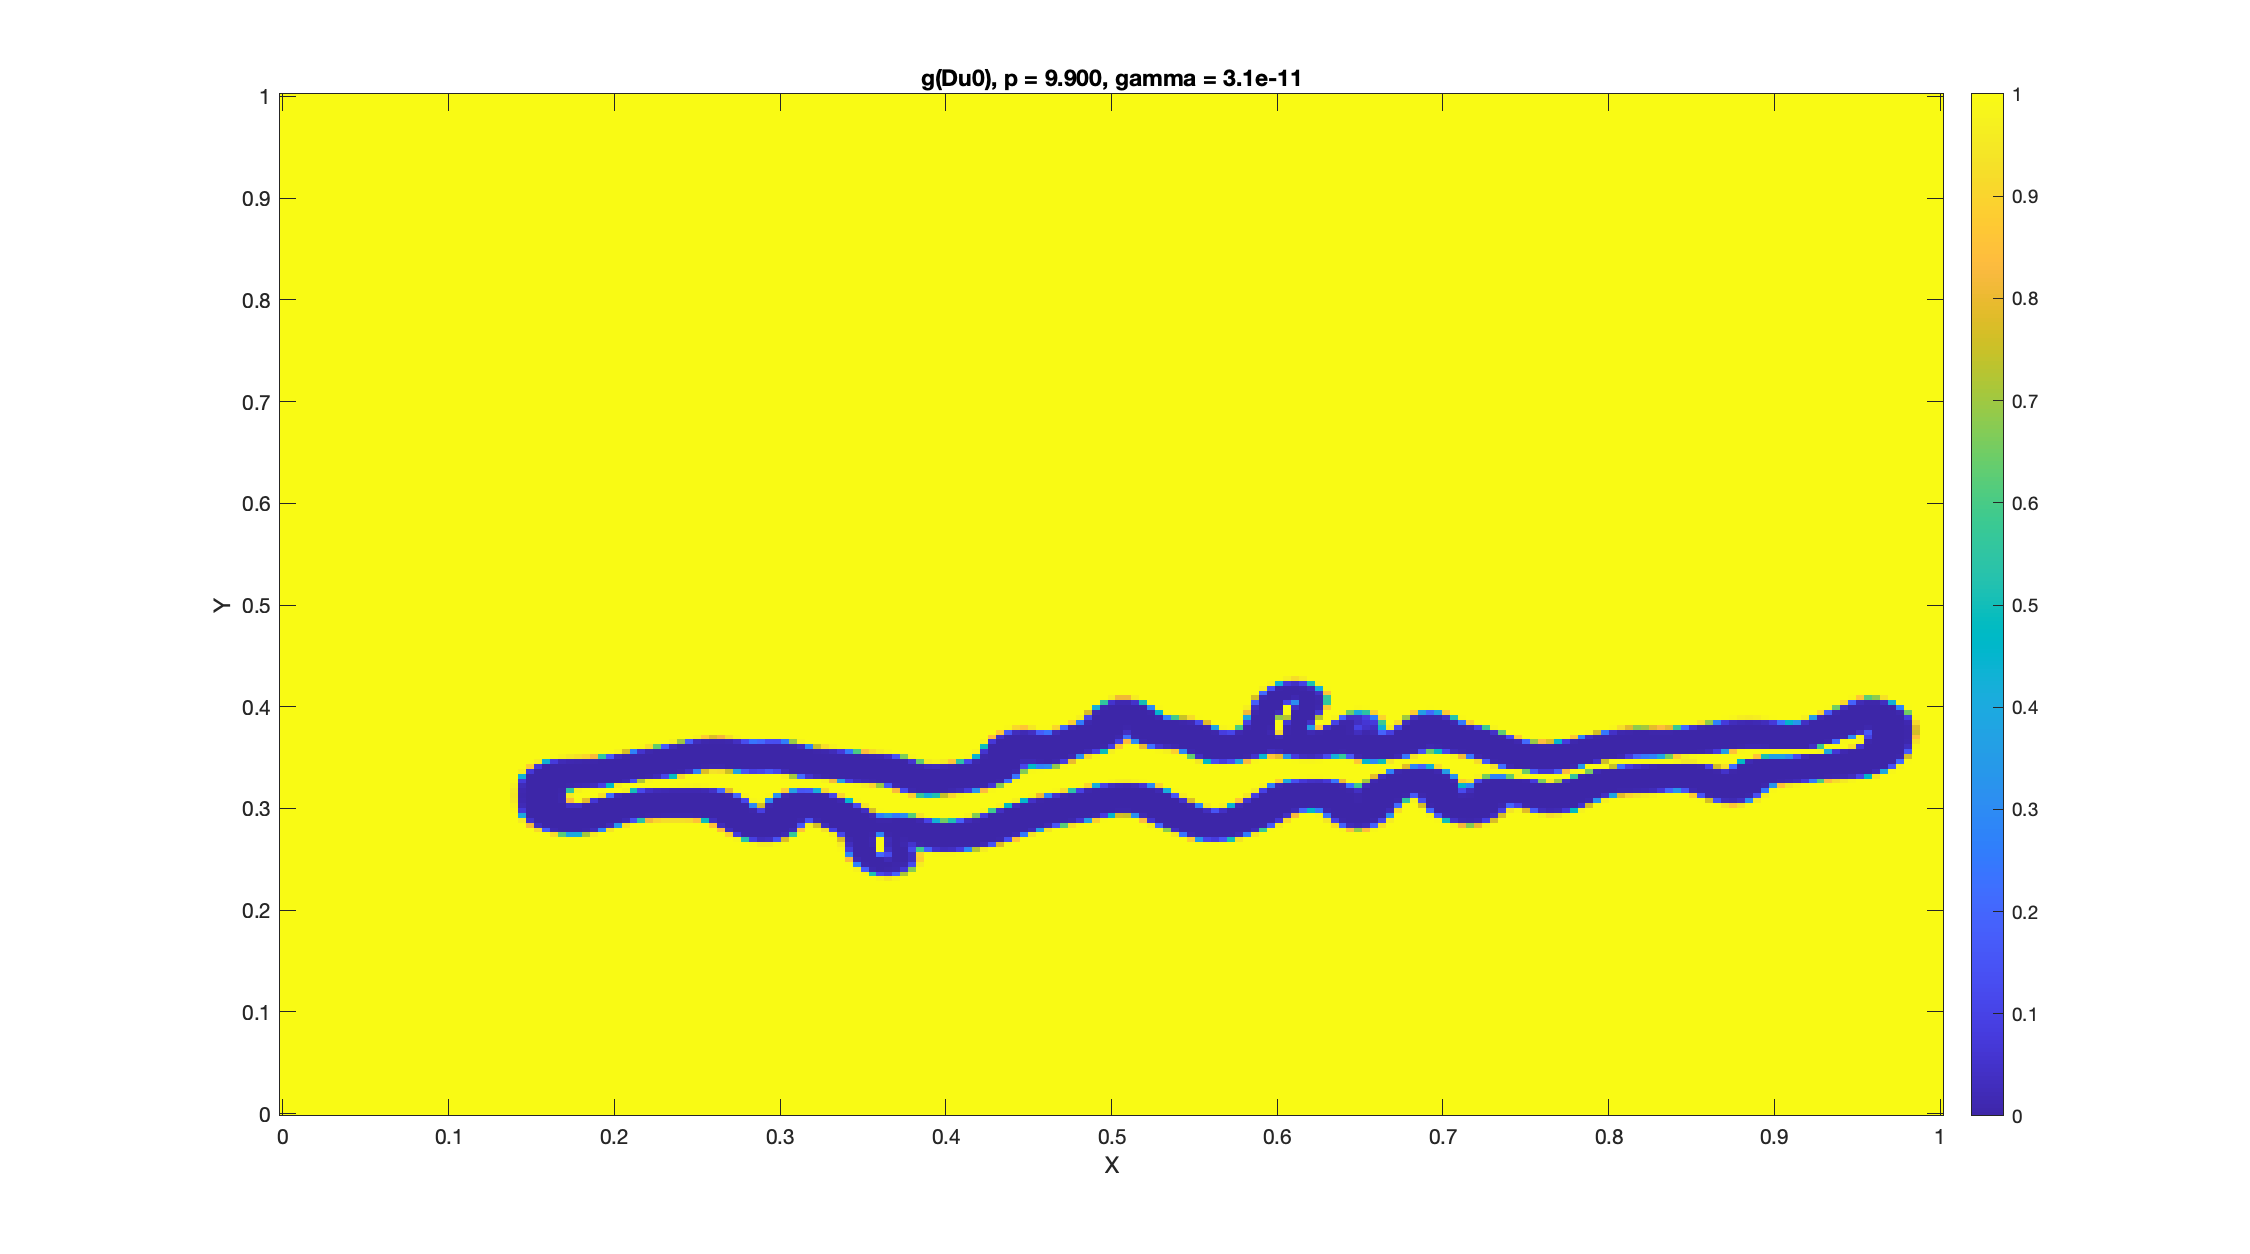
\includegraphics[width=0.5\textwidth]{ex7speedfunction_with_u0.png}}
  \\
  \subfloat[]{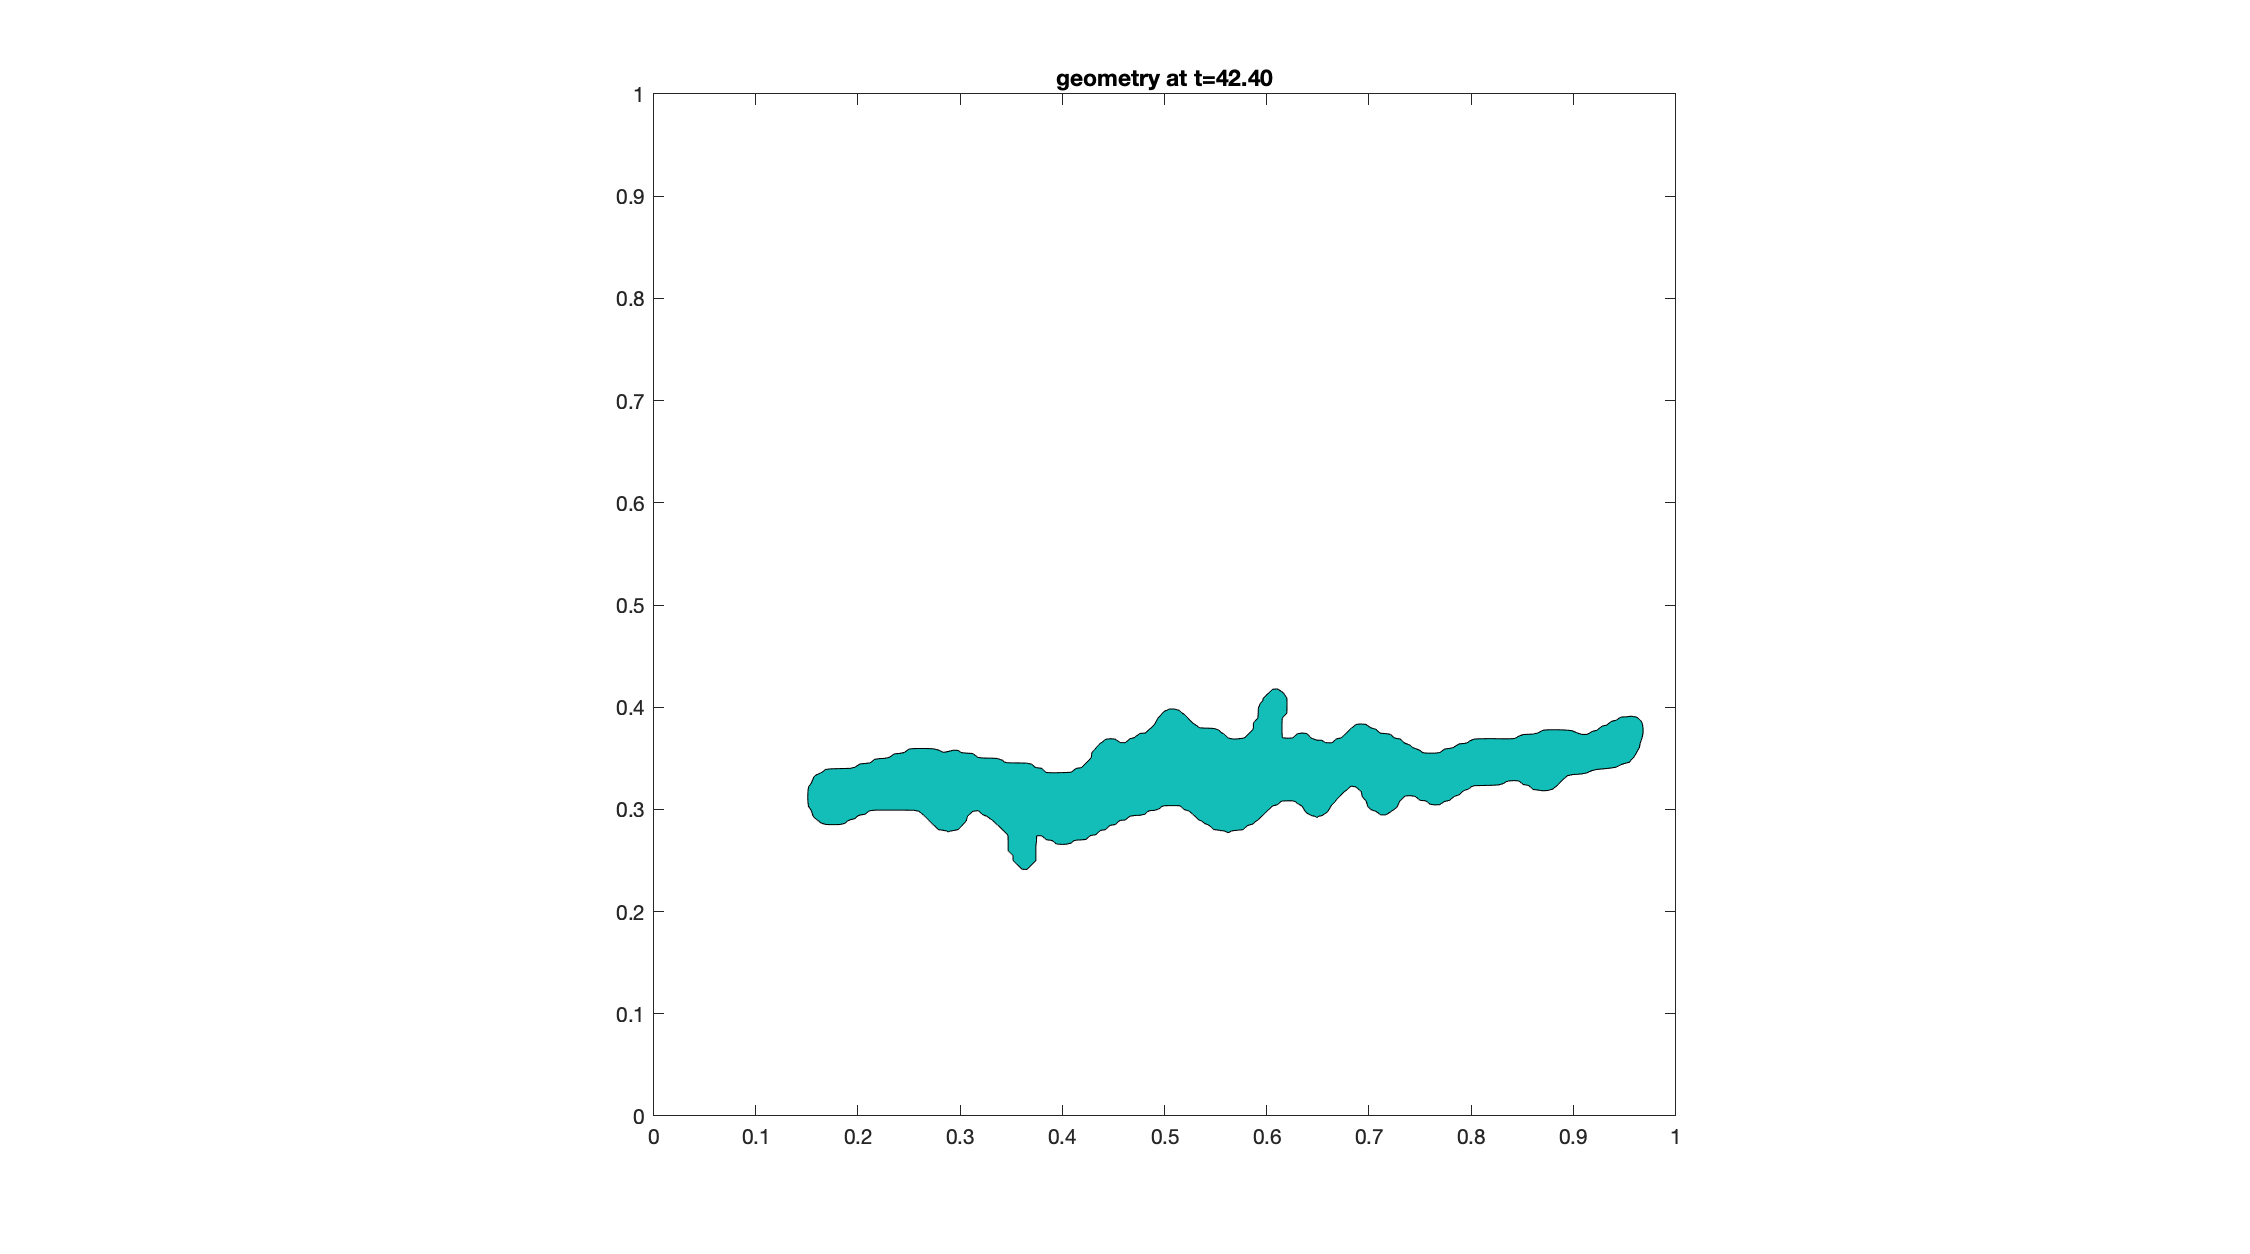
\includegraphics[width=0.5\textwidth]{ex7final.png}}
  \caption{$\sigma = 13\times 10^{-5}$, $p = 9.9$, $\gamma=5.5\times 10^{-11.25}$}
\end{figure}

I was able to use the same parameters as before and still capture the spines that are protruding from the dendrite.
\section{Conclusion}
In this section I will discuss the challenges faced in the project and the parts of the project that need refinement and/or completion. One of the challenges faced in this project is properly defining the edge detector for the moving image front, in particular making it robust against noise. For instance, what parameters of $p$ and $\gamma$ and the amount of smoothing are necessary to ensure that the front continues to ``move'' towards the image and not get stuck on a noisy section. If enough Gaussian smoothing is applied then the noisy part smooths away; however, this is at the cost of destroying feature and landmarks on the image we wish to detect. The choice of parameters  $\gamma$ and $p$ depend on the smoothing amount and also on the image resolution, if the image is too poor and too much smoothing then the moving front has no chance of constructing the image features. These scenarios involve trial error to determine the ``best'' parameters so that the image is reasonably reconstructed. Some items that need to be address are
\begin{itemize}
    \item Implement the Mumford-Shah functional \cite{doi:10.1002/cpa.3160430805}
\[
{\displaystyle E[J,B]=C\int _{D}(I({\vec {x}})-J({\vec {x}}))^{2}\,\mathrm {d} {\vec {x}}+A\int _{D/B}{\vec {\nabla }}J({\vec {x}})\cdot {\vec {\nabla }}J({\vec {x}})\,\mathrm {d} {\vec {x}}+B\int _{B}\ ds}
\]
optimizing this functional leads to a criteria for segmenting an image into sub-image regions and Ambrosio-Tortorelli give an algorithm for achieving the minimum and also show the minimum is well-defined.
\item Implement the gradient vector flow methodology
    \item Test the two implementations above on 2d neuron geometries e.g. and 2d graph essentially
    \item Then implement on 3d geometries of neurons
\end{itemize}
\bibliographystyle{siamplain}
\nocite{*} 
\bibliography{references}
\end{document}
